\documentclass[11pt,a4paper]{article}

% --- Page Geometry ---
\usepackage[a4paper, margin=2.2cm, headheight=14pt]{geometry}

% --- Mathematics & Physics Packages ---
\usepackage{amsmath, amssymb, amsfonts, bm, mathtools}

% --- Professional Tables ---
\usepackage{booktabs, longtable, array}

% --- Lists & Typography ---
\usepackage{enumitem}
\usepackage{xcolor}

% --- Source Code Listings ---
\usepackage{listings}

% --- Advanced Boxed Environments for Student Learning ---
\usepackage{tcolorbox}
\tcbuselibrary{skins, breakable}

% --- Native Vector Graphics ---
\usepackage{pgfplots}
\pgfplotsset{compat=1.18}
\usetikzlibrary{patterns, arrows.meta, positioning, calc}

% --- Running Headers & Footers (Strictly Student Copy) ---
\usepackage{fancyhdr}
\pagestyle{fancy}
\fancyhf{}
\fancyhead[L]{\small\color{blue!60!black}\textbf{PH7302: Condensed Matter Physics}}
\fancyhead[R]{\small\color{gray!80!black}Module 3: Free Electron Theory (Student Copy)}
\fancyfoot[C]{\small\thepage}
\renewcommand{\headrulewidth}{0.5pt}
\renewcommand{\footrulewidth}{0.4pt}

% --- Section Titles Styling ---
\usepackage{titlesec}
\titleformat{\section}{\large\bfseries\color{blue!60!black}}{\thesection}{1em}{}[\titlerule]
\titleformat{\subsection}{\normalsize\bfseries\color{blue!45!black}}{\thesubsection}{1em}{}
\titleformat{\subsubsection}{\small\bfseries\color{black}}{\thesubsubsection}{1em}{}

% --- Hyperlinks Configuration ---
\usepackage{hyperref}
\hypersetup{
    colorlinks=true,
    linkcolor=blue!60!black,
    citecolor=blue!60!black,
    urlcolor=blue!60!black,
    pdfauthor={Department of Physics, NIT Calicut},
    pdftitle={Module 3: Free Electron Theory --- Student Copy},
    pdfsubject={PH7302 Condensed Matter Physics}
}

% --- Color Palette ---
\definecolor{codebg}{rgb}{0.96, 0.96, 0.96}
\definecolor{codeframe}{rgb}{0.75, 0.75, 0.75}
\definecolor{boxblue}{rgb}{0.12, 0.28, 0.54}
\definecolor{boxteal}{rgb}{0.08, 0.45, 0.40}
\definecolor{boxpurple}{rgb}{0.40, 0.15, 0.55}
\definecolor{boxorange}{rgb}{0.75, 0.35, 0.05}

% --- Listings Settings for Python Scripts ---
\lstset{
    language=Python,
    backgroundcolor=\color{codebg},
    frame=single,
    rulecolor=\color{codeframe},
    basicstyle=\ttfamily\small,
    breaklines=true,
    keywordstyle=\color{blue!80!black}\bfseries,
    commentstyle=\color{green!50!black}\itshape,
    stringstyle=\color{red!70!black},
    numbers=left,
    numberstyle=\tiny\color{gray},
    numbersep=6pt,
    tabsize=4,
    showstringspaces=false
}

% --- Custom Mathematical Macros ---
\newcommand{\ket}[1]{\left|#1\right\rangle}
\newcommand{\bra}[1]{\left\langle #1\right|}
\newcommand{\braket}[2]{\left\langle #1 \middle| #2 \right\rangle}
\newcommand{\expect}[1]{\left\langle #1 \right\rangle}
\newcommand{\vb}[1]{\mathbf{#1}}

% --- Student Learning Environments (Replacing Instructor Boxes) ---
% 1. Conceptual Checkpoint
\newtcolorbox{checkpointbox}[1]{%
    colback=blue!3!white,
    colframe=boxblue,
    fonttitle=\bfseries\small,
    title={Conceptual Checkpoint: #1},
    arc=2mm,
    boxrule=0.9pt,
    breakable,
    enhanced,
    before upper={\parindent0pt}
}

% 2. Study Takeaway
\newtcolorbox{takeawaybox}[1]{%
    colback=teal!3!white,
    colframe=boxteal,
    fonttitle=\bfseries\small,
    title={Study Takeaway: #1},
    arc=2mm,
    boxrule=0.9pt,
    breakable,
    enhanced,
    before upper={\parindent0pt}
}

% 3. Problem-Solving Strategy
\newtcolorbox{methodbox}[1]{%
    colback=purple!3!white,
    colframe=boxpurple,
    fonttitle=\bfseries\small,
    title={Problem-Solving Strategy: #1},
    arc=2mm,
    boxrule=0.9pt,
    breakable,
    enhanced,
    before upper={\parindent0pt}
}

% 4. Common Misconception & Pitfall
\newtcolorbox{pitfallbox}[1]{%
    colback=orange!4!white,
    colframe=boxorange,
    fonttitle=\bfseries\small,
    title={Common Misconception \& Pitfall: #1},
    arc=2mm,
    boxrule=0.9pt,
    breakable,
    enhanced,
    before upper={\parindent0pt}
}

% 5. In-Text Worked Example
\newtcolorbox{examplebox}[2]{%
    colback=gray!3!white,
    colframe=blue!85!black,
    fonttitle=\bfseries\small,
    title={Worked Example: #1},
    label={#2},
    arc=2mm,
    boxrule=1.0pt,
    breakable,
    enhanced,
    before upper={\parindent0pt}
}

% 6. Upfront Assignment Part Box
\newtcolorbox{assignmentbox}[1]{%
    colback=blue!2!white,
    colframe=blue!60!black,
    fonttitle=\bfseries\normalsize,
    title={#1},
    arc=2mm,
    boxrule=1.0pt,
    breakable,
    enhanced,
    before upper={\parindent0pt}
}


\begin{document}

% --- Title Block ---
\title{%
    \vspace{-1.5cm}
    \textbf{\LARGE Module 3: Free Electron Theory}\\[0.35cm]
    \Large Student Copy --- Comprehensive Lecture \& Tutorial Guide\\[0.25cm]
    \large\color{blue!60!black}\textbf{PH7302: Condensed Matter Physics / Electronic Structure of Materials}
}
\author{%
    \textbf{Department of Physics}\\
    \text{National Institute of Technology Calicut}
}
\date{Academic Year 2026--2027}
\maketitle

\vspace{-0.5cm}
\begin{abstract}
\noindent This document constitutes the unified, self-contained student edition for \textbf{Module 3: Free Electron Theory and the Origin of Energy Bands} in PH7302 Condensed Matter Physics. It synthesizes classical Drude transport theory, quantum Sommerfeld Fermi gas statistics, density of states across dimensions, the quantum Boltzmann Transport Equation (BTE), electronic and thermal conductivity, the Wiedemann--Franz law, thermoelectric phenomena (Seebeck, Peltier, Thomson, and Mott formula), failure modes of the free electron approximation, Bloch's theorem, nearly free electron band gap formation, and Fermi surface experimental probes (de Haas--van Alphen quantum oscillations). The guide features an upfront assignment problem set of 26 curated problems, 18 step-by-step solved in-text numerical and conceptual examples, targeted student learning boxes, and interactive Python simulation scripts.
\end{abstract}

\vspace{0.3cm}

% --- Student Study Guide ---
\section*{How to Use This Student Edition}
\addcontentsline{toc}{section}{How to Use This Student Edition}

This student edition has been structured to guide you from foundational physical concepts to advanced mathematical mastery of electronic transport and band formation. To maximize your learning efficiency, consider the following study roadmap:

\begin{enumerate}[leftmargin=*]
    \item \textbf{Work the Upfront Assignment Continuously}: The section immediately following the Table of Contents contains the complete module assignment problem set (26 problems across 5 parts). Each problem provides exact parameters and concise final numerical answers or hints in brackets (\texttt{[Ans: ...]}). Attempt each problem as soon as you finish the corresponding lecture chapter. Intermediate derivations are intentionally omitted to encourage active problem-solving.
    \item \textbf{Study the In-Text Worked Examples}: Embedded within Chapters 1--10 are 18 fully solved worked examples. Each example breaks down the physical setup, algebraic substitutions in SI units, unit conversions, and physical interpretation. Work through these derivations with pen and paper before attempting the assignment exercises.
    \item \textbf{Engage with the Conceptual Learning Boxes}:
    \begin{itemize}[leftmargin=1.5cm]
        \item \textbf{Conceptual Checkpoints}: Probe deeper into physical principles (e.g., screening, quasiparticles, and wave interference).
        \item \textbf{Study Takeaways}: Highlight overarching physical takeaways to commit to memory.
        \item \textbf{Problem-Solving Strategies}: Provide systematic calculation recipes for exams and research.
        \item \textbf{Common Misconceptions \& Pitfalls}: Flag algebraic traps, unit inconsistencies, and physical fallacies.
    \end{itemize}
    \item \textbf{Run the Computational Demonstrations}: Appendix~A includes 5 complete Python scripts illustrating key quantum phenomena: Fermi energy calculation, thermal smearing of the Fermi edge, low-temperature specific heat fitting, zone-boundary band gap splitting, and de Haas--van Alphen oscillations. Executing and modifying these scripts will build concrete numerical intuition.
\end{enumerate}

\vspace{0.3cm}

% --- Module Overview & Syllabus Alignment ---
\section{Module Overview and Syllabus Alignment}
\label{sec:overview}

The content of Module 3 spans classical to quantum models of conduction electrons, culminating in the necessity of energy band theory:

\begin{table}[ht]
\centering
\small
\renewcommand{\arraystretch}{1.25}
\begin{tabular}{p{2.2cm} p{5.0cm} p{8.2cm}}
\toprule
\textbf{Chapter} & \textbf{Core Topic} & \textbf{Syllabus Learning Outcomes \& Competencies} \\
\midrule
\textbf{Chapter 1} & Classical Drude Theory & Equations of motion, drift velocity, DC/AC conductivity, mobility, velocity hierarchy, mean free path paradox, Drude Lorenz number, Hall effect. \\
\textbf{Chapter 2} & Sommerfeld Free Electron Gas & 1D/3D wells, periodic boundary conditions, $k$-space quantization, Fermi sphere, $k_F, p_F, E_F, v_F, T_F$, empirical electron density formula and metal data. \\
\textbf{Chapter 3} & Density of States \& Ground State & Phase-space cell quantization, PBC method, 1D/2D/3D comparison, ground state energy $U_0 = \frac{3}{5}NE_F$, Fermi pressure $P_0$, electronic bulk modulus $B$. \\
\textbf{Chapter 4} & Quantum Statistics \& Specific Heat & Fermi--Dirac distribution, chemical potential $\mu(T)$, Sommerfeld integral expansion, linear $C_{el} = \gamma T$, Debye crossover $C/T = \gamma + \beta T^2$, Pauli paramagnetism. \\
\textbf{Chapter 5} & Electrical \& Thermal Transport & Boltzmann Transport Equation in RTA, linearized distribution, Fermi surface integration, recovery of $\sigma$, Matthiessen's rule, quantum thermal conductivity, Wiedemann--Franz law ($L = \frac{\pi^2}{3}(k_B/e)^2$). \\
\textbf{Chapter 6} & Thermoelectric Phenomena & Seebeck effect, Peltier effect, Thomson effect, Kelvin relations, microscopic Peltier flux derivation, Mott formula for thermopower $S \approx -\frac{\pi^2 k_B}{2e}(T/T_F)$. \\
\textbf{Chapter 7} & Model Limitations \& Band Origin & Positive Hall coefficients, divalent metals, magnetoresistance, distinction between conductors/insulators, periodic potential necessity, coupled-oscillator band formation. \\
\textbf{Chapter 8} & Periodic Potential \& Bloch Theorem & Translation operators, Bloch's theorem proof, crystal momentum $\hbar\vb{k}$, Born--von Karman boundary, extended, reduced, and periodic zone schemes. \\
\textbf{Chapter 9} & Nearly Free Electron Model & Weak potential perturbation, zone-boundary degeneracy, 2-state secular equation, band gap $\Delta E = 2|V_{\vb{G}}|$, standing waves $\psi_\pm$ and electrostatic energy splitting. \\
\textbf{Chapter 10} & Fermi Surfaces \& Probes & Fermi surface construction, Landau levels, cyclotron resonance, semiclassical Onsager relation, de Haas--van Alphen oscillations, extremal cross-sections. \\
\textbf{Chapter 11} & Capstone Problem Solving & Comprehensive multi-concept tutorial problems integrating thermodynamics, transport, band gaps, and quantum oscillations. \\
\bottomrule
\end{tabular}
\caption{Structure, syllabus coverage, and learning outcomes for Module 3.}
\label{tab:syllabus_map}
\end{table}

\clearpage

% --- Table of Contents ---
\tableofcontents
\clearpage

% --- Physical Constants Reference Table ---
\section{Physical Constants and Useful Identities}
\label{sec:constants}

The following standard physical constants and unit conversions are used consistently throughout this module:

\begin{table}[ht]
\centering
\small
\renewcommand{\arraystretch}{1.2}
\begin{tabular}{llll}
\toprule
\textbf{Quantity} & \textbf{Symbol} & \textbf{SI Value} & \textbf{Alternate / Practical Value} \\
\midrule
Planck constant & $h$ & $6.6261 \times 10^{-34}\ \mathrm{J\cdot s}$ & $4.1357 \times 10^{-15}\ \mathrm{eV\cdot s}$ \\
Reduced Planck constant & $\hbar = h/(2\pi)$ & $1.0546 \times 10^{-34}\ \mathrm{J\cdot s}$ & $6.5821 \times 10^{-16}\ \mathrm{eV\cdot s}$ \\
Electron rest mass & $m_e$ & $9.1094 \times 10^{-31}\ \mathrm{kg}$ & $0.5110\ \mathrm{MeV}/c^2$ \\
Elementary charge & $e$ & $1.6022 \times 10^{-19}\ \mathrm{C}$ & --- \\
Boltzmann constant & $k_B$ & $1.3807 \times 10^{-23}\ \mathrm{J/K}$ & $8.6173 \times 10^{-5}\ \mathrm{eV/K}$ \\
Avogadro constant & $N_A$ & $6.0221 \times 10^{23}\ \mathrm{mol^{-1}}$ & --- \\
Bohr magneton & $\mu_B = e\hbar/(2m_e)$ & $9.2740 \times 10^{-24}\ \mathrm{J/T}$ & $5.7884 \times 10^{-5}\ \mathrm{eV/T}$ \\
Permeability of vacuum & $\mu_0$ & $4\pi \times 10^{-7}\ \mathrm{H/m}$ & $1.2566 \times 10^{-6}\ \mathrm{N/A^2}$ \\
Permittivity of vacuum & $\epsilon_0$ & $8.8542 \times 10^{-12}\ \mathrm{F/m}$ & --- \\
Universal gas constant & $R = N_A k_B$ & $8.3145\ \mathrm{J/(mol\cdot K)}$ & --- \\
Sommerfeld Lorenz number & $L = \frac{\pi^2}{3}(k_B/e)^2$ & $2.4428 \times 10^{-8}\ \mathrm{W\,\Omega\,K^{-2}}$ & --- \\
\bottomrule
\end{tabular}
\caption{Fundamental physical constants adopted in this text.}
\label{tab:constants}
\end{table}

\subsection*{Useful Numerical Conversions and Benchmarks}
\begin{itemize}[leftmargin=1.5cm]
    \item $1\ \mathrm{eV} = 1.6022 \times 10^{-19}\ \mathrm{J}$.
    \item Thermal energy scale at $T = 300\ \mathrm{K}$: $k_B T = 0.02585\ \mathrm{eV} \approx \frac{1}{40}\ \mathrm{eV}$.
    \item Free electron coefficient: $\frac{\hbar^2}{2m_e} \approx 3.81\ \mathrm{eV\cdot\text{\AA}^2} = 6.10 \times 10^{-39}\ \mathrm{J\cdot m^2}$.
    \item Wavevector to energy conversion: $E(\mathrm{eV}) \approx 3.81 \times [k(\text{\AA}^{-1})]^2$.
    \item $1\ \mathrm{atm} = 1.01325 \times 10^5\ \mathrm{Pa} = 1.01325 \times 10^5\ \mathrm{N/m^2}$.
\end{itemize}

\clearpage


% =========================================================================
% UPFRONT ASSIGNMENT: MODULE 3
% =========================================================================
\section*{Assignment: Module 3 --- Free Electron Theory and Band Origin}
\addcontentsline{toc}{section}{Assignment: Module 3 --- Practice Problems Set}
\label{sec:assignment_module3}

\noindent\fbox{%
\parbox{\dimexpr\textwidth-2\fboxsep-2\fboxrule\relax}{%
\small
\textbf{Instructions for Students:} This assignment covers the theoretical derivations, physical concepts, and quantitative problem-solving techniques developed across Module 3. Problems are organized into five thematic parts corresponding to lecture chapters. Final answers and essential hints are provided in brackets (\texttt{[Ans: ...]}) to facilitate self-evaluation. Full step-by-step model derivations for representative problem archetypes are provided as in-text worked examples within the respective lecture chapters.
}%
}

\vspace{0.4cm}

% -------------------------------------------------------------------------
\subsection*{Part I: Classical Drude Theory \& Electrical Transport}
% -------------------------------------------------------------------------

\begin{enumerate}[label=\textbf{\arabic*.}, leftmargin=*]
    \item \textbf{Aluminum Relaxation Time and Drift Kinetics}:\\
    Metallic aluminum has an electrical conductivity $\sigma = 3.5 \times 10^7\ \Omega^{-1}\mathrm{m}^{-1}$ at room temperature ($300\ \mathrm{K}$) and a conduction electron concentration $n = 1.8 \times 10^{29}\ \mathrm{m}^{-3}$.
    \begin{enumerate}[label=(\alph*)]
        \item Calculate the momentum relaxation time $\tau$ using the Drude model.
        \item If an electric field of $E = 0.50\ \mathrm{V/m}$ is applied across an aluminum wire, determine the steady-state electron drift velocity $v_d$.
        \item Compute the net distance traversed by an electron in $1.0\ \mathrm{second}$ of steady drift.
    \end{enumerate}
    \textbf{[Ans:} (a) $\tau \approx 6.9 \times 10^{-15}\ \mathrm{s} = 6.9\ \mathrm{fs}$; (b) $v_d \approx 6.07 \times 10^{-4}\ \mathrm{m/s} = 0.61\ \mathrm{mm/s}$; (c) $d \approx 0.61\ \mathrm{mm}$\textbf{]}

    \item \textbf{Residual Resistivity Ratio (RRR) of Copper}:\\
    A high-purity copper specimen exhibits an electrical resistivity of $\rho(300\ \mathrm{K}) = 1.70 \times 10^{-8}\ \Omega\cdot\mathrm{m}$ at room temperature, while at liquid helium temperature ($4.2\ \mathrm{K}$) its resistivity falls to $\rho(4.2\ \mathrm{K}) = 1.00 \times 10^{-10}\ \Omega\cdot\mathrm{m}$.
    \begin{enumerate}[label=(\alph*)]
        \item Calculate the ratio of momentum relaxation times $\tau(4.2\ \mathrm{K}) / \tau(300\ \mathrm{K})$.
        \item Identify the dominant microscopic scattering mechanism at $300\ \mathrm{K}$ and at $4.2\ \mathrm{K}$, and calculate the percentage of room-temperature resistance attributable to thermal phonons.
    \end{enumerate}
    \textbf{[Ans:} (a) $\tau(4.2\ \mathrm{K})/\tau(300\ \mathrm{K}) = 170$; (b) Phonon scattering accounts for $99.4\%$ of room-temperature resistivity; at $4.2\ \mathrm{K}$, static impurity and defect scattering dominates exclusively\textbf{]}

    \item \textbf{Comprehensive Transport Analysis of Metallic Copper}:\\
    Consider monovalent metallic copper with mass density $\rho_m = 8.96\ \mathrm{g/cm^3}$, atomic mass $A = 63.55\ \mathrm{g/mol}$, and measured electrical resistivity $\rho = 1.70 \times 10^{-8}\ \Omega\cdot\mathrm{m}$ at $300\ \mathrm{K}$. Under an applied field $E = 1.0\ \mathrm{V/m}$:
    \begin{enumerate}[label=(\alph*)]
        \item Determine the conduction electron density $n$.
        \item Evaluate the Fermi wavevector $k_F$, Fermi energy $E_F$, and Fermi velocity $v_F$.
        \item Calculate the momentum relaxation time $\tau$ and the quantum mean free path $l = v_F \tau$.
        \item Calculate the average drift velocity $v_d$.
        \item Determine the dimensionless ratio $v_d / v_F$.
    \end{enumerate}
    \textbf{[Ans:} (a) $n \approx 8.49 \times 10^{28}\ \mathrm{m^{-3}}$; (b) $k_F \approx 1.36 \times 10^{10}\ \mathrm{m^{-1}}$, $E_F \approx 7.04\ \mathrm{eV}$, $v_F \approx 1.57 \times 10^6\ \mathrm{m/s}$; (c) $\tau \approx 2.46 \times 10^{-14}\ \mathrm{s}$, $l \approx 387\ \text{\AA}$; (d) $v_d \approx 4.32 \times 10^{-3}\ \mathrm{m/s} = 4.32\ \mathrm{mm/s}$; (e) $v_d/v_F \approx 2.75 \times 10^{-9}$\textbf{]}

    \item \textbf{Matthiessen's Rule and Low-Temperature Mean Free Path}:\\
    Applying Matthiessen's rule $\rho(T) = \rho_0 + \rho_{\mathrm{ph}}(T)$ to the copper sample from Assignment~2:
    \begin{enumerate}[label=(\alph*)]
        \item Determine the residual resistivity $\rho_0$ and the phonon-induced resistivity $\rho_{\mathrm{ph}}(300\ \mathrm{K})$.
        \item Given that the room-temperature mean free path is $l(300\ \mathrm{K}) \approx 400\ \text{\AA}$, calculate the electron mean free path at liquid helium temperature $l(4.2\ \mathrm{K})$.
    \end{enumerate}
    \textbf{[Ans:} (a) $\rho_0 = 1.00 \times 10^{-10}\ \Omega\cdot\mathrm{m}$, $\rho_{\mathrm{ph}}(300\ \mathrm{K}) = 1.69 \times 10^{-8}\ \Omega\cdot\mathrm{m}$; (b) $l(4.2\ \mathrm{K}) = 170 \times 400\ \text{\AA} = 68{,}000\ \text{\AA} = 6.8\ \mu\mathrm{m}$\textbf{]}

    \item \textbf{Defect Scattering in Cold-Worked and Annealed Copper}:\\
    A heavily cold-worked copper wire has an electrical resistivity of $\rho = 2.00 \times 10^{-8}\ \Omega\cdot\mathrm{m}$ at $300\ \mathrm{K}$. After thorough high-temperature annealing (which removes dislocations and internal grain boundaries), its resistivity decreases to $1.70 \times 10^{-8}\ \Omega\cdot\mathrm{m}$. What percentage of the initial room-temperature resistivity was caused by work-induced lattice defects?
    \textbf{[Ans:} Defect percentage $= (\Delta\rho/\rho_{\mathrm{initial}}) \times 100\% = (0.30/2.00) \times 100\% = 15.0\%$\textbf{]}
\end{enumerate}

\vspace{0.4cm}

% -------------------------------------------------------------------------
\subsection*{Part II: Quantum Free Electron Gas \& Fermi--Dirac Statistics}
% -------------------------------------------------------------------------

\begin{enumerate}[label=\textbf{\arabic*.}, resume, leftmargin=*]
    \item \textbf{Fermi Energy and Characteristic Temperatures of Sodium}:\\
    Metallic sodium crystallizes in a BCC structure with one valence electron per atom, yielding an electron density $n = 2.65 \times 10^{28}\ \mathrm{m}^{-3}$.
    \begin{enumerate}[label=(\alph*)]
        \item Calculate the Fermi wavevector $k_F$ and Fermi momentum $p_F$.
        \item Calculate the Fermi energy $E_F$ in Joules and in electron-volts.
        \item Determine the Fermi temperature $T_F$ and Fermi velocity $v_F$.
    \end{enumerate}
    \textbf{[Ans:} (a) $k_F \approx 9.22 \times 10^9\ \mathrm{m^{-1}}$, $p_F \approx 9.72 \times 10^{-25}\ \mathrm{kg\cdot m/s}$; (b) $E_F \approx 5.19 \times 10^{-19}\ \mathrm{J} \approx 3.24\ \mathrm{eV}$; (c) $T_F \approx 3.76 \times 10^4\ \mathrm{K}$, $v_F \approx 1.07 \times 10^6\ \mathrm{m/s}$\textbf{]}

    \item \textbf{Quantum Degeneracy Parameter of Sodium at Room Temperature}:\\
    Using the Fermi temperature of sodium from Assignment~6, compute the degeneracy ratio $T/T_F$ at room temperature ($T = 300\ \mathrm{K}$). Discuss why the electron gas remains deeply in the extreme quantum regime despite the ambient temperature being high by human standards.
    \textbf{[Ans:} $T/T_F \approx 300 / 37{,}600 \approx 0.0080 = 0.8\% \ll 1$. Since $k_B T \ll E_F$, thermal energy cannot excite electrons lying deeper than $\approx k_B T$ below the Fermi level; the system is frozen into a degenerate Fermi sea\textbf{]}

    \item \textbf{Dirac Delta Property of the Fermi--Dirac Derivative}:\\
    Demonstrate mathematically that in the zero-temperature limit:
    \[
    \lim_{T \to 0} \left(-\frac{\partial f_0}{\partial E}\right) = \delta(E - E_F)
    \]
    where $f_0(E) = [e^{(E-\mu)/k_BT} + 1]^{-1}$. Explain why this property ensures that charge transport at low temperatures is strictly a Fermi-surface phenomenon.
    \textbf{[Hint:} Integrate $-\frac{\partial f_0}{\partial E}$ from $-\infty$ to $+\infty$ and show the integral equals $1$ for all $T > 0$. Then show that for any fixed $E \neq \mu$, the derivative vanishes exponentially as $T \to 0$\textbf{]}

    \item \textbf{Density of States and Conductivity in a 2D Electron Gas}:\\
    Consider a two-dimensional electron gas (2DEG) confined to an area $A = L^2$ in the $xy$-plane:
    \begin{enumerate}[label=(\alph*)]
        \item Show that the 2D density of states per unit area (including electron spin) is strictly independent of energy: $g_{\mathrm{2D}}(E) = \frac{m}{\pi\hbar^2} = \mathrm{constant}$.
        \item Express the 2D areal carrier density $n_{\mathrm{2D}}$ in terms of the Fermi wavevector $k_F$.
        \item Verify that the Drude-type conductivity formula $\sigma_{\mathrm{2D}} = \frac{n_{\mathrm{2D}} e^2 \tau}{m}$ holds identically in two dimensions.
    \end{enumerate}
    \textbf{[Ans:} (a) $g_{\mathrm{2D}}(E) = \frac{dN}{dE} = 2 \times \frac{2\pi k\,dk}{(2\pi/L)^2 dE} = \frac{A m}{\pi\hbar^2}$; (b) $n_{\mathrm{2D}} = \frac{k_F^2}{2\pi}$; (c) $\sigma_{\mathrm{2D}} = \frac{n_{\mathrm{2D}} e^2 \tau}{m}$\textbf{]}

    \item \textbf{Copper Fermi Temperature Benchmark}:\\
    Given that the Fermi energy of metallic copper is $E_F \approx 7.00\ \mathrm{eV}$, verify quantitatively that its Fermi temperature is $T_F \approx 81{,}200\ \mathrm{K}$. Contrast this with the melting temperature of copper ($T_{\mathrm{melt}} = 1358\ \mathrm{K}$) and explain why copper vaporizes long before its electron gas could ever behave classically.
    \textbf{[Ans:} $T_F = E_F/k_B = 7.00\ \mathrm{eV} / (8.6173 \times 10^{-5}\ \mathrm{eV/K}) \approx 81{,}230\ \mathrm{K} \approx 81{,}200\ \mathrm{K}$. Since $T_{\mathrm{melt}} \ll T_F$, solid copper is always degenerate\textbf{]}

    \item \textbf{Quantum Degeneracy Pressure in Copper}:\\
    Conduction electrons in metallic copper have density $n = 8.5 \times 10^{28}\ \mathrm{m^{-3}}$ and Fermi energy $E_F = 7.0\ \mathrm{eV}$.
    \begin{enumerate}[label=(\alph*)]
        \item Calculate the electron degeneracy pressure $P_0 = \frac{2}{5}n E_F$ in Pascals ($\mathrm{N/m^2}$).
        \item Express this pressure in atmospheres ($1\ \mathrm{atm} \approx 1.013 \times 10^5\ \mathrm{Pa}$).
        \item Compute the electronic contribution to the bulk modulus $B = \frac{5}{3}P_0 = \frac{2}{3}n E_F$.
    \end{enumerate}
    \textbf{[Ans:} (a) $P_0 \approx 3.81 \times 10^{10}\ \mathrm{Pa}$; (b) $P_0 \approx 3.76 \times 10^5\ \mathrm{atm} \approx 380{,}000\ \mathrm{atm}$; (c) $B \approx 6.35 \times 10^{10}\ \mathrm{Pa}$\textbf{]}

    \item \textbf{Chemical Potential Deviation Threshold}:\\
    The low-temperature Sommerfeld expansion for the chemical potential of a 3D electron gas is:
    \[
    \mu(T) \approx E_F \left[ 1 - \frac{\pi^2}{12}\left(\frac{T}{T_F}\right)^2 \right]
    \]
    Determine the temperature (expressed as a fraction of $T_F$) at which $\mu(T)$ drops by exactly $1.0\%$ below $E_F$. Evaluate this temperature numerically for copper ($T_F \approx 81{,}200\ \mathrm{K}$).
    \textbf{[Ans:} $\frac{\pi^2}{12}(T/T_F)^2 = 0.01 \implies T/T_F = \sqrt{0.12/\pi^2} \approx 0.110 \implies T \approx 0.11\, T_F$; for copper, $T \approx 8{,}950\ \mathrm{K}$\textbf{]}
\end{enumerate}

\vspace{0.4cm}

% -------------------------------------------------------------------------
\subsection*{Part III: Thermal Transport, Wiedemann--Franz Law \& Thermoelectricity}
% -------------------------------------------------------------------------

\begin{enumerate}[label=\textbf{\arabic*.}, resume, leftmargin=*]
    \item \textbf{Mott Formula and Thermopower of Metallic Sodium}:\\
    State the Mott formula for electronic thermopower:
    \[
    S = -\frac{\pi^2 k_B^2 T}{3e}\left[\frac{d\ln\sigma(E)}{dE}\right]_{E_F}
    \]
    Assuming a 3D parabolic energy band with energy-independent scattering relaxation time ($\sigma(E) \propto D(E)v^2(E) \propto E^{3/2}$):
    \begin{enumerate}[label=(\alph*)]
        \item Derive the simplified expression $S = -\frac{\pi^2 k_B^2 T}{2e E_F} = -\frac{\pi^2 k_B}{2e}\left(\frac{T}{T_F}\right)$.
        \item Calculate the numerical Seebeck coefficient $S$ for sodium ($E_F = 3.15\ \mathrm{eV}$) at $T = 300\ \mathrm{K}$.
        \item Explain the physical significance of the negative algebraic sign.
    \end{enumerate}
    \textbf{[Ans:} (a) $\frac{d\ln\sigma}{dE} = \frac{3}{2E_F} \implies S = -\frac{\pi^2 k_B^2 T}{2e E_F}$; (b) $S \approx -3.49\ \mu\mathrm{V/K}$; (c) The negative sign indicates that charge is transported by negative electron carriers diffusing from hot to cold\textbf{]}

    \item \textbf{Extracting Fermi Energy from Calorimetric Heat Capacity}:\\
    Calorimetric measurements on a monovalent metal at liquid helium temperatures yield an electronic specific heat coefficient $C_{el} = 2.50 \times 10^{-4} T\ \mathrm{J\cdot mol^{-1}\cdot K^{-1}}$. Assuming the Sommerfeld free electron relation $\gamma = \frac{\pi^2}{2}\frac{R k_B}{E_F}$:
    \begin{enumerate}[label=(\alph*)]
        \item Determine the Fermi energy $E_F$ in Joules and in electron-volts.
        \item Calculate the Fermi temperature $T_F$.
    \end{enumerate}
    \textbf{[Ans:} (a) $\gamma = 2.50 \times 10^{-4}\ \mathrm{J/(mol\cdot K^2)} \implies E_F = \frac{\pi^2 R k_B}{2\gamma} \approx 2.27 \times 10^{-18}\ \mathrm{J} \approx 14.1\ \mathrm{eV}$; (b) $T_F \approx 1.64 \times 10^5\ \mathrm{K}$\textbf{]}

    \item \textbf{Temperature Independence of Pauli Paramagnetism}:\\
    Starting from the spin-split density of states $g(E \pm \mu_B B)$ in a uniform magnetic field $B$:
    \begin{enumerate}[label=(\alph*)]
        \item Show that the zero-temperature Pauli paramagnetic volume susceptibility is $\chi_{\mathrm{Pauli}} = \mu_0 \mu_B^2 g(E_F) = \frac{3\mu_0 n \mu_B^2}{2E_F}$.
        \item Using the Sommerfeld expansion, prove that thermal corrections to $\chi_{\mathrm{Pauli}}$ enter only at order $(T/T_F)^2$, explaining why Pauli paramagnetism is experimentally temperature-independent up to melting temperatures.
    \end{enumerate}
    \textbf{[Ans:} (a) $\Delta N \approx 2 \times \frac{1}{2}g(E_F)\mu_B B \implies M = \mu_B^2 g(E_F)B \implies \chi = \mu_0\mu_B^2 g(E_F)$; (b) $\chi(T) = \chi(0)[1 - \frac{\pi^2}{12}(T/T_F)^2]$; since $T/T_F \sim 10^{-2}$, corrections are $< 0.01\%$\textbf{]}
\end{enumerate}

\vspace{0.4cm}

% -------------------------------------------------------------------------
\subsection*{Part IV: Periodic Potential, Bloch's Theorem, Band Gaps \& Quantum Oscillations}
% -------------------------------------------------------------------------

\begin{enumerate}[label=\textbf{\arabic*.}, resume, leftmargin=*]
    \item \textbf{Successes and Classical Failures of Free Electron Theory}:\\
    Enumerate three fundamental experimental observations accurately explained by the Sommerfeld free electron theory, and three distinct phenomena that decisively contradict free electron theory and necessitate the introduction of a periodic lattice potential.
    \textbf{[Ans:} Successes: (1) Linear electronic specific heat $C_{el} = \gamma T$; (2) Temperature-independent Pauli paramagnetism; (3) Wiedemann--Franz law and universal Lorenz number. Failures: (1) Inability to distinguish metals, semiconductors, and insulators; (2) Positive Hall coefficients ($R_H > 0$ in Al, Zn, Cd); (3) Anisotropic non-spherical Fermi surfaces and giant magnetoresistance\textbf{]}

    \item \textbf{Origin of Positive Hall Coefficient in Aluminum}:\\
    Explain how energy band curvature $\frac{\partial^2 E}{\partial k^2} < 0$ produces negative effective mass states ($m^* < 0$) near the top of an energy band, and describe how hole-like pockets in the second Brillouin zone of aluminum give rise to a measured Hall coefficient of $R_H > 0$.
    \textbf{[Ans:} When a band is nearly full, electron vacancies near the band maximum accelerate in the direction of the applied electric field rather than opposite to it. Semiclassically, these vacant states behave as positive quasiparticles (holes) with charge $+e$ and positive effective mass $|m^*|$, dominating the Hall deflection and yielding $R_H > 0$\textbf{]}

    \item \textbf{Band Formation and Overlap in Metallic Sodium}:\\
    Describe how the discrete $3s$ and $3p$ atomic levels of isolated sodium atoms broaden into continuous energy bands as the interatomic spacing is reduced to the equilibrium lattice parameter $a = 4.23\ \text{\AA}$. Explain why the half-filled $3s$ band and its energetic overlap with the unoccupied $3p$ band guarantee metallic conduction.
    \textbf{[Ans:} Overlap of atomic orbitals splits $N$ degenerate levels into a band of $N$ orbital states ($2N$ states with spin). Sodium has 1 valence electron per atom, filling the $3s$ band to exactly $50\%$. Furthermore, at the metallic lattice spacing, the bottom of the $3p$ band drops below the $3s$ band top, providing continuous unoccupied states adjacent to $E_F$\textbf{]}

    \item \textbf{Time-Reversal Symmetry and Complex Conjugate Bloch States}:\\
    If $\psi_{\vb{k}}(\vb{r}) = e^{i\vb{k}\cdot\vb{r}} u_{\vb{k}}(\vb{r})$ is an eigenstate of the crystal Hamiltonian $\hat{H} = -\frac{\hbar^2}{2m}\nabla^2 + V(\vb{r})$ with eigenvalue $E(\vb{k})$ in a real periodic potential $V(\vb{r}) = V^*(\vb{r})$:
    \begin{enumerate}[label=(\alph*)]
        \item Prove that $\psi_{\vb{k}}^*(\vb{r})$ is also a Bloch eigenstate of $\hat{H}$ with identical energy $E(\vb{k})$.
        \item Determine the crystal momentum of $\psi_{\vb{k}}^*(\vb{r})$ and deduce the fundamental dispersion symmetry $E(-\vb{k}) = E(\vb{k})$.
    \end{enumerate}
    \textbf{[Ans:} (a) Taking the complex conjugate of $\hat{H}\psi = E\psi$ gives $\hat{H}\psi^* = E\psi^*$ since $\hat{H}$ is purely real; (b) $\psi_{\vb{k}}^*(\vb{r}) = e^{-i\vb{k}\cdot\vb{r}} u_{\vb{k}}^*(\vb{r})$ has crystal momentum $-\hbar\vb{k}$, proving time-reversal invariance $E(-\vb{k}) = E(\vb{k})$\textbf{]}

    \item \textbf{State Capacity of the First Brillouin Zone}:\\
    A macroscopic crystal contains $N_c = 1.0 \times 10^{23}$ primitive unit cells:
    \begin{enumerate}[label=(\alph*)]
        \item How many distinct orbital wavevector states $\vb{k}$ exist within the first Brillouin zone?
        \item What is the maximum number of electrons that can be accommodated within a single non-degenerate energy band including electron spin?
        \item What can be concluded about the electrical conductivity of an insulator having an even number of valence electrons per primitive unit cell?
    \end{enumerate}
    \textbf{[Ans:} (a) Exactly $N_c = 1.0 \times 10^{23}$ orbital states; (b) $2N_c = 2.0 \times 10^{23}$ electrons per band; (c) If each unit cell has an even number of valence electrons, bands can be completely filled, leaving an energy band gap between the highest occupied band (valence band) and lowest empty band (conduction band)\textbf{]}

    \item \textbf{Band Gap for a 1D Sinusoidal Potential}:\\
    A one-dimensional crystal potential is given by $V(x) = V_0 \cos(2\pi x/a)$.
    \begin{enumerate}[label=(\alph*)]
        \item Express $V(x)$ as a complex Fourier series $V(x) = \sum_G V_G e^{i G x}$ and determine the non-zero Fourier coefficients $V_G$.
        \item Using the nearly free electron secular equation, calculate the energy band gap opened at the first Brillouin zone boundary $k = \pm \pi/a$.
    \end{enumerate}
    \textbf{[Ans:} (a) $V(x) = \frac{V_0}{2}e^{i(2\pi/a)x} + \frac{V_0}{2}e^{-i(2\pi/a)x} \implies V_{2\pi/a} = V_{-2\pi/a} = V_0/2$; (b) Band gap $\Delta E = 2|V_G| = 2|V_0/2| = |V_0|$\textbf{]}

    \item \textbf{Fermi Surface Geometry of a 2D Square Monovalent Lattice}:\\
    Consider a 2D square lattice with lattice constant $a$ and 1 valence electron per unit cell:
    \begin{enumerate}[label=(\alph*)]
        \item Show that the free-electron Fermi wavevector is $k_F = \frac{\sqrt{2\pi}}{a} \approx 0.798\left(\frac{\pi}{a}\right)$.
        \item Does the free-electron Fermi circle intersect the first Brillouin zone boundary? What fraction of the first Brillouin zone area is occupied by the Fermi sea?
    \end{enumerate}
    \textbf{[Ans:} (a) $n_{\mathrm{2D}} = 1/a^2$, $k_F = \sqrt{2\pi n_{\mathrm{2D}}} = \sqrt{2\pi}/a \approx 0.798(\pi/a)$; (b) Since $k_F = 0.798(\pi/a) < \pi/a$, the Fermi circle lies entirely inside the first BZ and does not touch the boundary. It fills exactly $50\%$ of the first zone area\textbf{]}

    \item \textbf{Experimental Criteria for Observing Quantum Oscillations}:\\
    State the two fundamental physical criteria that must be satisfied simultaneously to observe de Haas--van Alphen oscillations in metals. Why are high magnetic fields ($B \ge 10\ \mathrm{T}$) and cryogenic temperatures ($T \le 4.2\ \mathrm{K}$) indispensable?
    \textbf{[Ans:} (1) $k_B T \ll \hbar\omega_c$ (thermal energy must be much smaller than the Landau level spacing to prevent thermal smearing of the oscillatory peaks); (2) $\omega_c \tau \gg 1$ (electrons must execute at least one full cyclotron orbit before undergoing collisional scattering)\textbf{]}

    \item \textbf{Band Gap Magnitude from Negative Fourier Amplitude}:\\
    A periodic potential has a Fourier component $V_G = -0.50\ \mathrm{eV}$ for reciprocal lattice vector $G$. Determine the energy band gap opened at the corresponding Brillouin zone boundary.
    \textbf{[Ans:} $\Delta E = 2|V_G| = 2|-0.50\ \mathrm{eV}| = 1.00\ \mathrm{eV}$\textbf{]}
\end{enumerate}

\vspace{0.4cm}

% -------------------------------------------------------------------------
\subsection*{Part V: Comprehensive Synoptic \& Conceptual Exercises}
% -------------------------------------------------------------------------

\begin{enumerate}[label=\textbf{\arabic*.}, resume, leftmargin=*]
    \item \textbf{Five Conceptual Transport \& Fermi Surface Checkpoints}:\\
    Provide concise physical explanations (2--3 sentences each) for the following core phenomena:
    \begin{enumerate}[label=(\alph*)]
        \item Why the electronic specific heat of metals at room temperature is suppressed by two orders of magnitude relative to the classical Dulong--Petit equipartition value.
        \item Why electrons in a mathematically ideal, static periodic crystal experience zero electrical resistance.
        \item Why average drift velocity ($v_d \sim 10^{-4}\ \mathrm{m/s}$) is eight to nine orders of magnitude smaller than Fermi velocity ($v_F \sim 10^6\ \mathrm{m/s}$).
        \item Why electrical conduction at low temperatures occurs strictly in an active shell near the Fermi surface.
        \item The physical meaning of the relaxation time approximation (RTA) and the physical condition under which it breaks down.
    \end{enumerate}
    \textbf{[Ans:} (a) Pauli exclusion principle forbids $99\%$ of electrons deep in the Fermi sea from absorbing thermal energy; (b) Bloch waves are stationary eigenstates of a periodic potential that propagate without scattering in the absence of broken symmetry; (c) Conduction is an imperceptible net drift superimposed on a frenzy of quantum carriers; (d) Symmetrical states below $E_F$ cannot scatter because adjacent momentum states are completely full; (e) RTA assumes collisions instantly restore equilibrium independently of previous scattering states, breaking down for large-angle inelastic electron-phonon collisions at intermediate temperatures\textbf{]}

    \item \textbf{Derivation of Electrical Conductivity from the Boltzmann Equation}:\\
    Starting from the steady-state Boltzmann Transport Equation in the relaxation time approximation:
    \[
    -\frac{e}{\hbar}\vb{E}\cdot\nabla_{\vb{k}}f = -\frac{f - f_0}{\tau}
    \]
    \begin{enumerate}[label=(\alph*)]
        \item Linearize the distribution function to obtain $f_1(\vb{k}) = e\tau(\vb{v}\cdot\vb{E})\left(-\frac{\partial f_0}{\partial E}\right)$.
        \item Express the current density $\vb{j}$ as an integral over $k$-space and prove that the equilibrium distribution $f_0$ carries zero net current.
        \item Transform the integral to iso-energetic coordinates $d^3k = \frac{dS_E dE}{\hbar v}$ and perform the angular and energy integrations to prove $\sigma = \frac{n e^2 \tau}{m}$.
    \end{enumerate}
    \textbf{[Ans:} (a) $f \approx f_0 + f_1 \implies \nabla_{\vb{k}}f \approx \hbar\vb{v}\frac{\partial f_0}{\partial E} \implies f_1 = e\tau(\vb{v}\cdot\vb{E})(-\partial f_0/\partial E)$; (b) Equilibrium integral vanishes identically by parity ($v_x$ is odd, $f_0(E)$ is even); (c) Using $\langle v_x^2 \rangle = \frac{1}{3}v_F^2$, $-\partial f_0/\partial E \to \delta(E - E_F)$, and $S_F = 4\pi k_F^2$ yields $j_x = \frac{e^2\tau E_x}{12\pi^3\hbar}v_F(4\pi k_F^2) = \frac{ne^2\tau}{m}E_x \implies \sigma = \frac{ne^2\tau}{m}$\textbf{]}
\end{enumerate}

\clearpage


% =========================================================================
% CHAPTER 1: CLASSICAL DRUDE THEORY OF METALS
% =========================================================================
\section{Classical Drude Theory of Metals}
\label{sec:drude_theory}

\subsection{Historical Foundations and the Electron Gas Concept}
Shortly after J.~J.~Thomson's discovery of the electron in 1897, Paul Drude (1900) proposed the first microscopic physical model of electrical and thermal conduction in metals. Drude applied the newly developed kinetic theory of neutral dilute gases (pioneered by Maxwell and Boltzmann) to the conduction electrons in a solid. 

In an isolated neutral metallic atom, such as sodium ($Z=11$, configuration $1s^2 2s^2 2p^6 3s^1$), the core electrons remain strongly localized in closed shells around the nucleus. When $N_c$ atoms condense into a solid crystal, the outermost valence orbitals overlap extensively. Because the ionization potential of valence electrons in metals is relatively low, these valence electrons detach from their parent atoms and become delocalized over the entire volume $V$ of the specimen. The crystal is thus conceptualized as an array of heavy, immobile positive ion cores immersed in a sea of mobile conduction electrons (often referred to as the \emph{electron gas} or \emph{Fermi sea}).

\subsection{Core Assumptions of the Drude Model}
The classical Drude model rests upon four fundamental postulates:
\begin{enumerate}[leftmargin=*]
    \item \textbf{Free Electron Approximation}: Between collisions, the interactions of electrons with the positive ion cores are neglected. The crystal potential is assumed to be spatially flat ($V(\vb{r}) = 0$) throughout the interior of the metal.
    \item \textbf{Independent Electron Approximation}: Electron--electron Coulomb repulsions are completely neglected. Each electron moves independently of all other conduction electrons.
    \item \textbf{Relaxation Time Approximation (Collisions)}: Electrons undergo instantaneous, stochastic scattering events with a characteristic mean collision time (relaxation time) $\tau$. The probability that an electron suffers a collision in an infinitesimal time interval $dt$ is given by $dt/\tau$, independent of its position or velocity.
    \item \textbf{Thermal Equilibrium Post-Collision}: Collisions are assumed to completely randomize the electron velocity. Immediately after a collision, an electron emerges with a velocity that is completely uncorrelated with its pre-collision velocity, distributed according to the Maxwell--Boltzmann distribution at local temperature $T$.
\end{enumerate}

\begin{checkpointbox}{Why Does the Independent-Electron Approximation Work?}
At first glance, neglecting Coulomb repulsion between electrons appears physically unjustifiable: the average electron density in metals is $n \sim 10^{28}\text{--}10^{29}\ \mathrm{m}^{-3}$, corresponding to an average inter-electron separation of only $r_s \sim 2\text{--}3\ \text{\AA}$. At this distance, the bare Coulomb repulsion energy $e^2/(4\pi\epsilon_0 r_s) \approx 5\ \mathrm{eV}$ is comparable to the total kinetic energy!

The resolution lies in \textbf{dielectric screening}: mobile conduction electrons rapidly rearrange themselves in response to any local charge imbalance, screening the Coulomb potential from a long-range $1/r$ dependence into an exponentially decaying Yukawa-type potential $V(r) \sim \frac{e^{-k_s r}}{r}$ (Thomas--Fermi screening). Furthermore, as shown decades later by Lev Landau in his Fermi Liquid Theory, Pauli exclusion drastically restricts the phase space available for electron--electron scattering, turning strongly interacting electrons into weakly interacting \emph{quasiparticles} with long lifetimes near the Fermi surface.
\end{checkpointbox}

\subsection{Microscopic Equation of Motion and Collisional Damping}
Consider an ensemble of $n$ electrons per unit volume subject to a macroscopic, uniform external electric field $\vb{E}$. In the absence of collisions, each electron accelerates according to Newton's second law: $m \frac{d\vb{v}}{dt} = -e\vb{E}$.

Collisions act as an effective dynamical frictional drag force opposing the net motion. In a time interval $dt$, a fraction $dt/\tau$ of the electrons undergoes a collision and has their directional momentum completely randomized to zero mean value, while the remaining fraction $(1 - dt/\tau)$ continues to accelerate freely. The change in the average electron velocity $\langle \vb{v} \rangle$ over time $dt$ is:
\begin{equation}
\langle \vb{v}(t+dt) \rangle = \left(1 - \frac{dt}{\tau}\right) \left[ \langle \vb{v}(t) \rangle - \frac{e\vb{E}}{m}dt \right] + \frac{dt}{\tau} \cdot \vb{0}
\end{equation}
Expanding to first order in $dt$ and taking the limit $dt \to 0$ yields the fundamental \textbf{Drude equation of motion}:
\begin{equation}
\frac{d\langle\vb{v}\rangle}{dt} + \frac{\langle\vb{v}\rangle}{\tau} = -\frac{e\vb{E}}{m}
\label{eq:drude_eom}
\end{equation}
The term $-m\langle\vb{v}\rangle/\tau$ represents an effective linear damping force arising from microscopic collisions.

\subsection{Steady-State Drift Velocity, Mobility, and DC Conductivity}
Under a steady (DC) electric field $\vb{E}$, the electron ensemble reaches a dynamical steady state where the acceleration imparted by the field is exactly balanced by collisional momentum loss: $\frac{d\langle\vb{v}\rangle}{dt} = 0$. Equation~\eqref{eq:drude_eom} immediately yields the \textbf{steady-state drift velocity} $\vb{v}_d \equiv \langle\vb{v}\rangle$:
\begin{equation}
\vb{v}_d = -\frac{e\tau}{m}\vb{E}
\label{eq:drift_velocity}
\end{equation}
The proportionality constant between drift speed and electric field magnitude is defined as the \textbf{electron mobility} $\mu$:
\begin{equation}
\mu \equiv \frac{|\vb{v}_d|}{E} = \frac{e\tau}{m}
\label{eq:mobility}
\end{equation}
The macroscopic electrical current density $\vb{j}$ is the net charge flowing per unit area per unit time:
\begin{equation}
\vb{j} = n(-e)\vb{v}_d = -n e \left(-\frac{e\tau}{m}\vb{E}\right) = \left(\frac{n e^2 \tau}{m}\right)\vb{E}
\label{eq:current_density}
\end{equation}
Comparing this result directly with the macroscopic Ohm's law $\vb{j} = \sigma_0 \vb{E}$, we obtain the celebrated \textbf{Drude DC electrical conductivity}:
\begin{equation}
\boxed{\sigma_0 = \frac{n e^2 \tau}{m}}
\label{eq:drude_dc_sigma}
\end{equation}
The corresponding electrical resistivity $\rho_0$ is simply the reciprocal of conductivity:
\begin{equation}
\boxed{\rho_0 = \frac{1}{\sigma_0} = \frac{m}{n e^2 \tau}}
\label{eq:drude_dc_rho}
\end{equation}

\begin{pitfallbox}{Drift Velocity vs. Carrier Speed}
A persistent source of confusion for students is conflating the average drift velocity $\vb{v}_d$ with the instantaneous speed of individual electrons. 
\begin{itemize}
    \item \textbf{Drift velocity} $v_d \sim 10^{-4}\text{--}10^{-3}\ \mathrm{m/s}$ (fractions of a millimeter per second) is a sluggish directional drift imposed on the electron cloud.
    \item \textbf{Thermal speed} $v_{th} \sim 10^5\ \mathrm{m/s}$ (classical) or \textbf{Fermi velocity} $v_F \sim 10^6\ \mathrm{m/s}$ (quantum) represents the lightning-fast, chaotic motion of individual carriers.
\end{itemize}
An electric current in a wire is not a high-speed river of charge, but a microscopic bias superimposed on an ultra-high-speed isotropic swarm.
\end{pitfallbox}

\subsection{AC Electrical Conductivity and Plasma Frequency}
When an alternating (AC) electric field $\vb{E}(t) = \vb{E}_0 e^{-i\omega t}$ is applied to a metal (e.g., from an electromagnetic wave), we seek steady-state harmonic solutions of the form $\vb{v}(t) = \vb{v}_0 e^{-i\omega t}$. Substituting into the equation of motion~\eqref{eq:drude_eom}:
\begin{equation}
-i\omega \vb{v}_0 + \frac{\vb{v}_0}{\tau} = -\frac{e\vb{E}_0}{m} \implies \vb{v}_0 = -\frac{e\tau/m}{1 - i\omega\tau}\vb{E}_0
\end{equation}
The resulting AC current density $\vb{j}(\omega) = \sigma(\omega)\vb{E}(\omega)$ defines the \textbf{frequency-dependent optical conductivity}:
\begin{equation}
\boxed{\sigma(\omega) = \frac{\sigma_0}{1 - i\omega\tau} = \sigma_0 \left( \frac{1 + i\omega\tau}{1 + \omega^2\tau^2} \right)}
\label{eq:ac_conductivity}
\end{equation}
At optical frequencies where $\omega\tau \gg 1$ (typically $\tau \sim 10^{-14}\ \mathrm{s}$, so $\omega \gg 10^{14}\ \mathrm{rad/s}$), the conductivity becomes purely imaginary: $\sigma(\omega) \approx i \frac{\sigma_0}{\omega\tau} = i \frac{ne^2}{m\omega}$. 

Substituting this into Maxwell's curl equation $\nabla \times \vb{B} = \mu_0 \vb{j} + \mu_0\epsilon_0 \frac{\partial\vb{E}}{\partial t} = -i\omega\mu_0 \left(\epsilon_0 + \frac{i\sigma}{\omega}\right)\vb{E}$, we obtain the \textbf{complex dielectric function}:
\begin{equation}
\epsilon(\omega) = 1 + \frac{i\sigma(\omega)}{\epsilon_0 \omega} \approx 1 - \frac{n e^2}{\epsilon_0 m \omega^2} = 1 - \frac{\omega_p^2}{\omega^2}
\label{eq:plasma_dielectric}
\end{equation}
where the fundamental \textbf{electron plasma frequency} $\omega_p$ is defined as:
\begin{equation}
\boxed{\omega_p = \sqrt{\frac{n e^2}{\epsilon_0 m}}}
\label{eq:plasma_frequency}
\end{equation}
For frequencies below $\omega_p$, $\epsilon(\omega) < 0$, electromagnetic waves cannot propagate into the metal, and light is almost totally reflected (explaining the shiny, lustrous appearance of polished metals). For ultraviolet frequencies $\omega > \omega_p$, $\epsilon(\omega) > 0$, and metals become transparent (\emph{ultraviolet transparency}).

\subsection{Hierarchy of Velocities and the Mean Free Path Paradox}
In the classical Drude model, the average thermal speed of electrons was evaluated using Maxwell--Boltzmann equipartition:
\begin{equation}
\frac{1}{2}m v_{th}^2 = \frac{3}{2}k_B T \implies v_{th} = \sqrt{\frac{3k_B T}{m}}
\label{eq:v_th}
\end{equation}
At room temperature ($T = 300\ \mathrm{K}$):
\begin{equation}
v_{th} = \sqrt{\frac{3(1.38 \times 10^{-23}\ \mathrm{J/K})(300\ \mathrm{K})}{9.11 \times 10^{-31}\ \mathrm{kg}}} \approx 1.17 \times 10^5\ \mathrm{m/s}
\end{equation}
Using a typical experimental relaxation time $\tau \approx 2.5 \times 10^{-14}\ \mathrm{s}$ for copper, Drude deduced the classical \textbf{mean free path}:
\begin{equation}
l_{\mathrm{classical}} = v_{th} \tau \approx (1.17 \times 10^5\ \mathrm{m/s})(2.5 \times 10^{-14}\ \mathrm{s}) \approx 2.9 \times 10^{-10}\ \mathrm{m} \approx 3\ \text{\AA}
\end{equation}
This distance ($3\ \text{\AA}$) is precisely of the order of the interatomic lattice spacing in solid copper ($d \approx 2.5\text{--}3\ \text{\AA}$). This numerical coincidence led Drude to conclude that electrons simply bounce off adjacent hard-sphere ion cores like billiard balls!

\paragraph{The Catastrophic Breakdown at Low Temperatures:}
Experimentally, when pure copper is cooled to liquid helium temperature ($4.2\ \mathrm{K}$), its electrical conductivity increases by a factor of $10^3$ to $10^5$ (as seen in Assignment~2). Under classical physics, $v_{th} \propto \sqrt{T}$ decreases to $\sim 10^4\ \mathrm{m/s}$, requiring $\tau$ to increase by $10^5$, which would predict a cryogenic mean free path exceeding:
\begin{equation}
l_{\mathrm{cryogenic}} > 10^{-4}\ \mathrm{m} = 0.1\ \mathrm{mm} = 10^6\ \text{\AA}
\end{equation}
Classical physics cannot explain how an electron could glide past \emph{millions of solid ion cores} without colliding with a single one! This glaring paradox was resolved only with quantum mechanics: electrons are de Broglie wavepackets that propagate through a perfectly periodic lattice without any resistance whatsoever; scattering occurs strictly when the crystal periodicity is disrupted by thermal lattice vibrations (phonons) or static defects.

\subsection{Classical Thermal Conductivity and the Wiedemann--Franz Law}
In 1853, Gustav Wiedemann and Rudolf Franz empirically discovered that the ratio of thermal conductivity ($K$) to electrical conductivity ($\sigma$) for a wide range of metals at a fixed temperature is nearly constant, and is directly proportional to absolute temperature:
\begin{equation}
\frac{K}{\sigma} = L T
\label{eq:wf_law}
\end{equation}
where $L$ is a universal constant known as the \textbf{Lorenz number}.

Drude applied classical kinetic gas theory to calculate the electronic thermal conductivity:
\begin{equation}
K = \frac{1}{3} C_V v l
\label{eq:kinetic_thermal_k}
\end{equation}
Using the classical monatomic gas heat capacity per unit volume $C_V = \frac{3}{2}n k_B$, and substituting $l = v_{th}\tau$ and $\frac{1}{2}m v_{th}^2 = \frac{3}{2}k_B T$:
\begin{equation}
K_{\mathrm{Drude}} = \frac{1}{3}\left(\frac{3}{2}n k_B\right) v_{th} (v_{th}\tau) = \frac{1}{2} n k_B \tau v_{th}^2 = \frac{1}{2} n k_B \tau \left(\frac{3k_B T}{m}\right) = \frac{3}{2} \frac{n k_B^2 \tau T}{m}
\end{equation}
Dividing by the Drude electrical conductivity $\sigma_0 = \frac{n e^2 \tau}{m}$:
\begin{equation}
\frac{K}{\sigma T} = \frac{\frac{3}{2}\frac{n k_B^2 \tau T}{m}}{\left(\frac{n e^2\tau}{m}\right)T} = \frac{3}{2}\left(\frac{k_B}{e}\right)^2 \equiv L_{\mathrm{Drude}}
\label{eq:drude_lorenz}
\end{equation}
Evaluating this numerically:
\begin{equation}
L_{\mathrm{Drude}} = \frac{3}{2}\left(\frac{1.3807 \times 10^{-23}\ \mathrm{J/K}}{1.6022 \times 10^{-19}\ \mathrm{C}}\right)^2 \approx 1.11 \times 10^{-8}\ \mathrm{W\,\Omega\,K^{-2}}
\end{equation}
Experimental values for typical metals lie in the range $(2.2\text{--}2.5) \times 10^{-8}\ \mathrm{W\,\Omega\,K^{-2}}$. Drude's classical calculation was off by only a factor of $2$! 

This apparent triumph was later revealed to be the result of a \textbf{fortuitous cancellation of two massive errors}:
\begin{enumerate}
    \item Drude \emph{overestimated} the electronic specific heat $C_V$ by a factor of $\approx 100$, because classical equipartition wrongly assumed all $n$ electrons absorb thermal energy (in reality, Pauli exclusion restricts thermal excitation to a fraction $\sim T/T_F \approx 10^{-2}$).
    \item Drude \emph{underestimated} the mean square velocity by an identical factor of $\approx 100$, because he used $v_{th}^2 \propto T$ instead of the true quantum Fermi velocity $v_F^2 \approx 100\, v_{th}^2$.
\end{enumerate}
Because $K \propto C_V v^2$, the factor of $100$ in $C_V$ canceled the factor of $1/100$ in $v^2$! Sommerfeld's quantum theory later resolved both errors simultaneously, yielding the exact universal value $L = \frac{\pi^2}{3}(k_B/e)^2 \approx 2.44 \times 10^{-8}\ \mathrm{W\,\Omega\,K^{-2}}$.

\subsection{Galvanomagnetic Transport: The Classical Hall Effect}
When an electric current flows through a conductor in the presence of a perpendicular magnetic field $\vb{B} = B\hat{z}$, the moving electrons experience a transverse magnetic Lorentz force $\vb{F}_B = -e(\vb{v}\times\vb{B})$, deflecting them toward one side of the specimen. This creates a transverse charge accumulation and a resulting transverse electric field $\vb{E}_H$ known as the \textbf{Hall field}.

In the Drude model, the equation of motion in combined fields $\vb{E} = (E_x, E_y, 0)$ and $\vb{B} = (0, 0, B)$ is:
\begin{equation}
m\left( \frac{d\vb{v}}{dt} + \frac{\vb{v}}{\tau} \right) = -e(\vb{E} + \vb{v}\times\vb{B})
\end{equation}
In steady state ($d\vb{v}/dt = 0$), writing out the Cartesian components:
\begin{align}
m\frac{v_x}{\tau} &= -e E_x - e v_y B \implies v_x = -\frac{e\tau}{m}E_x - \omega_c\tau v_y \label{eq:hall_vx} \\
m\frac{v_y}{\tau} &= -e E_y + e v_x B \implies v_y = -\frac{e\tau}{m}E_y + \omega_c\tau v_x \label{eq:hall_vy}
\end{align}
where $\omega_c = \frac{eB}{m}$ is the \textbf{cyclotron frequency}.

In standard Hall geometry, current is restricted to flow strictly along the $x$-direction ($j_y = 0 \implies v_y = 0$). Setting $v_y = 0$ in equation~\eqref{eq:hall_vy}:
\begin{equation}
0 = -\frac{e\tau}{m}E_y + \omega_c\tau v_x \implies E_y = \frac{m}{e}\omega_c v_x = \frac{m}{e}\left(\frac{eB}{m}\right)v_x = v_x B
\label{eq:hall_field}
\end{equation}
Since $j_x = -n e v_x \implies v_x = -\frac{j_x}{ne}$, the transverse Hall field is:
\begin{equation}
E_y = -\frac{1}{ne} j_x B
\end{equation}
The \textbf{Hall coefficient} $R_H$ is defined as the transverse field per unit current density and unit applied magnetic field:
\begin{equation}
\boxed{R_H \equiv \frac{E_y}{j_x B} = -\frac{1}{n e}}
\label{eq:hall_coefficient}
\end{equation}
Drude's classical result predicts two striking features:
\begin{enumerate}
    \item $R_H$ is strictly negative (for negative electron charges $q = -e$).
    \item $R_H$ depends inversely on carrier concentration $n$, providing a direct experimental method to measure the conduction electron density of any metallic specimen.
\end{enumerate}
While this prediction is well verified for alkali metals (Na, K) and noble metals (Cu, Ag, Au), it fails spectacularly for metals such as aluminum ($R_H > 0$), zinc ($R_H > 0$), and beryllium ($R_H > 0$), where the measured Hall coefficient is positive! This major limitation provides direct evidence for the quantum band structure of solids, where holes with negative effective masses dominate transport (as explored in Chapters~7 and~8).

\vspace{0.4cm}

% -------------------------------------------------------------------------
% SOLVED EXAMPLES FOR CHAPTER 1
% -------------------------------------------------------------------------
\begin{examplebox}{Copper Electrical Transport and Velocity Hierarchy}{ex:copper_transport}
\textbf{Problem Statement:}
A pure copper wire at room temperature ($T = 300\ \mathrm{K}$) carries a current driven by a steady electric field $E = 1.00\ \mathrm{V/m}$. The measured parameters of copper are:
\begin{itemize}[leftmargin=1.5cm]
    \item Conduction electron concentration: $n = 8.50 \times 10^{28}\ \mathrm{m}^{-3}$
    \item Electrical conductivity: $\sigma = 5.96 \times 10^7\ \Omega^{-1}\mathrm{m}^{-1}$
    \item Quantum Fermi velocity: $v_F = 1.57 \times 10^6\ \mathrm{m/s}$
\end{itemize}
Calculate: (a) the momentum relaxation time $\tau$, (b) the steady-state electron drift velocity $v_d$, (c) the classical thermal speed $v_{th}$ at $300\ \mathrm{K}$, and (d) the dimensionless ratios $v_d / v_{th}$ and $v_d / v_F$.

\vspace{0.2cm}\hrule\vspace{0.2cm}
\textbf{Step-by-Step Solution:}

\textbf{(a) Momentum relaxation time $\tau$:}
From the Drude conductivity relation $\sigma = \frac{n e^2 \tau}{m}$, we solve for $\tau$:
\begin{align*}
\tau &= \frac{m \sigma}{n e^2} = \frac{(9.109 \times 10^{-31}\ \mathrm{kg})(5.96 \times 10^7\ \Omega^{-1}\mathrm{m}^{-1})}{(8.50 \times 10^{28}\ \mathrm{m^{-3}})(1.6022 \times 10^{-19}\ \mathrm{C})^2} \\
&= \frac{5.429 \times 10^{-23}}{8.50 \times 10^{28} \times 2.567 \times 10^{-38}} = \frac{5.429 \times 10^{-23}}{2.182 \times 10^{-9}} \approx \mathbf{2.49 \times 10^{-14}\ \mathrm{s}} \quad (\approx 25\ \mathrm{fs})
\end{align*}

\textbf{(b) Drift velocity $v_d$:}
Using equation~\eqref{eq:drift_velocity} under $E = 1.00\ \mathrm{V/m}$:
\begin{align*}
v_d &= \frac{e \tau E}{m} = \frac{(1.6022 \times 10^{-19}\ \mathrm{C})(2.49 \times 10^{-14}\ \mathrm{s})(1.00\ \mathrm{V/m})}{9.109 \times 10^{-31}\ \mathrm{kg}} \\
&= \frac{3.989 \times 10^{-33}}{9.109 \times 10^{-31}} \approx \mathbf{4.38 \times 10^{-3}\ \mathrm{m/s} = 4.38\ \mathrm{mm/s}}
\end{align*}

\textbf{(c) Classical thermal speed $v_{th}$ at $300\ \mathrm{K}$:}
\begin{align*}
v_{th} &= \sqrt{\frac{3 k_B T}{m}} = \sqrt{\frac{3(1.3807 \times 10^{-23}\ \mathrm{J/K})(300\ \mathrm{K})}{9.109 \times 10^{-31}\ \mathrm{kg}}} \\
&= \sqrt{\frac{1.243 \times 10^{-20}}{9.109 \times 10^{-31}}} = \sqrt{1.364 \times 10^{10}} \approx \mathbf{1.17 \times 10^5\ \mathrm{m/s}}
\end{align*}

\textbf{(d) Comparison of velocity scales:}
\begin{align*}
\frac{v_d}{v_{th}} &= \frac{4.38 \times 10^{-3}\ \mathrm{m/s}}{1.17 \times 10^5\ \mathrm{m/s}} \approx \mathbf{3.74 \times 10^{-8}} \\
\frac{v_d}{v_F} &= \frac{4.38 \times 10^{-3}\ \mathrm{m/s}}{1.57 \times 10^6\ \mathrm{m/s}} \approx \mathbf{2.79 \times 10^{-9}}
\end{align*}

\textbf{Physical Discussion:} The average drift speed ($4.4\ \mathrm{mm/s}$) is nearly nine orders of magnitude smaller than the quantum Fermi velocity ($1.57 \times 10^6\ \mathrm{m/s}$). Conduction in copper does not involve a rapid movement of the entire Fermi sea, but an almost infinitesimal directional displacement of quantum states near the Fermi boundary.
\end{examplebox}

\vspace{0.4cm}

\begin{examplebox}{Resolution of the Drude vs. Quantum Velocity Paradox}{ex:velocity_paradox}
\textbf{Problem Statement:}
In classical Drude theory, the DC electrical conductivity is written as $\sigma = \frac{n e^2 \tau}{m}$. In quantum Sommerfeld theory (Chapter~5), current is shown to be carried exclusively by electrons near the Fermi surface with speed $v_F$, yet the resulting formula for $\sigma$ is mathematically identical: $\sigma = \frac{n e^2 \tau}{m}$. Explain physically why the classical carrier concentration $n$ appears in the quantum conductivity formula even though $99\%$ of the electrons are prevented by the Pauli principle from carrying net transport.

\vspace{0.2cm}\hrule\vspace{0.2cm}
\textbf{Step-by-Step Resolution:}
\begin{enumerate}[leftmargin=*]
    \item \textbf{Classical Perspective}: Every single one of the $n$ conduction electrons is assumed to drift with average speed $v_d = \frac{e\tau E}{m}$. The total current density is:
    \[
    j_{\mathrm{classical}} = n e v_d = n e \left(\frac{e\tau E}{m}\right) = \frac{n e^2 \tau}{m}E
    \]
    \item \textbf{Quantum Perspective}: Electrons occupy states inside the Fermi sphere up to energy $E_F$. Electrons deep below $E_F$ cannot be accelerated into forward momentum states because all adjacent states are completely full (Pauli exclusion principle). Only electrons in a narrow surface shell of thickness $\Delta E \approx k_B T$ around $E_F$ can undergo transitions.
    
    The active fraction of carriers is approximately $f_{\mathrm{active}} \approx \frac{k_B T}{E_F} = \frac{T}{T_F} \sim 10^{-2}$.
    \item \textbf{The Quantum Velocity Enhancement}: However, unlike classical electrons crawling at drift speed $v_d$, the uncompensated electrons at the Fermi surface move with the immense Fermi velocity $v_F = \frac{\hbar k_F}{m} \approx 10^6\ \mathrm{m/s}$. When an electric field $E$ is applied, the entire Fermi sphere shifts in $k$-space by $\Delta k = \frac{e E \tau}{\hbar}$.
    
    The volume of uncompensated momentum states produced at the Fermi surface when integrated over the spherical boundary yields an effective charge displacement proportional to $k_F^3 \propto n$. As derived rigorously via the Boltzmann Transport Equation in Chapter~5:
    \[
    j_{\mathrm{quantum}} = \frac{e^2 \tau E}{12\pi^3 \hbar} v_F (4\pi k_F^2) = \frac{e^2 \tau k_F^3}{3\pi^2 m} E
    \]
    Using $k_F^3 = 3\pi^2 n$, this simplifies exactly to:
    \[
    j_{\mathrm{quantum}} = \left(\frac{n e^2 \tau}{m}\right)E \implies \sigma = \frac{n e^2 \tau}{m}
    \]
    \item \textbf{Conclusion}: The classical Drude formula remains valid in quantum mechanics because the suppression factor $(T/T_F)$ in active carrier density is exactly compensated by the quantum velocity enhancement factor $(v_F/v_d)$ at the Fermi surface!
\end{enumerate}
\end{examplebox}

\clearpage


% =========================================================================
% CHAPTER 2: QUANTUM SOMMERFELD FREE ELECTRON GAS
% =========================================================================
\section{Quantum Sommerfeld Free Electron Gas}
\label{sec:sommerfeld_model}

\subsection{Quantum Foundations and the 1D Potential Well}
In 1928, Arnold Sommerfeld revolutionized metallic theory by combining Drude's free-electron concept with quantum wave mechanics and the Pauli exclusion principle. By treating conduction electrons as non-interacting quantum particles obeying the Fermi--Dirac distribution rather than the classical Boltzmann distribution, Sommerfeld resolved the classical specific heat and transport paradoxes without abandoning the free-electron picture.

To understand quantum wavevector quantization, consider first a single electron of mass $m_e$ confined to a one-dimensional box of length $L$ with impenetrable boundaries:
\begin{equation}
V(x) = \begin{cases} 0, & 0 < x < L \\ \infty, & \text{otherwise} \end{cases}
\end{equation}
Inside the well, the time-independent Schrödinger equation is:
\begin{equation}
-\frac{\hbar^2}{2m_e}\frac{d^2\psi}{dx^2} = E\psi
\label{eq:schrodinger_1d}
\end{equation}
Applying the Dirichlet boundary conditions $\psi(0) = \psi(L) = 0$ yields the familiar standing-wave solutions:
\begin{equation}
\psi_n(x) = \sqrt{\frac{2}{L}}\sin\left(\frac{n\pi x}{L}\right), \quad n = 1, 2, 3, \dots
\end{equation}
with quantized energy eigenvalues:
\begin{equation}
E_n = \frac{\hbar^2 k_n^2}{2m_e} = \frac{\hbar^2 \pi^2 n^2}{2m_e L^2}, \quad k_n = \frac{n\pi}{L}
\label{eq:1d_energy_levels}
\end{equation}

\subsection{The 3D Box and Periodic Boundary Conditions (Born--von Karman)}
In macroscopic crystals, stationary standing waves are inconvenient for modeling traveling electric currents. Instead, we place the electron gas in a three-dimensional cube of volume $V = L^3$ and impose \textbf{Born--von Karman periodic boundary conditions}:
\begin{equation}
\psi(x+L, y, z) = \psi(x, y+L, z) = \psi(x, y, z+L) = \psi(x, y, z)
\label{eq:pbc_condition}
\end{equation}
Under these boundary conditions, the Schrödinger eigenfunctions are traveling plane waves:
\begin{equation}
\psi_{\vb{k}}(\vb{r}) = \frac{1}{\sqrt{V}}e^{i\vb{k}\cdot\vb{r}} = \frac{1}{\sqrt{V}}e^{i(k_x x + k_y y + k_z z)}
\label{eq:plane_wave}
\end{equation}
with parabolic energy dispersion:
\begin{equation}
E(\vb{k}) = \frac{\hbar^2 k^2}{2m_e} = \frac{\hbar^2}{2m_e}(k_x^2 + k_y^2 + k_z^2)
\label{eq:3d_dispersion}
\end{equation}
Applying the periodic boundary conditions~\eqref{eq:pbc_condition} demands:
\begin{equation}
e^{i k_x L} = 1, \quad e^{i k_y L} = 1, \quad e^{i k_z L} = 1
\end{equation}
This restricts the allowed wavevectors to a discrete cubic lattice in reciprocal $k$-space:
\begin{equation}
\vb{k} = \left(\frac{2\pi n_x}{L}, \frac{2\pi n_y}{L}, \frac{2\pi n_z}{L}\right), \quad n_x, n_y, n_z \in \{0, \pm 1, \pm 2, \dots\}
\label{eq:k_quantization}
\end{equation}
Each distinct allowed wavevector state occupies a volume in $k$-space given by:
\begin{equation}
\Delta V_k = \Delta k_x \Delta k_y \Delta k_z = \left(\frac{2\pi}{L}\right)^3 = \frac{8\pi^3}{V}
\label{eq:k_cell_volume}
\end{equation}
Consequently, the density of allowed orbital wavevector states in $k$-space is:
\begin{equation}
\rho_k = \frac{1}{\Delta V_k} = \frac{V}{8\pi^3} = \frac{V}{(2\pi)^3}
\label{eq:k_state_density}
\end{equation}

\subsection{The Fermi Sphere at Absolute Zero}
According to the Pauli exclusion principle, each orbital state labeled by wavevector $\vb{k}$ can accommodate at most \textbf{two electrons} of opposite spin ($m_s = \pm 1/2$).

At absolute zero ($T = 0\ \mathrm{K}$), $N$ electrons in the crystal minimize the total energy of the system by filling the lowest available single-particle energy levels up to a maximum kinetic energy $E_F$, known as the \textbf{Fermi energy}. In wavevector space, the occupied states form a sphere of radius $k_F$, termed the \textbf{Fermi sphere}:
\begin{equation}
|\vb{k}| \le k_F \iff E(\vb{k}) \le E_F
\end{equation}
The total number of electrons $N$ accommodated within the Fermi sphere is obtained by multiplying the sphere volume by the density of states in $k$-space and including the spin degeneracy factor $g_s = 2$:
\begin{equation}
N = 2 \times \frac{\frac{4}{3}\pi k_F^3}{\left(\frac{2\pi}{L}\right)^3} = 2 \times \frac{\frac{4}{3}\pi k_F^3}{\frac{8\pi^3}{V}} = \frac{V}{3\pi^2}k_F^3
\label{eq:total_n_kF}
\end{equation}
Dividing by crystal volume $V$ gives the fundamental relation between conduction electron concentration $n = N/V$ and the \textbf{Fermi wavevector} $k_F$:
\begin{equation}
n = \frac{k_F^3}{3\pi^2} \iff \boxed{k_F = (3\pi^2 n)^{1/3}}
\label{eq:fermi_wavevector}
\end{equation}

\subsection{Fundamental Fermi Parameters}
From the Fermi wavevector $k_F$, all fundamental kinematic and thermal parameters of the degenerate electron gas follow directly:
\begin{enumerate}[leftmargin=*]
    \item \textbf{Fermi Momentum} $p_F$: The quantum momentum of electrons situated at the Fermi boundary:
    \begin{equation}
    \boxed{p_F = \hbar k_F = \hbar(3\pi^2 n)^{1/3}}
    \end{equation}
    \item \textbf{Fermi Energy} $E_F$: The kinetic energy of the highest occupied state at $T = 0\ \mathrm{K}$:
    \begin{equation}
    \boxed{E_F = \frac{\hbar^2 k_F^2}{2m_e} = \frac{\hbar^2}{2m_e}(3\pi^2 n)^{2/3}}
    \label{eq:fermi_energy}
    \end{equation}
    \item \textbf{Fermi Velocity} $v_F$: The magnitude of the group velocity of electrons on the Fermi surface:
    \begin{equation}
    \boxed{v_F = \frac{\hbar k_F}{m_e} = \sqrt{\frac{2E_F}{m_e}}}
    \label{eq:fermi_velocity}
    \end{equation}
    \item \textbf{Fermi Temperature} $T_F$: The characteristic thermal temperature scale corresponding to $E_F$:
    \begin{equation}
    \boxed{T_F = \frac{E_F}{k_B}}
    \label{eq:fermi_temperature}
    \end{equation}
\end{enumerate}

\begin{figure}[h]
\centering
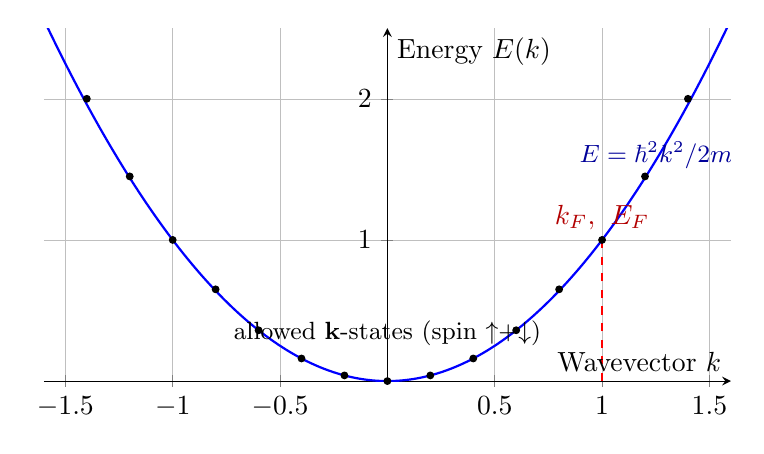
\begin{tikzpicture}
\begin{axis}[
    width=0.85\textwidth,
    height=0.5\textwidth,
    xlabel={Wavevector $k$},
    ylabel={Energy $E(k)$},
    xmin=-1.6, xmax=1.6,
    ymin=0, ymax=2.5,
    grid=both,
    grid style={line width=.1pt, draw=gray!20},
    major grid style={line width=.2pt,draw=gray!50},
    axis lines=middle,
    samples=200,
]
% Parabola
\addplot[blue, thick, domain=-1.6:1.6] {x^2};
\node[anchor=west, blue!60!black, font=\small] at (axis cs:0.85, 1.6) {$E=\hbar^2k^2/2m_e$};

% Allowed k lattice points
\addplot[only marks, mark=*, mark size=1.2pt, black] coordinates {
    (-1.4,2) (-1.2,1.45) (-1.0,1.0) (-0.8,0.65) (-0.6,0.36) (-0.4,0.16) (-0.2,0.04)
    (0.0,0) (0.2,0.04) (0.4,0.16) (0.6,0.36) (0.8,0.65) (1.0,1.0) (1.2,1.45) (1.4,2)
};
\node[anchor=south, font=\small] at (axis cs:0.0, 0.18) {allowed $\vb{k}$-states (spin $\uparrow$+$\downarrow$)};

% kF marker
\addplot[red, dashed, thick] coordinates {(1.0, 0) (1.0, 1.0)};
\node[anchor=south, red!70!black, font=\bfseries] at (axis cs:1.0, 1.0) {$k_F,\ E_F$};
\end{axis}
\end{tikzpicture}
\caption{Free-electron dispersion $E(k)=\hbar^2k^2/2m_e$ as a function of one component of $\vb{k}$ (1D cut). Dots: allowed $\vb{k}$-values from periodic boundary conditions on a length $L$. Vertical line: Fermi wavevector $k_F$ that bounds the occupied states at $T=0$.}
\label{fig:dispersion}
\end{figure}

\begin{figure}[h]
\centering
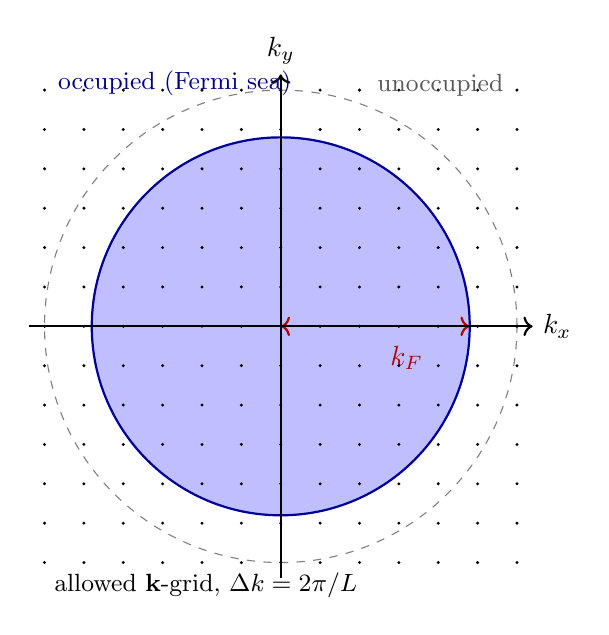
\begin{tikzpicture}
% Filled Fermi disk
\filldraw[blue!25, draw=blue!60!black, thick] (0,0) circle (2.4);
% Outer guide circle
\draw[dashed, gray] (0,0) circle (3.0);
% kF radius arrow
\draw[<->, thick, red!70!black] (0,0) -- (2.4,0);
\node[red!70!black, font=\bfseries] at (1.6, -0.4) {$k_F$};
% Axes
\draw[->, thick] (-3.2,0) -- (3.2,0) node[right] {$k_x$};
\draw[->, thick] (0,-3.2) -- (0,3.2) node[above] {$k_y$};
% Lattice points
\foreach \x in {-3,-2.5,...,3}{
    \foreach \y in {-3,-2.5,...,3}{
        \fill[black] (\x,\y) circle (0.6pt);
    }
}
% Labels
\node[anchor=north west, font=\small] at (-3.0, -3.0) {allowed $\vb{k}$-grid, $\Delta k=2\pi/L$};
\node[anchor=south west, font=\small, blue!50!black] at (-2.95, 2.8) {occupied (Fermi sea)};
\node[anchor=south east, font=\small, gray!70!black] at (2.95, 2.8) {unoccupied};
\end{tikzpicture}
\caption{Filled Fermi sphere in $\vb{k}$-space at $T=0$. Each $\vb{k}$-point on the cubic lattice (spacing $2\pi/L$) accommodates two electrons (spin up and down). All states inside the sphere of radius $k_F=(3\pi^2 n)^{1/3}$ are filled; all states outside are empty.}
\label{fig:fermi_sphere}
\end{figure}

\begin{takeawaybox}{The Extreme Quantum Nature of Metals at Room Temperature}
For typical metals, the Fermi energy is on the order of $2\text{--}12\ \mathrm{eV}$. Translating this into temperature units via $T_F = E_F/k_B$ gives:
\[
T_F \approx \frac{(5\ \mathrm{eV})(1.602 \times 10^{-19}\ \mathrm{J/eV})}{1.381 \times 10^{-23}\ \mathrm{J/K}} \sim 50{,}000\text{--}100{,}000\ \mathrm{K}!
\]
Because ambient temperatures ($T_{\mathrm{room}} \approx 300\ \mathrm{K}$) are orders of magnitude smaller than $T_F$, the ratio $T/T_F \sim 10^{-2} \ll 1$. 

Consequently, conduction electrons in metals at room temperature are in the \textbf{deeply degenerate quantum regime}. Classical Boltzmann statistics is wholly inapplicable; the electron gas is frozen into its quantum ground state with only a minute thermal skin of thickness $\sim k_B T$ excited at the Fermi boundary.
\end{takeawaybox}

\subsection{Empirical Electron Density Formula and Reference Metal Data}
For any elemental metal with mass density $\rho_m$ ($\mathrm{kg/m^3}$), molar mass $A$ ($\mathrm{kg/mol}$), and valence $Z_v$ (number of conduction electrons contributed per atom), the conduction electron density $n$ is calculated from Avogadro's number $N_A \approx 6.022 \times 10^{23}\ \mathrm{mol}^{-1}$ as:
\begin{equation}
\boxed{n = \frac{Z_v N_A \rho_m}{A}}
\label{eq:empirical_n_formula}
\end{equation}
Alternatively, for cubic crystals with lattice constant $a$ and $N_c$ atoms per primitive unit cell:
\begin{equation}
n = \frac{Z_v N_c}{a^3}
\label{eq:lattice_n_formula}
\end{equation}
where $N_c = 1$ for simple cubic, $N_c = 2$ for body-centered cubic (BCC), and $N_c = 4$ for face-centered cubic (FCC) unit cells.

\begin{table}[ht]
\centering
\small
\renewcommand{\arraystretch}{1.25}
\begin{tabular}{lcccccc}
\toprule
\textbf{Element} & \textbf{Valence} $Z_v$ & \textbf{Density} $n$ ($10^{28}\ \mathrm{m}^{-3}$) & $k_F$ ($10^9\ \mathrm{m}^{-1}$) & $E_F$ (eV) & $v_F$ ($10^6\ \mathrm{m/s}$) & $T_F$ ($10^4\ \mathrm{K}$) \\
\midrule
\textbf{Lithium (Li)}   & 1 & 4.70 & 11.2 & 4.74 & 1.29 & 5.51 \\
\textbf{Sodium (Na)}    & 1 & 2.65 & 9.22 & 3.24 & 1.07 & 3.77 \\
\textbf{Potassium (K)}  & 1 & 1.40 & 7.46 & 2.12 & 0.86 & 2.46 \\
\textbf{Copper (Cu)}    & 1 & 8.47 & 13.6 & 7.00 & 1.57 & 8.16 \\
\textbf{Silver (Ag)}    & 1 & 5.86 & 12.0 & 5.49 & 1.39 & 6.38 \\
\textbf{Gold (Au)}      & 1 & 5.90 & 12.1 & 5.53 & 1.40 & 6.42 \\
\textbf{Aluminum (Al)}  & 3 & 18.1 & 17.5 & 11.7 & 2.03 & 13.6 \\
\bottomrule
\end{tabular}
\caption{Conduction electron density and calculated Sommerfeld Fermi parameters for selected elemental metals.}
\label{tab:metal_fermi_params}
\end{table}

\begin{methodbox}{Calculating Conduction Electron Density from Crystallographic Data}
When given crystallographic data instead of macroscopic density:
\begin{enumerate}
    \item Identify the Bravais lattice: Simple Cubic ($1\ \text{atom/cell}$), BCC ($2\ \text{atoms/cell}$), FCC ($4\ \text{atoms/cell}$).
    \item Determine valence $Z_v$: Alkali metals (Li, Na, K) have $Z_v = 1$; Noble metals (Cu, Ag, Au) have $Z_v = 1$; Divalent metals (Be, Mg, Zn) have $Z_v = 2$; Trivalent metals (Al, Ga, In) have $Z_v = 3$.
    \item Compute unit cell volume $V_{\mathrm{cell}} = a^3$ in $\mathrm{m}^3$.
    \item Compute electron density $n = \frac{Z_v N_{\mathrm{atoms}}}{a^3}$.
    \item Use $k_F = (3\pi^2 n)^{1/3}$ and $E_F = \frac{\hbar^2 k_F^2}{2m_e}$ to find all remaining parameters.
\end{enumerate}
\end{methodbox}

\vspace{0.4cm}

% -------------------------------------------------------------------------
% SOLVED EXAMPLES FOR CHAPTER 2
% -------------------------------------------------------------------------
\begin{examplebox}{Fermi Energy and Electron Density of Sodium from Mass Density}{ex:na_fermi}
\textbf{Problem Statement:}
Metallic sodium has mass density $\rho_m = 970\ \mathrm{kg/m^3}$ and atomic weight $A = 23.0\ \mathrm{g/mol} = 23.0 \times 10^{-3}\ \mathrm{kg/mol}$. Sodium is monovalent ($Z_v = 1$). 
Calculate:
\begin{enumerate}[label=(\alph*)]
    \item The conduction electron density $n$.
    \item The Fermi wavevector $k_F$.
    \item The Fermi energy $E_F$ in Joules and in electron-volts.
    \item The Fermi velocity $v_F$ and Fermi temperature $T_F$.
\end{enumerate}

\vspace{0.2cm}\hrule\vspace{0.2cm}
\textbf{Step-by-Step Solution:}

\textbf{(a) Conduction electron concentration $n$:}
Using equation~\eqref{eq:empirical_n_formula}:
\begin{align*}
n &= \frac{Z_v N_A \rho_m}{A} = \frac{(1)(6.022 \times 10^{23}\ \mathrm{mol^{-1}})(970\ \mathrm{kg/m^3})}{23.0 \times 10^{-3}\ \mathrm{kg/mol}} \\
&= \frac{5.841 \times 10^{26}}{2.30 \times 10^{-2}} \approx \mathbf{2.54 \times 10^{28}\ \mathrm{electrons/m^3}}
\end{align*}

\textbf{(b) Fermi wavevector $k_F$:}
\begin{align*}
k_F &= (3\pi^2 n)^{1/3} = \left[ 3\pi^2 (2.54 \times 10^{28}\ \mathrm{m^{-3}}) \right]^{1/3} \\
&= (7.521 \times 10^{29})^{1/3} \approx \mathbf{9.09 \times 10^9\ \mathrm{m^{-1}}} = 0.909\ \text{\AA}^{-1}
\end{align*}

\textbf{(c) Fermi energy $E_F$:}
\begin{align*}
E_F &= \frac{\hbar^2 k_F^2}{2m_e} = \frac{(1.0546 \times 10^{-34}\ \mathrm{J\cdot s})^2 (9.094 \times 10^9\ \mathrm{m^{-1}})^2}{2(9.109 \times 10^{-31}\ \mathrm{kg})} \\
&= \frac{(1.112 \times 10^{-68})(8.270 \times 10^{19})}{1.822 \times 10^{-30}} = \frac{9.196 \times 10^{-49}}{1.822 \times 10^{-30}} \approx \mathbf{5.05 \times 10^{-19}\ \mathrm{J}}
\end{align*}
Converting to electron-volts:
\[
E_F = \frac{5.05 \times 10^{-19}\ \mathrm{J}}{1.6022 \times 10^{-19}\ \mathrm{J/eV}} \approx \mathbf{3.15\ \mathrm{eV}}
\]

\textbf{(d) Fermi velocity $v_F$ and Fermi temperature $T_F$:}
\begin{align*}
v_F &= \frac{\hbar k_F}{m_e} = \frac{(1.0546 \times 10^{-34}\ \mathrm{J\cdot s})(9.094 \times 10^9\ \mathrm{m^{-1}})}{9.109 \times 10^{-31}\ \mathrm{kg}} \approx \mathbf{1.05 \times 10^6\ \mathrm{m/s}} \\
T_F &= \frac{E_F}{k_B} = \frac{5.05 \times 10^{-19}\ \mathrm{J}}{1.3807 \times 10^{-23}\ \mathrm{J/K}} \approx \mathbf{3.66 \times 10^4\ \mathrm{K}} \approx 36{,}600\ \mathrm{K}
\end{align*}
\end{examplebox}

\vspace{0.4cm}

\begin{examplebox}{Fermi Sphere Parameters of Silver from FCC Lattice Constant}{ex:ag_fermi}
\textbf{Problem Statement:}
Silver (Ag) crystallizes in a face-centered cubic (FCC) lattice with lattice constant $a = 4.09\ \text{\AA} = 4.09 \times 10^{-10}\ \mathrm{m}$. Each silver atom contributes $1$ conduction electron ($Z_v = 1$). Calculate:
\begin{enumerate}[label=(\alph*)]
    \item The conduction electron concentration $n$.
    \item The Fermi wavevector $k_F$ and Fermi momentum $p_F$.
    \item The Fermi energy $E_F$ in eV.
    \item The Fermi velocity $v_F$ and Fermi temperature $T_F$.
\end{enumerate}

\vspace{0.2cm}\hrule\vspace{0.2cm}
\textbf{Step-by-Step Solution:}

\textbf{(a) Electron concentration $n$:}
An FCC unit cell contains $4$ atoms ($8 \times \frac{1}{8} + 6 \times \frac{1}{2} = 4$). The unit cell volume is $V_{\mathrm{cell}} = a^3$:
\begin{align*}
V_{\mathrm{cell}} &= (4.09 \times 10^{-10}\ \mathrm{m})^3 \approx 6.842 \times 10^{-29}\ \mathrm{m}^3 \\
n &= \frac{Z_v \times 4}{a^3} = \frac{4}{6.842 \times 10^{-29}\ \mathrm{m}^3} \approx \mathbf{5.85 \times 10^{28}\ \mathrm{m}^{-3}}
\end{align*}

\textbf{(b) Fermi wavevector $k_F$ and momentum $p_F$:}
\begin{align*}
k_F &= (3\pi^2 n)^{1/3} = [3\pi^2 (5.846 \times 10^{28})]^{1/3} = (1.731 \times 10^{30})^{1/3} \approx \mathbf{1.20 \times 10^{10}\ \mathrm{m^{-1}}} = 1.20\ \text{\AA}^{-1} \\
p_F &= \hbar k_F = (1.0546 \times 10^{-34}\ \mathrm{J\cdot s})(1.201 \times 10^{10}\ \mathrm{m^{-1}}) \approx \mathbf{1.27 \times 10^{-24}\ \mathrm{kg\cdot m/s}}
\end{align*}

\textbf{(c) Fermi energy $E_F$:}
\begin{align*}
E_F &= \frac{\hbar^2 k_F^2}{2m_e} = \frac{(1.0546 \times 10^{-34})^2 (1.201 \times 10^{10})^2}{2(9.109 \times 10^{-31})} = \frac{1.604 \times 10^{-48}}{1.822 \times 10^{-30}} \approx 8.798 \times 10^{-19}\ \mathrm{J} \\
E_F &= \frac{8.798 \times 10^{-19}\ \mathrm{J}}{1.6022 \times 10^{-19}\ \mathrm{J/eV}} \approx \mathbf{5.49\ \mathrm{eV}}
\end{align*}

\textbf{(d) Fermi velocity and temperature:}
\begin{align*}
v_F &= \frac{\hbar k_F}{m_e} = \frac{1.266 \times 10^{-24}\ \mathrm{kg\cdot m/s}}{9.109 \times 10^{-31}\ \mathrm{kg}} \approx \mathbf{1.39 \times 10^6\ \mathrm{m/s}} \\
T_F &= \frac{E_F}{k_B} = \frac{8.798 \times 10^{-19}\ \mathrm{J}}{1.3807 \times 10^{-23}\ \mathrm{J/K}} \approx \mathbf{6.37 \times 10^4\ \mathrm{K}} \approx 63{,}700\ \mathrm{K}
\end{align*}
\end{examplebox}

\clearpage


% =========================================================================
% CHAPTER 3: DENSITY OF STATES & GROUND STATE PROPERTIES
% =========================================================================
\section{Density of States and Ground State Properties}
\label{sec:density_of_states}

\subsection{Definition and Significance of the Density of States}
In statistical mechanics and condensed matter physics, the \textbf{Density of States} (DOS), denoted $g(E)$, represents the number of available single-particle quantum states per unit energy interval around energy $E$:
\begin{equation}
g(E) \equiv \frac{dN(E)}{dE}
\label{eq:dos_definition}
\end{equation}
where $N(E)$ is the cumulative number of quantum states with energy less than or equal to $E$. The density of states per unit volume of the specimen is denoted $D(E) \equiv g(E)/V$. 

The DOS is the foundational bridge between microscopic single-particle eigenvalues $E(\vb{k})$ and macroscopic thermodynamic properties. Any thermodynamic average of a physical quantity $A(E)$ can be evaluated as an energy integral:
\begin{equation}
\langle A \rangle = \int_0^\infty A(E) g(E) f(E)\,dE
\end{equation}
where $f(E)$ is the Fermi--Dirac distribution function.

\subsection{Dual Derivations of the 3D Density of States}
We present two complementary, rigorous derivations of the density of states for a three-dimensional free electron gas.

\subsubsection{Method 1: Phase-Space Cell Quantization (Heisenberg Cells)}
According to the quantum correspondence principle and Heisenberg's uncertainty principle ($\Delta x \Delta p_x \ge h$), a single quantum state occupies an elementary volume of $h^3$ in the six-dimensional classical phase space $(\vb{r}, \vb{p})$.

For a spatial volume $V = \iiint d^3r$, the phase-space volume corresponding to electrons with momentum magnitude between $p$ and $p+dp$ is given by the spherical shell in momentum space:
\begin{equation}
d\Omega_{\mathrm{phase}} = V \times 4\pi p^2 dp
\end{equation}
Dividing by the elementary quantum volume $h^3$ and multiplying by the electron spin degeneracy $g_s = 2$ ($m_s = \pm 1/2$), the number of quantum states $g(p)dp$ in the momentum interval $[p, p+dp]$ is:
\begin{equation}
g(p)dp = 2 \times \frac{V \cdot 4\pi p^2 dp}{h^3} = \frac{8\pi V}{h^3} p^2 dp
\label{eq:momentum_dos}
\end{equation}
For non-relativistic free electrons, energy and momentum are related by $E = \frac{p^2}{2m_e} \implies p = \sqrt{2m_e E}$, with differential:
\begin{equation}
dp = \frac{m_e}{\sqrt{2m_e E}}dE = \sqrt{\frac{m_e}{2E}}dE \implies p^2 dp = (2m_e E)\sqrt{\frac{m_e}{2E}}dE = m_e\sqrt{2m_e E}\,dE
\end{equation}
Substituting into equation~\eqref{eq:momentum_dos} and using $h = 2\pi\hbar$:
\begin{equation}
g(E)dE = \frac{8\pi V}{(2\pi\hbar)^3} m_e \sqrt{2m_e E}\,dE = \frac{8\pi V}{8\pi^3\hbar^3} \sqrt{2} m_e^{3/2} E^{1/2} dE
\end{equation}
Simplifying yields the celebrated 3D density of states:
\begin{equation}
\boxed{g(E) = \frac{V}{2\pi^2}\left(\frac{2m_e}{\hbar^2}\right)^{3/2} E^{1/2}}
\label{eq:3d_dos}
\end{equation}

\subsubsection{Method 2: Periodic Boundary Conditions in $k$-Space}
In reciprocal space, the total number of orbital states inside a sphere of radius $k$ is the sphere volume divided by the cell volume per state $(2\pi/L)^3 = 8\pi^3/V$. Multiplying by spin degeneracy $g_s = 2$:
\begin{equation}
N(k) = 2 \times \frac{\frac{4}{3}\pi k^3}{\frac{8\pi^3}{V}} = \frac{V}{3\pi^2}k^3
\label{eq:N_k_sphere}
\end{equation}
Expressing $k$ in terms of energy $E = \frac{\hbar^2 k^2}{2m_e} \implies k = \left(\frac{2m_e E}{\hbar^2}\right)^{1/2}$:
\begin{equation}
N(E) = \frac{V}{3\pi^2}\left(\frac{2m_e E}{\hbar^2}\right)^{3/2} = \frac{V}{3\pi^2}\left(\frac{2m_e}{\hbar^2}\right)^{3/2} E^{3/2}
\label{eq:cumulative_N_E}
\end{equation}
Differentiating with respect to $E$:
\begin{equation}
g(E) = \frac{dN(E)}{dE} = \frac{V}{3\pi^2}\left(\frac{2m_e}{\hbar^2}\right)^{3/2} \left(\frac{3}{2}E^{1/2}\right) = \frac{V}{2\pi^2}\left(\frac{2m_e}{\hbar^2}\right)^{3/2} E^{1/2}
\end{equation}
Both derivations yield identically equation~\eqref{eq:3d_dos}.

\subsection{Dimensionality Comparison: 1D, 2D, and 3D Systems}
The power-law dependence of the electronic density of states on energy depends fundamentally on the spatial dimensionality $d$ of the conductor:
\begin{enumerate}[leftmargin=*]
    \item \textbf{One-Dimensional Conductor (Quantum Wire)}: A wire of length $L$ with $k$-state spacing $\Delta k = 2\pi/L$. State count up to $k$: $N(k) = 2 \times \frac{2k}{2\pi/L} = \frac{2Lk}{\pi}$.
    Using $k = \sqrt{2m_e E}/\hbar$:
    \begin{equation}
    g_{\mathrm{1D}}(E) = \frac{dN}{dE} = \frac{L}{\pi}\sqrt{\frac{2m_e}{\hbar^2}}E^{-1/2} \propto E^{-1/2}
    \label{eq:1d_dos}
    \end{equation}
    The $E^{-1/2}$ divergence as $E \to 0$ is a classic one-dimensional \textbf{Van Hove singularity}.
    \item \textbf{Two-Dimensional Conductor (Quantum Well / 2DEG)}: A quantum well of area $A = L^2$ with $k$-space cell area $(2\pi/L)^2 = 4\pi^2/A$. State count inside a circle of radius $k$:
    $N(k) = 2 \times \frac{\pi k^2}{4\pi^2/A} = \frac{A k^2}{2\pi}$.
    Using $k^2 = \frac{2m_e E}{\hbar^2}$:
    \begin{equation}
    N(E) = \frac{A m_e E}{\pi\hbar^2} \implies \boxed{g_{\mathrm{2D}}(E) = \frac{dN}{dE} = \frac{A m_e}{\pi\hbar^2} = \mathrm{constant}}
    \label{eq:2d_dos}
    \end{equation}
    The 2D density of states is strictly \textbf{energy-independent}!
    \item \textbf{Three-Dimensional Conductor (Bulk Metal)}:
    \begin{equation}
    g_{\mathrm{3D}}(E) \propto E^{1/2}
    \end{equation}
\end{enumerate}

\begin{figure}[h]
\centering
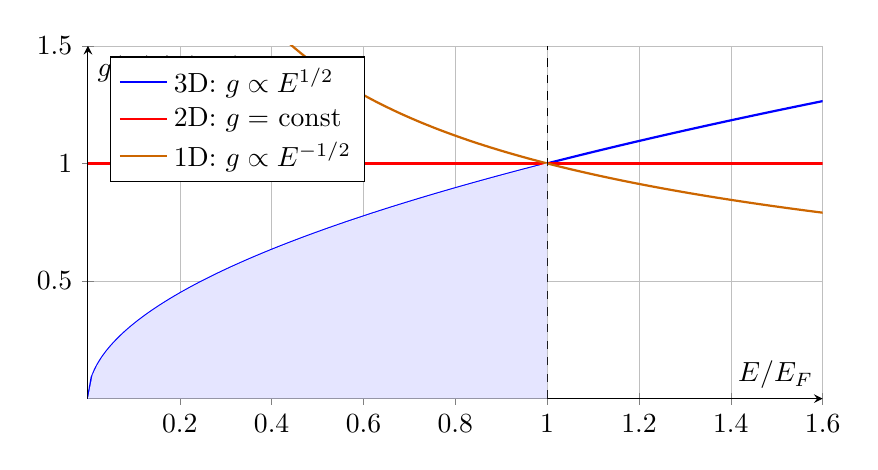
\begin{tikzpicture}
\begin{axis}[
    width=0.9\textwidth,
    height=0.5\textwidth,
    xlabel={$E/E_F$},
    ylabel={$g(E)/g(E_F)$},
    xmin=0, xmax=1.6,
    ymin=0, ymax=1.5,
    legend pos=north west,
    legend cell align=left,
    grid=both,
    grid style={line width=.1pt, draw=gray!20},
    major grid style={line width=.2pt,draw=gray!50},
    axis lines=middle,
    samples=200,
]
% 3D: sqrt(E) -> normalized to (E/EF)^(1/2)
\addplot[blue, thick, domain=0:1.6] {sqrt(x)};
\addlegendentry{3D: $g\propto E^{1/2}$}

% 2D: const
\addplot[red, thick, domain=0:1.6] {1};
\addlegendentry{2D: $g=$ const}

% 1D: 1/sqrt(E)
\addplot[orange!80!black, thick, domain=0.02:1.6] {1/sqrt(x)};
\addlegendentry{1D: $g\propto E^{-1/2}$}

% Fermi level line (after legend so it overlays cleanly)
\addplot[black, dashed] coordinates {(1,0) (1,1.5)};
\node[anchor=south, font=\bfseries] at (axis cs:1, 1.5) {$E_F$};

% Shaded occupied region for 3D
\addplot[blue, fill=blue!10, draw=none, domain=0:1, samples=100] {sqrt(x)} \closedcycle;
\end{axis}
\end{tikzpicture}
\caption{Comparison of the free-electron density of states in 1D, 2D, and 3D, each normalized to $g(E_F)$ at $E=E_F$. The 3D DOS grows as $E^{1/2}$, the 2D DOS is constant, and the 1D DOS diverges as $E^{-1/2}$ at the band edge. The shaded area shows the 3D occupied states at $T=0$.}
\label{fig:dos}
\end{figure}

\begin{checkpointbox}{Why is the 2D Density of States Energy-Independent?}
In $d$ spatial dimensions with parabolic dispersion $E \propto k^2$, the $k$-space volume scales as $k^d \propto E^{d/2}$. The cumulative state count is $N(E) \propto E^{d/2}$, and differentiating gives the density of states:
\[
g(E) = \frac{dN}{dE} \propto E^{\frac{d}{2} - 1}
\]
\begin{itemize}
    \item For $d=1$: $g(E) \propto E^{-1/2}$ (decreases with energy).
    \item For $d=2$: $g(E) \propto E^0 = \text{constant}$ (flat step-like spectrum).
    \item For $d=3$: $g(E) \propto E^{1/2}$ (increases monotonically with energy).
\end{itemize}
The energy-independent density of states in 2D systems is of enormous practical significance in semiconductor physics: it creates sharp, step-like absorption spectra in GaAs/AlGaAs quantum wells, enabling low-threshold semiconductor quantum-well lasers and high-frequency HEMTs.
\end{checkpointbox}

\subsection{Volumetric Density of States and Values at the Fermi Level}
Dividing equation~\eqref{eq:3d_dos} by volume $V$ gives the density of states per unit volume:
\begin{equation}
D(E) \equiv \frac{g(E)}{V} = \frac{1}{2\pi^2}\left(\frac{2m_e}{\hbar^2}\right)^{3/2} E^{1/2}
\label{eq:volumetric_dos}
\end{equation}
This can be expressed in an exceptionally compact, intuitive form using the Fermi energy $E_F = \frac{\hbar^2}{2m_e}(3\pi^2 n)^{2/3} \implies n = \frac{1}{3\pi^2}\left(\frac{2m_e E_F}{\hbar^2}\right)^{3/2}$:
\begin{equation}
\boxed{D(E) = \frac{3n}{2E_F}\left(\frac{E}{E_F}\right)^{1/2}}
\label{eq:dos_normalized}
\end{equation}
Evaluating this directly at the Fermi level $E = E_F$:
\begin{equation}
\boxed{D(E_F) = \frac{3n}{2E_F}} \quad \text{and} \quad \boxed{g(E_F) = \frac{3N}{2E_F}}
\label{eq:dos_at_Ef}
\end{equation}
This beautiful relationship states that the density of states at $E_F$ is exactly $1.5$ times the average density of states $n/E_F$ across the entire occupied band!

\subsection{Ground-State Internal Energy at Absolute Zero}
At $T = 0\ \mathrm{K}$, all single-particle states up to $E_F$ are filled with probability $f(E) = 1$, and all states above $E_F$ are empty ($f(E) = 0$). The total internal energy $U_0$ of the electron gas is obtained by integrating the energy times the density of states:
\begin{equation}
U_0 = \int_0^{E_F} E\,g(E)\,dE = \int_0^{E_F} E \left[ \frac{3N}{2E_F^{3/2}} E^{1/2} \right] dE = \frac{3N}{2E_F^{3/2}} \int_0^{E_F} E^{3/2}\,dE
\end{equation}
Evaluating the integral:
\begin{equation}
\int_0^{E_F} E^{3/2}\,dE = \frac{2}{5}E_F^{5/2}
\end{equation}
Substituting back:
\begin{equation}
U_0 = \frac{3N}{2E_F^{3/2}} \left(\frac{2}{5}E_F^{5/2}\right) = \frac{3}{5}N E_F
\label{eq:ground_state_energy}
\end{equation}
The average kinetic energy per electron in the ground state is therefore:
\begin{equation}
\boxed{\langle E \rangle_0 = \frac{U_0}{N} = \frac{3}{5}E_F}
\label{eq:average_energy_zero_T}
\end{equation}
Even at absolute zero, quantum confinement and Pauli exclusion force electrons to possess significant kinetic energy: for copper ($E_F = 7.0\ \mathrm{eV}$), the mean zero-point energy is $\langle E \rangle_0 = 4.2\ \mathrm{eV}$ per electron, corresponding to an effective classical thermal temperature of $\frac{2}{3}\langle E \rangle_0 / k_B \approx 32{,}000\ \mathrm{K}$!

\subsection{Thermodynamic Degeneracy Pressure and Electronic Bulk Modulus}
From fundamental thermodynamics, the pressure exerted by a quantum gas at $T = 0\ \mathrm{K}$ is defined by the volume derivative of its ground-state internal energy at constant particle number:
\begin{equation}
P_0 = -\left(\frac{\partial U_0}{\partial V}\right)_N
\label{eq:pressure_thermo_def}
\end{equation}
Using $U_0 = \frac{3}{5}N E_F$, the volume dependence enters entirely through $E_F$:
\begin{equation}
E_F = \frac{\hbar^2}{2m_e}\left(3\pi^2 \frac{N}{V}\right)^{2/3} \propto V^{-2/3}
\end{equation}
Differentiating with respect to $V$:
\begin{equation}
\frac{dE_F}{dV} = -\frac{2}{3}\frac{E_F}{V}
\end{equation}
Substituting this into equation~\eqref{eq:pressure_thermo_def}:
\begin{equation}
P_0 = -\frac{3}{5}N \left(-\frac{2}{3}\frac{E_F}{V}\right) = \frac{2}{5}\left(\frac{N}{V}\right)E_F
\end{equation}
We obtain the fundamental \textbf{electron degeneracy pressure}:
\begin{equation}
\boxed{P_0 = \frac{2}{5}n E_F}
\label{eq:fermi_pressure}
\end{equation}
Since $U_0/V = \frac{3}{5}n E_F$, the degeneracy pressure is related to the internal energy density by:
\begin{equation}
P_0 = \frac{2}{3}\left(\frac{U_0}{V}\right)
\label{eq:pressure_energy_relation}
\end{equation}
The mechanical resistance of the electron gas to isotropic compression is quantified by the \textbf{bulk modulus} $B$:
\begin{equation}
B \equiv -V\left(\frac{\partial P}{\partial V}\right)_N
\label{eq:bulk_modulus_def}
\end{equation}
Since $P_0 \propto n E_F \propto V^{-1} V^{-2/3} = V^{-5/3}$, differentiating gives:
\begin{equation}
\frac{\partial P_0}{\partial V} = -\frac{5}{3}\frac{P_0}{V}
\end{equation}
Substituting into equation~\eqref{eq:bulk_modulus_def} yields:
\begin{equation}
\boxed{B = \frac{5}{3}P_0 = \frac{2}{3}n E_F}
\label{eq:bulk_modulus}
\end{equation}

\begin{takeawaybox}{Fermi Degeneracy Pressure and Stellar Stability}
The degeneracy pressure $P_0 = \frac{2}{5}n E_F$ is a purely quantum kinetic phenomenon. It does not arise from electrostatic Coulomb repulsion, but from the Heisenberg uncertainty principle and Pauli exclusion: compressing the gas forces electrons into smaller spatial regions, increasing their quantum zero-point momenta and kinetic energies.

In astrophysics, this non-thermal electron degeneracy pressure is precisely the cosmic force that prevents \textbf{white dwarf stars} (such as Sirius B) from collapsing under their enormous gravitational self-attraction. When a star's core exhausts its nuclear fuel, electron degeneracy pressure supports the star against gravity up to the Chandrasekhar mass limit ($M \approx 1.44 M_\odot$).
\end{takeawaybox}

\vspace{0.4cm}

% -------------------------------------------------------------------------
% SOLVED EXAMPLES FOR CHAPTER 3
% -------------------------------------------------------------------------
\begin{examplebox}{Degeneracy Pressure and Bulk Modulus of Metallic Copper}{ex:copper_pressure}
\textbf{Problem Statement:}
For metallic copper at $T = 0\ \mathrm{K}$, the conduction electron density is $n = 8.47 \times 10^{28}\ \mathrm{m}^{-3}$ and the Fermi energy is $E_F = 7.00\ \mathrm{eV}$.
\begin{enumerate}[label=(\alph*)]
    \item Calculate the zero-point internal energy density $u_0 = U_0/V$ in $\mathrm{J/m^3}$.
    \item Determine the quantum degeneracy pressure $P_0$ in Pascals ($\mathrm{N/m^2}$) and in atmospheres ($1\ \mathrm{atm} \approx 1.013 \times 10^5\ \mathrm{Pa}$).
    \item Compute the electronic bulk modulus $B$ of copper, and compare it with the measured macroscopic bulk modulus of copper ($B_{\mathrm{exp}} \approx 13.7 \times 10^{10}\ \mathrm{Pa}$).
\end{enumerate}

\vspace{0.2cm}\hrule\vspace{0.2cm}
\textbf{Step-by-Step Solution:}

\textbf{(a) Zero-point energy density $u_0$:}
First convert $E_F$ to Joules:
\[
E_F = (7.00\ \mathrm{eV})(1.6022 \times 10^{-19}\ \mathrm{J/eV}) = 1.1215 \times 10^{-18}\ \mathrm{J}
\]
The energy density is:
\begin{align*}
u_0 &= \frac{3}{5}n E_F = \frac{3}{5}(8.47 \times 10^{28}\ \mathrm{m^{-3}})(1.1215 \times 10^{-18}\ \mathrm{J}) \\
&= (5.082 \times 10^{28})(1.1215 \times 10^{-18}) \approx \mathbf{5.70 \times 10^{10}\ \mathrm{J/m^3}}
\end{align*}

\textbf{(b) Quantum degeneracy pressure $P_0$:}
Using equation~\eqref{eq:fermi_pressure}:
\begin{align*}
P_0 &= \frac{2}{5}n E_F = \frac{2}{3}u_0 = \frac{2}{3}(5.70 \times 10^{10}\ \mathrm{J/m^3}) \approx \mathbf{3.80 \times 10^{10}\ \mathrm{Pa}}
\end{align*}
Converting to atmospheres:
\[
P_0 = \frac{3.80 \times 10^{10}\ \mathrm{Pa}}{1.01325 \times 10^5\ \mathrm{Pa/atm}} \approx \mathbf{3.75 \times 10^5\ \mathrm{atm}} \approx \mathbf{375{,}000\ \text{atmospheres}!}
\]

\textbf{(c) Electronic bulk modulus $B$:}
Using equation~\eqref{eq:bulk_modulus}:
\[
B = \frac{5}{3}P_0 = \frac{2}{3}n E_F = u_0 \approx \mathbf{5.70 \times 10^{10}\ \mathrm{Pa}} = 57.0\ \mathrm{GPa}
\]
\textbf{Comparison:} The experimental bulk modulus of copper is $B_{\mathrm{exp}} \approx 137\ \mathrm{GPa}$. The free electron gas accounts for:
\[
\frac{B_{\mathrm{electronic}}}{B_{\mathrm{exp}}} = \frac{57.0\ \mathrm{GPa}}{137\ \mathrm{GPa}} \approx \mathbf{41.6\%}
\]
Over $40\%$ of the macroscopic mechanical stiffness of metallic copper originates purely from quantum electron degeneracy pressure! The remainder arises from ion core Coulomb repulsions and exchange-correlation forces.
\end{examplebox}

\vspace{0.4cm}

\begin{examplebox}{Thermally Active Fraction of Conduction Electrons at Room Temperature}{ex:thermal_fraction}
\textbf{Problem Statement:}
Consider conduction electrons in metallic copper ($E_F = 7.00\ \mathrm{eV}$) at room temperature ($T = 300\ \mathrm{K}$).
\begin{enumerate}[label=(\alph*)]
    \item Evaluate the thermal energy scale $k_B T$ in electron-volts at $300\ \mathrm{K}$.
    \item Estimate the fraction $f_{\mathrm{active}}$ of conduction electrons that lie within an energy window of width $\Delta E = \pm k_B T$ around the Fermi energy.
    \item Compute the number of thermally active electrons in $1.0\ \mathrm{cm}^3$ of metallic copper.
\end{enumerate}

\vspace{0.2cm}\hrule\vspace{0.2cm}
\textbf{Step-by-Step Solution:}

\textbf{(a) Thermal energy scale $k_B T$:}
\[
k_B T = (8.6173 \times 10^{-5}\ \mathrm{eV/K})(300\ \mathrm{K}) \approx \mathbf{0.02585\ \mathrm{eV}} \approx \frac{1}{39}\ \mathrm{eV}
\]

\textbf{(b) Thermally active fraction $f_{\mathrm{active}}$:}
The number of electrons per unit volume residing in an energy strip of width $\Delta E = 2 k_B T$ centered at $E_F$ is approximately:
\[
\Delta n \approx D(E_F) \Delta E = \left(\frac{3n}{2E_F}\right)(2 k_B T) = 3n\left(\frac{k_B T}{E_F}\right)
\]
The active fraction is:
\begin{align*}
f_{\mathrm{active}} &\approx \frac{\Delta n}{n} = 3\left(\frac{k_B T}{E_F}\right) = 3\left(\frac{0.02585\ \mathrm{eV}}{7.00\ \mathrm{eV}}\right) \\
&= 3(3.69 \times 10^{-3}) \approx \mathbf{1.11 \times 10^{-2}} \approx \mathbf{1.1\%}
\end{align*}
(If using the single-sided interval $k_B T/E_F$, the fraction is $0.37\%$).

\textbf{(c) Number of active electrons in $1\ \mathrm{cm}^3$:}
For $V = 1.0\ \mathrm{cm}^3 = 1.0 \times 10^{-6}\ \mathrm{m}^3$, with $n = 8.47 \times 10^{28}\ \mathrm{m}^{-3}$:
\[
N_{\mathrm{total}} = n V = 8.47 \times 10^{22}\ \text{electrons}
\]
The number of thermally active electrons is:
\[
N_{\mathrm{active}} = f_{\mathrm{active}} N_{\mathrm{total}} \approx (0.0111)(8.47 \times 10^{22}) \approx \mathbf{9.4 \times 10^{20}\ \text{electrons}}
\]
\textbf{Physical Meaning:} Over $98.9\%$ of the conduction electrons in copper at room temperature are quantum-mechanically locked in the interior of the Fermi sea and cannot participate in thermal absorption.
\end{examplebox}

\clearpage


% =========================================================================
% CHAPTER 4: QUANTUM STATISTICS & ELECTRONIC HEAT CAPACITY
% =========================================================================
\section{Quantum Statistics and Electronic Heat Capacity}
\label{sec:heat_capacity}

\subsection{The Fermi--Dirac Distribution Function}
Because electrons are identical fermions possessing half-integer spin ($s=1/2$), the probability $f(E)$ that a single-particle quantum state of energy $E$ is occupied in thermal equilibrium at temperature $T$ is governed by the \textbf{Fermi--Dirac distribution}:
\begin{equation}
\boxed{f(E) = \frac{1}{\exp\left(\frac{E-\mu}{k_B T}\right) + 1}}
\label{eq:fd_distribution}
\end{equation}
where $\mu(T)$ is the chemical potential of the electron gas (the Gibbs free energy per particle).

\paragraph{Physical Properties of $f(E)$:}
\begin{itemize}[leftmargin=*]
    \item \textbf{Zero-Temperature Limit} ($T \to 0\ \mathrm{K}$): $\mu(0) \equiv E_F$.
    \begin{equation}
    f(E) = \begin{cases} 1, & E < E_F \\ 0, & E > E_F \end{cases}
    \end{equation}
    The distribution is a pristine unit step function: every single quantum state below $E_F$ is completely occupied, and every state above $E_F$ is completely vacant.
    \item \textbf{Finite Temperatures} ($T > 0\ \mathrm{K}$): The sharp step at $E_F$ becomes smoothed over an energy interval of characteristic width $\sim \pm k_B T$. At $E = \mu(T)$, the occupation probability is identically $1/2$ at all temperatures:
    \begin{equation}
    f(\mu) = \frac{1}{e^0 + 1} = \frac{1}{2}
    \end{equation}
    \item \textbf{Particle-Hole Symmetry}: The probability that an electron occupies a state an energy $\Delta$ above the chemical potential equals the probability that a state an energy $\Delta$ below the chemical potential is unoccupied (vacant hole):
    \begin{equation}
    f(\mu + \Delta) = 1 - f(\mu - \Delta) \iff f(\mu + \Delta) + f(\mu - \Delta) = 1
    \label{eq:particle_hole_sym}
    \end{equation}
\end{itemize}

\begin{figure}[h]
\centering
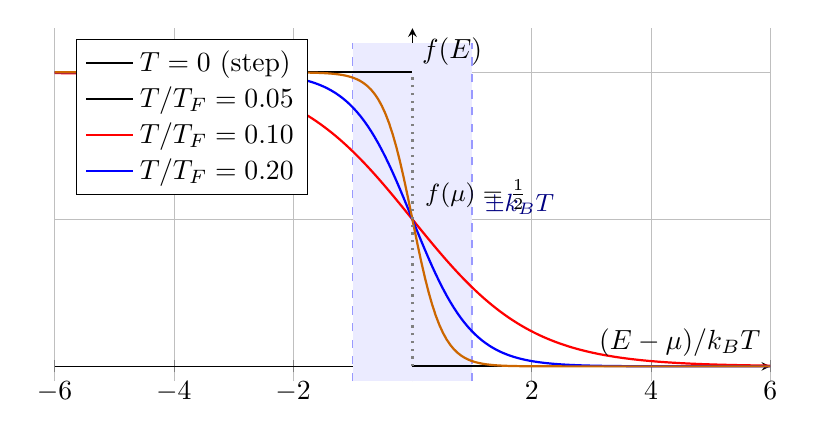
\begin{tikzpicture}
\begin{axis}[
    width=0.88\textwidth,
    height=0.5\textwidth,
    xlabel={$(E-\mu)/k_B T$},
    ylabel={$f(E)$},
    xmin=-6, xmax=6,
    ymin=-0.05, ymax=1.15,
    legend pos=north west,
    legend cell align=left,
    grid=both,
    grid style={line width=.1pt, draw=gray!20},
    major grid style={line width=.2pt,draw=gray!50},
    axis lines=middle,
    samples=200,
]
% k_BT smearing band (shaded)
\fill[blue!8] (axis cs:-1,-0.05) rectangle (axis cs:1,1.1);
\draw[blue!40, dashed] (axis cs:-1,-0.05) -- (axis cs:-1,1.1);
\draw[blue!40, dashed] (axis cs:1,-0.05) -- (axis cs:1,1.1);
\node[anchor=west, blue!50!black, font=\small] at (axis cs:1.05, 0.55) {$\pm k_B T$};

% T = 0 step
\addplot[black, thick, domain=-6:0] {1};
\addplot[black, thick, domain=0:6] {0};
\addlegendentry{$T=0$ (step)}

% Finite-T curves at several T/T_F
\addplot[red, thick, domain=-6:6] {1/(exp(x)+1)};
\addlegendentry{$T/T_F=0.05$}

\addplot[blue, thick, domain=-6:6] {1/(exp(2*x)+1)};
\addlegendentry{$T/T_F=0.10$}

\addplot[orange!80!black, thick, domain=-6:6] {1/(exp(4*x)+1)};
\addlegendentry{$T/T_F=0.20$}

% Reference line f = 1/2 at E = mu
\addplot[gray, dotted, thick] coordinates {(0,0) (0,1)};
\node[anchor=south west, font=\small] at (axis cs:0.05, 0.5) {$f(\mu)=\tfrac{1}{2}$};
\end{axis}
\end{tikzpicture}
\caption{Fermi--Dirac distribution $f(E)$ at $T=0$ (black step) and at finite temperatures, plotted versus $(E-\mu)/k_BT$. The shaded band marks the thermal smearing region of width $\sim \pm k_BT$. Even at $T/T_F\sim 0.1$ (typical room temperature for a metal), the distribution is still an almost perfect step.}
\label{fig:fermi_dirac}
\end{figure}

\subsection{Temperature Dependence of the Chemical Potential}
The total electron density $n$ in a metal is fixed by the positive ionic lattice charges and is independent of temperature. Particle conservation requires:
\begin{equation}
n = \int_0^\infty D(E) f(E)\,dE = \int_0^\infty \frac{3n}{2E_F^{3/2}} \frac{E^{1/2}}{\exp\left(\frac{E-\mu(T)}{k_B T}\right) + 1}\,dE
\label{eq:n_conservation}
\end{equation}
Because the 3D density of states $D(E) \propto E^{1/2}$ increases with energy, the density of states available above $\mu$ is slightly greater than that below $\mu$. To maintain a constant particle count as states above $\mu$ become thermally populated, the chemical potential must shift slightly downward with increasing temperature. 

Evaluating equation~\eqref{eq:n_conservation} via the Sommerfeld expansion yields the temperature dependence of $\mu(T)$:
\begin{equation}
\boxed{\mu(T) \approx E_F \left[ 1 - \frac{\pi^2}{12}\left(\frac{T}{T_F}\right)^2 + \mathcal{O}\left(\left(\frac{T}{T_F}\right)^4\right) \right]}
\label{eq:chemical_potential_T}
\end{equation}
For metallic copper ($T_F \approx 81{,}200\ \mathrm{K}$) at room temperature ($T = 300\ \mathrm{K}$), $(T/T_F)^2 \approx (3.69 \times 10^{-3})^2 \approx 1.36 \times 10^{-5}$. The chemical potential drops by only $0.001\%$! In virtually all solid-state calculations, setting $\mu(T) \approx E_F$ is an extraordinarily accurate approximation.

\subsection{The Classical Electronic Heat Capacity Failure}
According to classical statistical mechanics (the equipartition theorem), each classical degree of freedom possesses an average thermal kinetic energy of $\frac{1}{2}k_B T$. In a three-dimensional gas, the internal thermal energy per mole of electrons should be:
\begin{equation}
U_{\mathrm{classical}} = \frac{3}{2}N_A k_B T = \frac{3}{2}R T
\end{equation}
predicting a constant molar electronic heat capacity:
\begin{equation}
C_{V,\mathrm{classical}} = \frac{\partial U}{\partial T} = \frac{3}{2}R \approx 12.47\ \mathrm{J/(mol\cdot K)}
\label{eq:classical_cv}
\end{equation}
However, 19th-century calorimetric measurements revealed that the total heat capacity of metals at room temperature follows the empirical Dulong--Petit law $C_V \approx 3R \approx 25\ \mathrm{J/(mol\cdot K)}$, which is fully accounted for by lattice vibrations (phonons) alone! 

The conduction electrons appeared to contribute almost \emph{nothing} to the specific heat. Classical physics was utterly powerless to explain why an electron gas capable of conducting massive electrical currents failed to absorb thermal energy.

\subsection{Qualitative Quantum Resolution via the Pauli Principle}
Quantum mechanics provides an elegant, physically transparent resolution:
\begin{enumerate}
    \item When a metal is heated from $0\ \mathrm{K}$ to temperature $T$, thermal fluctuations can transfer energy packets of magnitude $\sim k_B T$ to electrons.
    \item An electron lying at energy $E$ can absorb this thermal quantum only if the target state at $E + k_B T$ is empty.
    \item For an electron situated deep within the Fermi sea (where $E_F - E \gg k_B T$), all adjacent states up to $E + k_B T$ are already $100\%$ occupied by other electrons. The Pauli exclusion principle strictly forbids the transition!
    \item Therefore, \textbf{only electrons in a narrow surface shell} of thickness $\sim k_B T$ around the Fermi level can absorb thermal energy.
\end{enumerate}
The fraction of thermally excited electrons is approximately:
\begin{equation}
f_{\mathrm{excited}} \approx \frac{k_B T}{E_F} = \frac{T}{T_F} \sim 10^{-2}
\end{equation}
Each excited electron absorbs an energy of order $k_B T$. The thermal energy per mole of electrons is:
\begin{equation}
\Delta U \approx N_A \left(\frac{T}{T_F}\right) k_B T = R \frac{T^2}{T_F}
\end{equation}
Differentiating with respect to temperature gives the electronic heat capacity:
\begin{equation}
C_{el} = \frac{d(\Delta U)}{dT} \approx 2 R \left(\frac{T}{T_F}\right) \propto T
\label{eq:cv_qualitative}
\end{equation}
Because $T/T_F \approx 10^{-2}$ at room temperature, the true electronic heat capacity is suppressed by two orders of magnitude relative to classical equipartition, completely solving the mystery!

\begin{checkpointbox}{Why is Electronic Heat Capacity Suppressed by $10^{-2}$?}
The suppression is a direct manifestation of Fermi--Dirac quantum statistics:
\begin{itemize}
    \item In a classical Boltzmann gas, particles are distinguishable; all $N$ particles absorb $\frac{3}{2}k_B T$ equally, producing a constant $C_V = \frac{3}{2}R$.
    \item In a quantum Fermi gas, particles are indistinguishable fermions; Pauli exclusion freezes over $99\%$ of the carriers into inert, inaccessible quantum states.
\end{itemize}
\end{checkpointbox}

\subsection{Rigorous Sommerfeld Expansion and Electronic Heat Capacity}
To evaluate the electronic internal energy rigorously, consider the general thermodynamic integral for any smooth function $\phi(E)$:
\begin{equation}
I = \int_0^\infty \phi(E) f(E)\,dE
\end{equation}
Let $\Phi(E) \equiv \int_0^E \phi(E')\,dE'$. Integrating by parts:
\begin{equation}
I = \Big[ \Phi(E)f(E) \Big]_0^\infty - \int_0^\infty \Phi(E)\frac{\partial f}{\partial E}\,dE = \int_0^\infty \Phi(E)\left(-\frac{\partial f}{\partial E}\right)dE
\label{eq:parts_sommerfeld}
\end{equation}
At low temperatures, $-\frac{\partial f}{\partial E}$ is a sharp symmetric bell curve centered at $E = \mu$ with width $\sim k_B T$. Expanding $\Phi(E)$ in a Taylor series about $E = \mu$:
\begin{equation}
\Phi(E) = \Phi(\mu) + \Phi'(\mu)(E-\mu) + \frac{1}{2}\Phi''(\mu)(E-\mu)^2 + \dots
\end{equation}
Substituting this expansion into equation~\eqref{eq:parts_sommerfeld}:
\begin{equation}
I = \Phi(\mu)\int_0^\infty \left(-\frac{\partial f}{\partial E}\right)dE + \phi(\mu)\int_0^\infty (E-\mu)\left(-\frac{\partial f}{\partial E}\right)dE + \frac{1}{2}\phi'(\mu)\int_0^\infty (E-\mu)^2\left(-\frac{\partial f}{\partial E}\right)dE + \dots
\end{equation}
Using the dimensionless variable $x \equiv \frac{E-\mu}{k_B T}$:
\begin{equation}
-\frac{\partial f}{\partial E} = \frac{1}{k_B T}\frac{e^x}{(e^x+1)^2}
\end{equation}
The three integrals evaluate as follows:
\begin{enumerate}
    \item $\int_{-\infty}^\infty \frac{e^x}{(e^x+1)^2}\,dx = \left[ -\frac{1}{e^x+1} \right]_{-\infty}^\infty = 1$.
    \item $\int_{-\infty}^\infty x \frac{e^x}{(e^x+1)^2}\,dx = 0$ (integrand is strictly odd).
    \item The second-order definite integral:
    \begin{equation}
    \int_{-\infty}^\infty x^2 \frac{e^x}{(e^x+1)^2}\,dx = 2\int_0^\infty x^2 \frac{e^{-x}}{(1+e^{-x})^2}\,dx
    \end{equation}
    Using the binomial series $\frac{e^{-x}}{(1+e^{-x})^2} = \sum_{n=1}^\infty (-1)^{n-1} n e^{-nx}$:
    \begin{align}
    \int_{-\infty}^\infty x^2 \frac{e^x}{(e^x+1)^2}\,dx &= 2\sum_{n=1}^\infty (-1)^{n-1} n \int_0^\infty x^2 e^{-nx}\,dx = 2\sum_{n=1}^\infty (-1)^{n-1} n \left(\frac{2!}{n^3}\right) \nonumber \\
    &= 4\sum_{n=1}^\infty \frac{(-1)^{n-1}}{n^2} = 4\left( \frac{\pi^2}{12} \right) = \frac{\pi^2}{3}
    \label{eq:definite_integral_pi2_3}
    \end{align}
\end{enumerate}
This yields the celebrated \textbf{Sommerfeld Expansion Lemma}:
\begin{equation}
\boxed{\int_0^\infty \phi(E)f(E)\,dE = \int_0^\mu \phi(E)\,dE + \frac{\pi^2}{6}(k_B T)^2 \left.\frac{d\phi}{dE}\right|_{E=\mu} + \mathcal{O}\left((k_B T)^4\right)}
\label{eq:sommerfeld_lemma}
\end{equation}

\paragraph{Application to Internal Energy $U(T)$:}
Setting $\phi(E) = E\,g(E)$:
\begin{equation}
U(T) = \int_0^\mu E\,g(E)\,dE + \frac{\pi^2}{6}(k_B T)^2 \left.\frac{d(E\,g(E))}{dE}\right|_{E=\mu}
\end{equation}
Since $\mu(T) = E_F - \frac{\pi^2}{12}\frac{(k_BT)^2}{E_F}$, the integral $\int_0^\mu E g(E)dE$ evaluates to $U_0 - \frac{\pi^2}{12}(k_BT)^2 g(E_F)$. Combining terms:
\begin{equation}
U(T) = U_0 + \frac{\pi^2}{6}g(E_F)(k_B T)^2
\label{eq:thermal_internal_energy}
\end{equation}
Differentiating with respect to temperature gives the exact \textbf{electronic specific heat}:
\begin{equation}
\boxed{C_{el} = \frac{\partial U}{\partial T} = \frac{\pi^2}{3}g(E_F) k_B^2 T}
\label{eq:c_el_dos}
\end{equation}
Substituting $g(E_F) = \frac{3N}{2E_F} = \frac{3N}{2k_B T_F}$:
\begin{equation}
\boxed{C_{el} = \frac{\pi^2}{2}N k_B \left(\frac{T}{T_F}\right)}
\label{eq:c_el_fermi_temp}
\end{equation}
For one mole of electrons ($N = N_A$, $N_A k_B = R$):
\begin{equation}
\boxed{C_{el} = \gamma T, \quad \text{where} \quad \gamma \equiv \frac{\pi^2}{2}\frac{R k_B}{E_F} = \frac{\pi^2}{3}D(E_F)k_B^2}
\label{eq:sommerfeld_gamma}
\end{equation}
The constant $\gamma$ is known as the \textbf{Sommerfeld coefficient} (or linear electronic specific heat coefficient).

\begin{figure}[h]
\centering
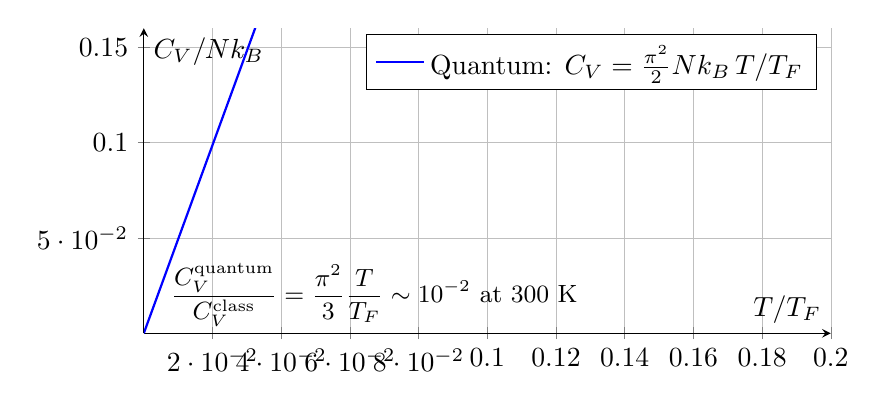
\begin{tikzpicture}
\begin{axis}[
    width=0.85\textwidth,
    height=0.45\textwidth,
    xlabel={$T/T_F$},
    ylabel={$C_V / N k_B$},
    xmin=0, xmax=0.20,
    ymin=0, ymax=0.16,
    grid=both,
    grid style={line width=.1pt, draw=gray!20},
    major grid style={line width=.2pt,draw=gray!50},
    axis lines=middle,
    samples=100,
]
% Quantum (linear) C_V ~ pi^2/2 * T/TF
\addplot[blue, thick, domain=0:0.20] {(pi^2/2)*x};
\addlegendentry{Quantum: $C_V=\tfrac{\pi^2}{2}Nk_B\,T/T_F$}

% Classical (constant) - shown as horizontal line out of range
\addplot[red, dashed, thick] coordinates {(0, 1.5) (0.2, 1.5)};
\node[anchor=south, red!70!black] at (axis cs:0.10, 1.5) {Classical: $\tfrac{3}{2}Nk_B$ (off scale)};

% Ratio annotation
\node[anchor=west, font=\small] at (axis cs:0.005, 0.020) {$\dfrac{C_V^{\rm quantum}}{C_V^{\rm class}}=\dfrac{\pi^2}{3}\dfrac{T}{T_F}\sim 10^{-2}$ at 300 K};
\end{axis}
\end{tikzpicture}
\caption{Linear-in-$T$ electronic specific heat of a free-electron metal (blue) compared with the classical equipartition prediction (red dashed, off scale). The quantum result is smaller by a factor of order $T/T_F\sim 10^{-2}$ at room temperature.}
\label{fig:cv_quantum_vs_classical}
\end{figure}

\subsection{Separation of Electronic and Phonon Heat Capacities}
In a real metallic crystal, the total measured heat capacity at low temperatures ($T \ll \Theta_D$, where $\Theta_D$ is the Debye temperature) is the sum of conduction electron excitations and acoustic lattice vibrations (Debye phonons):
\begin{equation}
C(T) = C_{el} + C_{ph} = \gamma T + \beta T^3
\label{eq:total_heat_capacity}
\end{equation}
where the Debye phonon coefficient $\beta$ is:
\begin{equation}
\beta = \frac{12\pi^4}{5}\frac{N_A k_B}{\Theta_D^3} = \frac{12\pi^4 R}{5\Theta_D^3}
\label{eq:debye_beta}
\end{equation}
To disentangle the linear electronic contribution from the cubic phonon contribution experimentally, equation~\eqref{eq:total_heat_capacity} is divided by $T$:
\begin{equation}
\boxed{\frac{C(T)}{T} = \gamma + \beta T^2}
\label{eq:c_over_t_plot}
\end{equation}
A plot of experimental $C(T)/T$ versus $T^2$ yields a straight line:
\begin{itemize}
    \item The \textbf{vertical intercept} at $T^2 = 0$ gives the Sommerfeld coefficient $\gamma$, directly measuring the electronic density of states at the Fermi energy $g(E_F)$!
    \item The \textbf{slope} of the line gives the Debye coefficient $\beta$, directly yielding the Debye temperature $\Theta_D$.
\end{itemize}
The \textbf{crossover temperature} $T^*$ where electronic and lattice heat capacities are equal ($C_{el} = C_{ph}$) is:
\begin{equation}
\gamma T^* = \beta (T^*)^3 \implies \boxed{T^* = \sqrt{\frac{\gamma}{\beta}}}
\label{eq:crossover_temp}
\end{equation}
For typical metals, $T^*$ lies between $1\ \mathrm{K}$ and $5\ \mathrm{K}$. Below $T^*$, electronic specific heat dominates; above $T^*$, lattice phonons rapidly overwhelm the electronic contribution.

\begin{figure}[h]
\centering
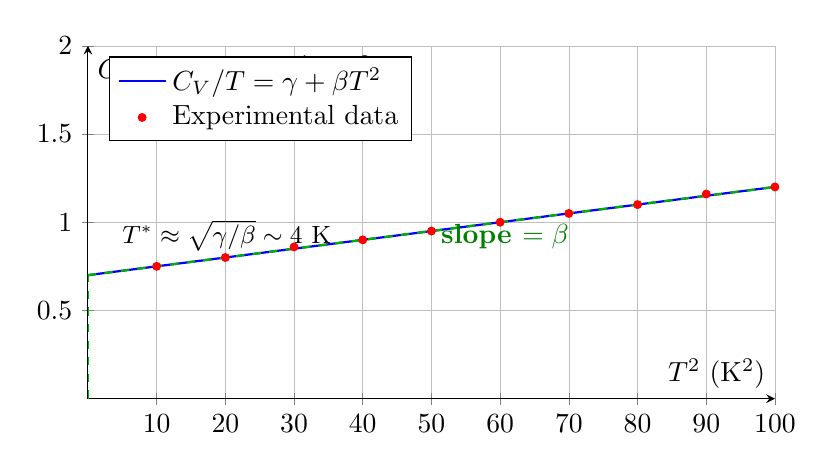
\begin{tikzpicture}
\begin{axis}[
    width=0.85\textwidth,
    height=0.5\textwidth,
    xlabel={$T^2$ (K$^2$)},
    ylabel={$C_V/T$ (mJ mol$^{-1}$ K$^{-2}$)},
    xmin=0, xmax=100,
    ymin=0, ymax=2.0,
    legend pos=north west,
    legend cell align=left,
    grid=both,
    grid style={line width=.1pt, draw=gray!20},
    major grid style={line width=.2pt,draw=gray!50},
    axis lines=middle,
    samples=200,
]
% Linear fit C/T = gamma + beta T^2
\addplot[blue, thick, domain=0:100] {0.7 + 0.005*x};
\addlegendentry{$C_V/T = \gamma + \beta T^2$}

% Data points (simulated, with small noise)
\addplot[only marks, mark=*, mark size=1.4pt, red] coordinates {
    (10, 0.75) (20, 0.80) (30, 0.86) (40, 0.90) (50, 0.95) (60, 1.00) (70, 1.05) (80, 1.10) (90, 1.16) (100, 1.20)
};
\addlegendentry{Experimental data}

% Intercept gamma
\addplot[green!70!black, dashed, thick] coordinates {(0, 0) (0, 0.7)};
\node[anchor=east, green!50!black, font=\bfseries] at (axis cs:0, 0.7) {$\gamma$};

% Slope annotation: dashed line from intercept
\addplot[green!70!black, dashed, thick] coordinates {(0, 0.7) (100, 1.2)};
\node[anchor=west, green!50!black, font=\bfseries] at (axis cs:50, 0.92) {slope $=\beta$};

% Crossover T*
\node[anchor=south west, font=\small, black] at (axis cs:3.6, 0.78) {$T^*\approx\sqrt{\gamma/\beta}\sim 4$ K};
\end{axis}
\end{tikzpicture}
\caption{Plot of $C_V/T$ versus $T^2$ for a metal such as copper. The intercept gives the Sommerfeld coefficient $\gamma$ (electronic contribution), and the slope gives $\beta$ (phonon contribution). Below the crossover temperature $T^*=\sqrt{\gamma/\beta}$, the linear electronic term dominates.}
\label{fig:specific_heat}
\end{figure}

\begin{methodbox}{Extracting $\gamma$ and $\Theta_D$ from Calorimetric Data}
To extract physical parameters from experimental low-temperature specific heat data:
\begin{enumerate}
    \item Tabulate experimental $(T_i, C_i)$ points in the range $1\ \mathrm{K} \le T \le 4\ \mathrm{K}$.
    \item Construct a linear regression of $Y = C/T$ against $X = T^2$.
    \item Identify the intercept $Y_0 = \gamma$ in $\mathrm{mJ\,mol^{-1}\,K^{-2}}$.
    \item Extract the Fermi energy via $E_F = \frac{\pi^2 R k_B}{2\gamma}$.
    \item Identify the slope $m = \beta$ in $\mathrm{mJ\,mol^{-1}\,K^{-4}}$, and calculate the Debye temperature:
    \[
    \Theta_D = \left( \frac{12\pi^4 R}{5\beta} \right)^{1/3}
    \]
\end{enumerate}
\end{methodbox}

\subsection{Pauli Spin Paramagnetism of the Free Electron Gas}
In classical statistical mechanics, magnetic moments of magnitude $\mu_B$ in an applied magnetic field $B$ align according to the Langevin--Curie law:
\begin{equation}
\chi_{\mathrm{Curie}} = \frac{\mu_0 n \mu_B^2}{k_B T} \propto \frac{1}{T}
\end{equation}
However, non-ferromagnetic metals (such as Na, Al, Cu) display an extremely weak, nearly \textbf{temperature-independent paramagnetism}. Wolfgang Pauli (1927) explained this phenomenon as another fundamental consequence of Fermi--Dirac quantum statistics.

Each electron possesses an intrinsic magnetic dipole moment $\bm{\mu}_s = -g \mu_B \vb{S}/\hbar = \mp \mu_B$ directed antiparallel to its spin. In an external magnetic field $\vb{B} = B\hat{z}$, the Zeeman interaction energy is:
\begin{equation}
\Delta E = -\bm{\mu}_s \cdot \vb{B} = \pm \mu_B B
\end{equation}
\begin{itemize}
    \item Electrons with spin parallel to $\vb{B}$ (magnetic moment parallel, spin $\downarrow$) have their energy lowered: $E_\downarrow = E - \mu_B B$.
    \item Electrons with spin antiparallel to $\vb{B}$ (magnetic moment antiparallel, spin $\uparrow$) have their energy raised: $E_\uparrow = E + \mu_B B$.
\end{itemize}

\begin{figure}[h]
\centering
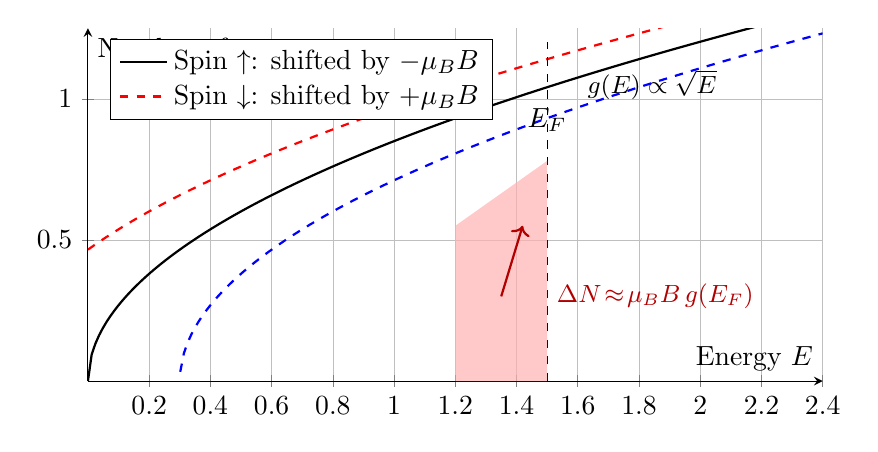
\begin{tikzpicture}
\begin{axis}[
    width=0.9\textwidth,
    height=0.5\textwidth,
    xlabel={Energy $E$},
    ylabel={Number of states},
    xmin=0, xmax=2.4,
    ymin=0, ymax=1.25,
    legend pos=north west,
    legend cell align=left,
    grid=both,
    grid style={line width=.1pt, draw=gray!20},
    major grid style={line width=.2pt,draw=gray!50},
    axis lines=middle,
    samples=200,
]
% DOS sqrt(E) - 3D
\addplot[black, thick, domain=0:2.4] {0.85*sqrt(x)};
\node[anchor=west, font=\small] at (axis cs:1.6, 1.05) {$g(E)\propto\sqrt{E}$};

% Spin-up shifted down (B>0 favors spin up)
\addplot[red, thick, dashed, domain=0:2.4] {0.85*sqrt(x+0.3)};
\addlegendentry{Spin $\uparrow$: shifted by $-\mu_B B$}

% Spin-down shifted up
\addplot[blue, thick, dashed, domain=0:2.4] {0.85*sqrt(x-0.3)};
\addlegendentry{Spin $\downarrow$: shifted by $+\mu_B B$}

% Fermi level
\addplot[black, dashed] coordinates {(1.5,0) (1.5,1.2)};
\node[anchor=south, font=\bfseries] at (axis cs:1.5, 0.85) {$E_F$};

% Imbalance shading
\fill[red!30, opacity=0.7] (axis cs:1.2, 0) -- (axis cs:1.5, 0) -- (axis cs:1.5, 0.78) -- (axis cs:1.2, 0.55) -- cycle;
\draw[->, thick, red!70!black] (axis cs:1.35, 0.30) -- (axis cs:1.42, 0.55);
\node[anchor=west, font=\small, red!70!black] at (axis cs:1.5, 0.30) {$\Delta N\!\approx\!\mu_B B\,g(E_F)$};
\end{axis}
\end{tikzpicture}
\caption{Pauli paramagnetism: in a magnetic field $B$, spin-up and spin-down DOS curves shift in opposite directions by $\pm\mu_B B$. Electrons near $E_F$ flip to the lower-energy (spin-up) state, producing a net magnetization $M=\mu_B^2 B\,g(E_F)$. Only states within $\sim\mu_B B$ of $E_F$ contribute, so $\chi\propto g(E_F)$ is essentially $T$-independent.}
\label{fig:pauli}
\end{figure}

Because electrons can flip their spin via spin-orbit interactions to reach thermal equilibrium, electrons near the Fermi boundary transfer from the higher-energy sub-band to the lower-energy sub-band until both spin manifolds share a common chemical potential $\mu$.

The energy shift between the two sub-bands is $2\mu_B B$. The number of electrons transferred from spin-up to spin-down is the density of states per spin channel ($\frac{1}{2}g(E_F)$) multiplied by the Zeeman energy shift $\mu_B B$:
\begin{equation}
\Delta N = N_\downarrow - N_\uparrow \approx 2 \times \left[ \frac{1}{2}g(E_F) \mu_B B \right] = g(E_F) \mu_B B
\end{equation}
The resulting net macroscopic magnetization $M$ is:
\begin{equation}
M = \mu_B \Delta N = \mu_B^2 g(E_F) B
\end{equation}
The \textbf{Pauli paramagnetic volume susceptibility} $\chi_{\mathrm{Pauli}} \equiv \mu_0 M/B$ is:
\begin{equation}
\boxed{\chi_{\mathrm{Pauli}} = \mu_0 \mu_B^2 g(E_F) = \frac{3\mu_0 n \mu_B^2}{2E_F}}
\label{eq:pauli_susceptibility}
\end{equation}
Notice that $\chi_{\mathrm{Pauli}}$ depends strictly on the density of states at the Fermi level $g(E_F)$ and is \textbf{completely independent of temperature} to leading order! Thermal corrections enter only at order $(T/T_F)^2 \sim 10^{-4}$, perfectly explaining the experimental observations.

\vspace{0.4cm}

% -------------------------------------------------------------------------
% SOLVED EXAMPLES FOR CHAPTER 4
% -------------------------------------------------------------------------
\begin{examplebox}{Energy Levels for Given Fermi--Dirac Probabilities}{ex:fd_probabilities}
\textbf{Problem Statement:}
For metallic sodium at room temperature ($T = 300\ \mathrm{K}$, $k_B T \approx 0.02585\ \mathrm{eV}$), the chemical potential is $\mu = 3.130\ \mathrm{eV}$. Find the energy levels $E$ for which the Fermi--Dirac occupation probability is:
(a) $f(E) = 0.50$, (b) $f(E) = 0.75$, and (c) $f(E) = 0.25$.

\vspace{0.2cm}\hrule\vspace{0.2cm}
\textbf{Step-by-Step Solution:}

Inverting the Fermi--Dirac distribution function $f(E) = \frac{1}{e^{(E-\mu)/k_BT} + 1}$:
\[
e^{(E-\mu)/k_BT} + 1 = \frac{1}{f} \implies e^{(E-\mu)/k_BT} = \frac{1-f}{f} \implies E = \mu + k_B T \ln\left(\frac{1-f}{f}\right)
\]

\textbf{(a) Case $f = 0.50$:}
\[
\frac{1-0.50}{0.50} = 1 \implies \ln(1) = 0 \implies E = \mu = \mathbf{3.130\ \mathrm{eV}}
\]

\textbf{(b) Case $f = 0.75$:}
\[
\frac{1-0.75}{0.75} = \frac{0.25}{0.75} = \frac{1}{3}
\]
\[
E = \mu + k_B T \ln(1/3) = \mu - k_B T \ln(3) = 3.130\ \mathrm{eV} - (0.02585\ \mathrm{eV})(1.0986) = 3.130 - 0.0284 \approx \mathbf{3.102\ \mathrm{eV}}
\]

\textbf{(c) Case $f = 0.25$:}
\[
\frac{1-0.25}{0.25} = \frac{0.75}{0.25} = 3
\]
\[
E = \mu + k_B T \ln(3) = 3.130\ \mathrm{eV} + 0.0284\ \mathrm{eV} \approx \mathbf{3.158\ \mathrm{eV}}
\]
\textbf{Physical Insight:} Notice that the energy shifts are perfectly symmetric: $E(0.75) = \mu - 1.10 k_B T$ and $E(0.25) = \mu + 1.10 k_B T$, illustrating exact particle-hole symmetry around the chemical potential.
\end{examplebox}

\vspace{0.4cm}

\begin{examplebox}{Proof of Particle-Hole Symmetry of the Fermi Function}{ex:particle_hole_proof}
\textbf{Problem Statement:}
Prove analytically that the Fermi--Dirac distribution function satisfies the exact particle-hole identity:
\[
f(\mu + \Delta) + f(\mu - \Delta) \equiv 1 \quad \text{for all } \Delta \text{ and all } T > 0
\]

\vspace{0.2cm}\hrule\vspace{0.2cm}
\textbf{Step-by-Step Proof:}

Let $x \equiv \Delta / (k_B T)$. Then:
\[
f(\mu + \Delta) = \frac{1}{e^x + 1}, \quad f(\mu - \Delta) = \frac{1}{e^{-x} + 1}
\]
Multiply the numerator and denominator of $f(\mu - \Delta)$ by $e^x$:
\[
f(\mu - \Delta) = \frac{1 \cdot e^x}{(e^{-x} + 1)e^x} = \frac{e^x}{1 + e^x}
\]
Adding the two terms:
\[
f(\mu + \Delta) + f(\mu - \Delta) = \frac{1}{e^x + 1} + \frac{e^x}{e^x + 1} = \frac{1 + e^x}{e^x + 1} \equiv \mathbf{1} \quad \text{\textbf{Q.E.D.}}
\]
\end{examplebox}

\vspace{0.4cm}

\begin{examplebox}{Sommerfeld Heat Capacity Coefficient of Aluminum}{ex:al_gamma}
\textbf{Problem Statement:}
Metallic aluminum has a Fermi energy $E_F = 11.7\ \mathrm{eV}$ and valence $Z_v = 3$. Calculate the theoretical molar Sommerfeld coefficient $\gamma$ in $\mathrm{mJ\,mol^{-1}\,K^{-2}}$, and determine the electronic heat capacity at $T = 4.2\ \mathrm{K}$.

\vspace{0.2cm}\hrule\vspace{0.2cm}
\textbf{Step-by-Step Solution:}

\textbf{(a) Molar Sommerfeld coefficient $\gamma$:}
First convert $E_F$ to Joules:
\[
E_F = (11.7\ \mathrm{eV})(1.6022 \times 10^{-19}\ \mathrm{J/eV}) \approx 1.875 \times 10^{-18}\ \mathrm{J}
\]
For one mole of aluminum ($N_A$ atoms), each atom contributes $3$ conduction electrons, so $N = 3 N_A$. The electronic heat capacity coefficient is:
\[
\gamma = \frac{\pi^2}{2}\frac{N k_B^2}{E_F} = \frac{\pi^2}{2}\frac{(3 N_A) k_B^2}{E_F} = \frac{3\pi^2 R k_B}{2 E_F}
\]
Evaluating with $R = 8.3145\ \mathrm{J/(mol\cdot K)}$:
\begin{align*}
\gamma &= \frac{3\pi^2 (8.3145\ \mathrm{J/(mol\cdot K)})(1.3807 \times 10^{-23}\ \mathrm{J/K})}{2(1.875 \times 10^{-18}\ \mathrm{J})} \\
&= \frac{3.400 \times 10^{-21}}{3.750 \times 10^{-18}} \approx 9.07 \times 10^{-4}\ \mathrm{J\,mol^{-1}\,K^{-2}} = \mathbf{0.907\ \mathrm{mJ\,mol^{-1}\,K^{-2}}}
\end{align*}
(If calculated per mole of electrons, $\gamma_e = \frac{\pi^2 R k_B}{2E_F} \approx 0.302\ \mathrm{mJ\,mol^{-1}\,K^{-2}}$).

\textbf{(b) Electronic heat capacity at $T = 4.2\ \mathrm{K}$:}
\[
C_{el}(4.2\ \mathrm{K}) = \gamma T = (0.907\ \mathrm{mJ\,mol^{-1}\,K^{-2}})(4.2\ \mathrm{K}) \approx \mathbf{3.81\ \mathrm{mJ\,mol^{-1}\,K^{-1}}}
\]
\end{examplebox}

\vspace{0.4cm}

\begin{examplebox}{Electronic vs. Lattice Specific Heat Crossover in Copper}{ex:copper_crossover}
\textbf{Problem Statement:}
Low-temperature calorimetric measurements on copper yield a molar Sommerfeld coefficient $\gamma = 0.695\ \mathrm{mJ\,mol^{-1}\,K^{-2}}$ and a Debye phonon coefficient $\beta = 0.048\ \mathrm{mJ\,mol^{-1}\,K^{-4}}$.
\begin{enumerate}[label=(\alph*)]
    \item Determine the Debye characteristic temperature $\Theta_D$ of copper.
    \item Calculate the crossover temperature $T^*$ where electronic and lattice heat capacities are equal.
    \item Compare the electronic and lattice contributions at $T = 1.0\ \mathrm{K}$ and at $T = 300\ \mathrm{K}$.
\end{enumerate}

\vspace{0.2cm}\hrule\vspace{0.2cm}
\textbf{Step-by-Step Solution:}

\textbf{(a) Debye temperature $\Theta_D$:}
Using equation~\eqref{eq:debye_beta} with $\beta = 0.048 \times 10^{-3}\ \mathrm{J\,mol^{-1}\,K^{-4}}$:
\begin{align*}
\Theta_D &= \left( \frac{12\pi^4 R}{5\beta} \right)^{1/3} = \left( \frac{12\pi^4 (8.3145)}{5(4.8 \times 10^{-5})} \right)^{1/3} = \left( \frac{9719}{2.4 \times 10^{-4}} \right)^{1/3} = (4.05 \times 10^7)^{1/3} \approx \mathbf{343.4\ \mathrm{K}}
\end{align*}

\textbf{(b) Crossover temperature $T^*$:}
Setting $C_{el} = C_{ph} \implies \gamma T^* = \beta (T^*)^3$:
\[
T^* = \sqrt{\frac{\gamma}{\beta}} = \sqrt{\frac{0.695\ \mathrm{mJ\,mol^{-1}\,K^{-2}}}{0.048\ \mathrm{mJ\,mol^{-1}\,K^{-4}}}} = \sqrt{14.48} \approx \mathbf{3.81\ \mathrm{K}}
\]

\textbf{(c) Contribution comparison:}
\begin{itemize}
    \item At $T = 1.0\ \mathrm{K}$:
    \[
    C_{el} = (0.695)(1.0) = 0.695\ \mathrm{mJ/mol\cdot K}, \quad C_{ph} = (0.048)(1.0)^3 = 0.048\ \mathrm{mJ/mol\cdot K}
    \]
    The electronic heat capacity is $\mathbf{14.5\ \text{times larger}}$ than the phonon contribution!
    \item At $T = 300\ \mathrm{K}$ (room temperature):
    \[
    C_{el} = (0.695 \times 10^{-3}\ \mathrm{J/mol\cdot K^2})(300\ \mathrm{K}) \approx \mathbf{0.208\ \mathrm{J/(mol\cdot K)}}
    \]
    The high-temperature Dulong--Petit phonon heat capacity is $C_{ph} \approx 3R \approx \mathbf{24.94\ \mathrm{J/(mol\cdot K)}}$.
    The electronic fraction at room temperature is only:
    \[
    \frac{C_{el}}{C_{\mathrm{total}}} \approx \frac{0.208}{25.15} \approx \mathbf{0.83\%}
    \]
\end{itemize}
\end{examplebox}

\clearpage


% =========================================================================
% CHAPTER 5: ELECTRICAL & THERMAL TRANSPORT IN METALS
% =========================================================================
\section{Electrical and Thermal Transport in Metals}
\label{sec:transport_phenomena}

\subsection{Semiclassical Dynamics of Conduction Electrons}
In the quantum Sommerfeld model, conduction electrons are treated as localized wavepackets formed by a coherent superposition of plane waves centered at wavevector $\vb{k}$. The center-of-mass dynamics of an electron wavepacket in external macroscopic electromagnetic fields obeys the \textbf{semiclassical equations of motion}:
\begin{align}
\vb{v}(\vb{k}) &= \frac{1}{\hbar}\nabla_{\vb{k}} E(\vb{k}) \label{eq:group_velocity} \\
\hbar \frac{d\vb{k}}{dt} &= \vb{F}_{\mathrm{ext}} = -e\left( \vb{E} + \vb{v}\times\vb{B} \right) \label{eq:semiclassical_acceleration}
\end{align}
where $\vb{v}(\vb{k})$ is the quantum group velocity. For a parabolic, isotropic free-electron dispersion $E(\vb{k}) = \frac{\hbar^2 k^2}{2m_e}$, the group velocity simplifies directly to the classical momentum relation:
\begin{equation}
\vb{v}(\vb{k}) = \frac{1}{\hbar}\nabla_{\vb{k}}\left(\frac{\hbar^2 k^2}{2m_e}\right) = \frac{\hbar \vb{k}}{m_e}
\end{equation}

\subsection{The Boltzmann Transport Equation in the Relaxation Time Approximation}
To describe transport in non-equilibrium conditions, we define the distribution function $f(\vb{r}, \vb{k}, t)$ such that:
\begin{equation}
dn = 2 \times f(\vb{r}, \vb{k}, t) \frac{d^3r\, d^3k}{(2\pi)^3}
\end{equation}
represents the number of electrons in the six-dimensional phase-space volume element $d^3r\, d^3k$ at time $t$ (the factor of 2 accounts for spin).

According to Liouville's theorem, in the presence of external forces and microscopic scattering collisions, the total time rate of change of $f$ is:
\begin{equation}
\frac{df}{dt} = \frac{\partial f}{\partial t} + \vb{v}\cdot\nabla_{\vb{r}}f + \dot{\vb{k}}\cdot\nabla_{\vb{k}}f = \left(\frac{\partial f}{\partial t}\right)_{\mathrm{coll}}
\label{eq:bte_full}
\end{equation}
Under the \textbf{Relaxation Time Approximation} (RTA), the collision integral is modeled as an exponential decay toward the local Fermi--Dirac equilibrium distribution $f_0$:
\begin{equation}
\left(\frac{\partial f}{\partial t}\right)_{\mathrm{coll}} = -\frac{f(\vb{r}, \vb{k}, t) - f_0(E)}{\tau(\vb{k})}
\label{eq:bte_rta}
\end{equation}
where $\tau(\vb{k})$ is the momentum relaxation time. 

For steady-state ($\partial f/\partial t = 0$), spatially homogeneous ($\nabla_{\vb{r}}f = 0$) conduction driven by a uniform electric field $\vb{E}$, the wavevector acceleration is $\dot{\vb{k}} = -e\vb{E}/\hbar$. The Boltzmann equation~\eqref{eq:bte_full} reduces to:
\begin{equation}
-\frac{e\vb{E}}{\hbar}\cdot\nabla_{\vb{k}}f = -\frac{f - f_0}{\tau}
\label{eq:bte_steady}
\end{equation}

\subsection{Linearization of the Distribution Function}
For ordinary electric fields ($E \sim 1\text{--}100\ \mathrm{V/m}$), the perturbation away from equilibrium is exceedingly small. We linearize the distribution function:
\begin{equation}
f(\vb{k}) \approx f_0(E(\vb{k})) + f_1(\vb{k}), \quad |f_1| \ll f_0
\label{eq:f_linearization}
\end{equation}
Substituting equation~\eqref{eq:f_linearization} into the left-hand side of equation~\eqref{eq:bte_steady} and approximating $\nabla_{\vb{k}}f \approx \nabla_{\vb{k}}f_0$:
\begin{equation}
\nabla_{\vb{k}}f_0 = \frac{\partial f_0}{\partial E}\nabla_{\vb{k}}E = \hbar\vb{v}\frac{\partial f_0}{\partial E}
\end{equation}
Equation~\eqref{eq:bte_steady} becomes:
\begin{equation}
-\frac{e\vb{E}}{\hbar}\cdot\left(\hbar\vb{v}\frac{\partial f_0}{\partial E}\right) = -\frac{f_1}{\tau}
\end{equation}
Solving directly for the non-equilibrium perturbation $f_1(\vb{k})$:
\begin{equation}
\boxed{f_1(\vb{k}) = e\tau(\vb{v}\cdot\vb{E})\left(-\frac{\partial f_0}{\partial E}\right)}
\label{eq:f1_solution}
\end{equation}
\paragraph{Physical Interpretation (Shifted Fermi Sphere):}
Notice that for an electric field along $+x$, $\vb{v}\cdot\vb{E} = v_x E_x$. Since $\vb{v} = \frac{\hbar\vb{k}}{m_e}$:
\begin{equation}
f(\vb{k}) \approx f_0(E) + \frac{e\tau E_x}{\hbar}\frac{\partial E}{\partial k_x}\left(-\frac{\partial f_0}{\partial E}\right) = f_0(E) - \Delta k_x \frac{\partial f_0}{\partial k_x} \approx f_0\left(k_x + \frac{e E_x \tau}{\hbar}, k_y, k_z\right)
\end{equation}
The application of an electric field simply shifts the entire Fermi sphere in reciprocal space rigidly opposite to the electric field by a displacement:
\begin{equation}
\boxed{\Delta\vb{k} = -\frac{e\vb{E}\tau}{\hbar}}
\label{eq:k_shift}
\end{equation}

\subsection{Rigorous Evaluation of Current Density and Conductivity Recovery}
The macroscopic electric current density is obtained by integrating the velocity of all occupied states over $k$-space:
\begin{equation}
\vb{j} = -2e\int \frac{d^3k}{(2\pi)^3}\vb{v}(\vb{k}) f(\vb{k}) = -2e\int \frac{d^3k}{(2\pi)^3}\vb{v}(\vb{k})\left[ f_0(E) + f_1(\vb{k}) \right]
\label{eq:j_integral_split}
\end{equation}
The integral splits naturally into two parts:
\begin{enumerate}
    \item \textbf{Equilibrium Integral} ($I_0$):
    \begin{equation}
    \vb{j}_0 = -2e\int \frac{d^3k}{(2\pi)^3}\vb{v}(\vb{k})f_0(E(\vb{k})) = \vb{0}
    \end{equation}
    The equilibrium current vanishes identically because $E(\vb{k})$ and $f_0(E(\vb{k}))$ are even functions of $\vb{k}$ ($f_0(-\vb{k}) = f_0(\vb{k})$), whereas velocity $\vb{v}(\vb{k}) = \hbar\vb{k}/m_e$ is strictly odd ($\vb{v}(-\vb{k}) = -\vb{v}(\vb{k})$).
    \item \textbf{Transport Integral} ($I_1$):
    For an electric field applied along $\hat{x}$ ($\vb{E} = E_x\hat{x}$):
    \begin{equation}
    j_x = -2e\int \frac{d^3k}{(2\pi)^3}v_x(\vb{k})\left[ e\tau v_x E_x \left(-\frac{\partial f_0}{\partial E}\right) \right] = \frac{e^2\tau E_x}{4\pi^3}\int d^3k\, v_x^2 \left(-\frac{\partial f_0}{\partial E}\right)
    \label{eq:jx_transport_integral}
    \end{equation}
\end{enumerate}

\paragraph{Coordinate Transformation to Iso-Energetic Surfaces:}
We transform the 3D volume element $d^3k$ into an integral over constant-energy surfaces $S_E$ in $k$-space:
\begin{equation}
d^3k = dS_E dk_\perp = dS_E \frac{dE}{|\nabla_{\vb{k}}E|} = \frac{dS_E dE}{\hbar v}
\label{eq:iso_energetic_coords}
\end{equation}
For an isotropic, spherical Fermi surface, directional averaging gives $\langle v_x^2 \rangle = \frac{1}{3}v^2$. Thus:
\begin{equation}
v_x^2 d^3k = \left(\frac{1}{3}v^2\right) \frac{dS_E dE}{\hbar v} = \frac{1}{3\hbar} v(E) dS_E dE
\end{equation}
Substituting into equation~\eqref{eq:jx_transport_integral}:
\begin{equation}
j_x = \frac{e^2\tau E_x}{12\pi^3\hbar}\int_0^\infty dE\left(-\frac{\partial f_0}{\partial E}\right) v(E)\iint_{S_E} dS_E
\end{equation}
For a sphere in $k$-space, $\iint_{S_E} dS_E = 4\pi k^2$. 

At low temperatures ($T \ll T_F$), the derivative $-\frac{\partial f_0}{\partial E}$ collapses to a Dirac delta function centered at the Fermi energy:
\begin{equation}
\lim_{T\to 0}\left(-\frac{\partial f_0}{\partial E}\right) = \delta(E - E_F)
\end{equation}
The energy integral collapses instantly to the Fermi surface:
\begin{equation}
j_x = \frac{e^2\tau E_x}{12\pi^3\hbar} v_F (4\pi k_F^2) = \frac{e^2\tau E_x}{3\pi^2\hbar} v_F k_F^2
\end{equation}
Using $v_F = \frac{\hbar k_F}{m_e}$:
\begin{equation}
j_x = \frac{e^2\tau E_x}{3\pi^2\hbar}\left(\frac{\hbar k_F}{m_e}\right)k_F^2 = \left( \frac{e^2\tau k_F^3}{3\pi^2 m_e} \right)E_x
\end{equation}
Recalling the fundamental relation from Chapter~2, $k_F^3 = 3\pi^2 n$:
\begin{equation}
\boxed{j_x = \left(\frac{n e^2 \tau}{m_e}\right)E_x \implies \sigma = \frac{n e^2 \tau}{m_e}}
\label{eq:quantum_sigma_recovery}
\end{equation}
We have rigorously recovered Drude's classical conductivity formula from first-principles quantum Boltzmann transport theory!

\begin{checkpointbox}{Why Electrical Conduction Occurs Exclusively at the Fermi Surface}
The appearance of the Dirac delta function $\delta(E - E_F)$ proves mathematically that \textbf{electrons deep inside the Fermi sea carry zero net current}! 

Under an electric field, for every state $(k_x, k_y, k_z)$ filled deep below $E_F$, the time-reversed state $(-k_x, k_y, k_z)$ is also completely filled. Their equal and opposite velocities cancel out identically. Only right at the Fermi sphere boundary does the field populate forward states while depopulating backward states, creating an uncompensated current carrying surface layer.
\end{checkpointbox}

\subsection{Microscopic Scattering Mechanisms and Matthiessen's Rule}
In a pure metal, the carrier density $n$ is temperature-independent. The observed temperature dependence of electrical resistivity $\rho(T) = \frac{m_e}{n e^2 \tau(T)}$ is governed entirely by the microscopic collision time $\tau(T)$.

Electrons in a crystal experience two independent scattering processes:
\begin{enumerate}[leftmargin=*]
    \item \textbf{Impurity and Defect Scattering}: Electrons scatter elastically from stationary disruptions of lattice periodicity (chemical impurities, vacancies, interstitials, and grain boundaries). Because static defects do not freeze out at low temperatures, the impurity collision time $\tau_{\mathrm{imp}}$ is independent of temperature, giving rise to a constant \textbf{residual resistivity} $\rho_0$:
    \begin{equation}
    \rho_0 = \frac{m_e}{n e^2 \tau_{\mathrm{imp}}}
    \end{equation}
    \item \textbf{Thermal Phonon Scattering}: Electrons scatter inelastically from quantized lattice vibrations (phonons). At temperatures well above the Debye temperature ($T > \Theta_D$), the thermal phonon population is proportional to temperature ($n_{\mathrm{ph}} \propto T$), leading to a scattering rate $\tau_{\mathrm{ph}}^{-1} \propto T$ and a lattice resistivity $\rho_{\mathrm{ph}}(T) \propto T$. At low temperatures ($T \ll \Theta_D$), small-angle scattering leads to the Bloch $T^5$ law ($\rho_{\mathrm{ph}} \propto T^5$).
\end{enumerate}
Because impurity and phonon scattering events are statistically independent, their scattering probabilities per unit time add linearly:
\begin{equation}
\boxed{\frac{1}{\tau(T)} = \frac{1}{\tau_{\mathrm{imp}}} + \frac{1}{\tau_{\mathrm{ph}}(T)}}
\label{eq:scattering_rates_sum}
\end{equation}
Multiplying by $\frac{m_e}{ne^2}$ yields \textbf{Matthiessen's Rule}:
\begin{equation}
\boxed{\rho(T) = \rho_0 + \rho_{\mathrm{ph}}(T)}
\label{eq:matthiessens_rule}
\end{equation}
Matthiessen's rule is widely utilized to quantify crystal purity via the \textbf{Residual Resistivity Ratio} ($\mathrm{RRR} \equiv \rho(300\ \mathrm{K})/\rho(4.2\ \mathrm{K})$), and forms the physical operating principle of ultra-stable \textbf{Platinum Resistance Thermometers} (PRTs).

\subsection{Quantum Thermal Conductivity and the Wiedemann--Franz Law}
In metals, thermal energy is conducted predominantly by the mobile conduction electrons; the lattice phonon contribution to thermal conductivity is negligible by comparison ($K_{el} \gg K_{ph}$).

From kinetic gas theory, the thermal conductivity $K$ of a gas of particles moving with characteristic speed $v$ and mean free path $l = v\tau$ is:
\begin{equation}
K = \frac{1}{3} C_V v l = \frac{1}{3} C_{el} v_F^2 \tau
\label{eq:kinetic_quantum_k}
\end{equation}
In the quantum Sommerfeld model, the carriers that transport thermal energy are the electrons near the Fermi boundary, which move at the Fermi velocity $v = v_F$.

Substituting the exact quantum electronic specific heat per unit volume $C_{el} = \frac{\pi^2}{2} n k_B \left(\frac{T}{T_F}\right) = \frac{\pi^2 n k_B^2 T}{m_e v_F^2}$ into equation~\eqref{eq:kinetic_quantum_k}:
\begin{equation}
K_{el} = \frac{1}{3}\left( \frac{\pi^2 n k_B^2 T}{m_e v_F^2} \right) v_F (v_F \tau) = \frac{\pi^2 n k_B^2 \tau T}{3m_e}
\label{eq:quantum_thermal_conductivity}
\end{equation}
Now, take the ratio of the electronic thermal conductivity $K_{el}$ to the electrical conductivity $\sigma = \frac{ne^2\tau}{m_e}$:
\begin{equation}
\frac{K_{el}}{\sigma} = \frac{\frac{\pi^2 n k_B^2 \tau T}{3m_e}}{\frac{n e^2\tau}{m_e}} = \frac{\pi^2 k_B^2}{3 e^2} T
\end{equation}
Dividing by absolute temperature $T$ yields the universal \textbf{Wiedemann--Franz Law}:
\begin{equation}
\boxed{\frac{K}{\sigma T} = \frac{\pi^2}{3}\left(\frac{k_B}{e}\right)^2 \equiv L}
\label{eq:quantum_wf_law}
\end{equation}
The theoretical \textbf{Sommerfeld Lorenz number} is:
\begin{equation}
L = \frac{\pi^2}{3}\left(\frac{1.3807 \times 10^{-23}\ \mathrm{J/K}}{1.6022 \times 10^{-19}\ \mathrm{C}}\right)^2 = \mathbf{2.443 \times 10^{-8}\ \mathrm{W\,\Omega\,K^{-2}}}
\label{eq:sommerfeld_lorenz_val}
\end{equation}

\begin{takeawaybox}{The Universality of the Lorenz Number}
The Sommerfeld Lorenz number $L = \frac{\pi^2}{3}(k_B/e)^2$ is a fundamental constant of nature. It contains:
\begin{itemize}
    \item NO dependence on electron density $n$.
    \item NO dependence on electron effective mass $m_e$.
    \item NO dependence on the microscopic scattering relaxation time $\tau$.
\end{itemize}
This explains why metals as diverse as copper, silver, gold, platinum, and lead all exhibit virtually identical Lorenz numbers at room temperature!
\end{takeawaybox}

\begin{table}[ht]
\centering
\small
\renewcommand{\arraystretch}{1.25}
\begin{tabular}{lcc}
\toprule
\textbf{Metal} & \textbf{Lorenz Number at $0^\circ\mathrm{C}$} ($10^{-8}\ \mathrm{W\,\Omega\,K^{-2}}$) & \textbf{Lorenz Number at $100^\circ\mathrm{C}$} ($10^{-8}\ \mathrm{W\,\Omega\,K^{-2}}$) \\
\midrule
\textbf{Silver (Ag)}    & 2.31 & 2.37 \\
\textbf{Copper (Cu)}    & 2.23 & 2.33 \\
\textbf{Gold (Au)}      & 2.35 & 2.40 \\
\textbf{Platinum (Pt)}  & 2.51 & 2.60 \\
\textbf{Lead (Pb)}      & 2.47 & 2.56 \\
\textbf{Aluminum (Al)}  & 2.14 & 2.19 \\
\midrule
\textbf{Theoretical Value} & \multicolumn{2}{c}{$\mathbf{2.443 \times 10^{-8}\ \mathrm{W\,\Omega\,K^{-2}}}$} \\
\bottomrule
\end{tabular}
\caption{Comparison of experimental Lorenz numbers for representative metals with the Sommerfeld quantum prediction.}
\label{tab:lorenz_table}
\end{table}

\vspace{0.4cm}

% -------------------------------------------------------------------------
% SOLVED EXAMPLES FOR CHAPTER 5
% -------------------------------------------------------------------------
\begin{examplebox}{Derivation of Electrical Conductivity from the Boltzmann Equation}{ex:bte_conductivity_derivation}
\textbf{Problem Statement:}
Starting from the steady-state Boltzmann Transport Equation $-\frac{e\vb{E}}{\hbar}\cdot\nabla_{\vb{k}}f = -\frac{f - f_0}{\tau}$, provide a complete mathematical derivation showing that the DC conductivity for an isotropic 3D parabolic band is $\sigma = \frac{n e^2 \tau}{m_e}$.

\vspace{0.2cm}\hrule\vspace{0.2cm}
\textbf{Step-by-Step Derivation:}

\textbf{1. Linearization:}
Let $f(\vb{k}) = f_0(E) + f_1(\vb{k})$. Since $f_0$ depends on $\vb{k}$ through energy $E(\vb{k})$:
\[
\nabla_{\vb{k}}f_0 = \frac{\partial f_0}{\partial E}\nabla_{\vb{k}}E = \hbar\vb{v}\frac{\partial f_0}{\partial E}
\]
Substituting into the BTE gives:
\[
-\frac{e\vb{E}}{\hbar}\cdot\left(\hbar\vb{v}\frac{\partial f_0}{\partial E}\right) = -\frac{f_1}{\tau} \implies f_1 = e\tau(\vb{v}\cdot\vb{E})\left(-\frac{\partial f_0}{\partial E}\right)
\]

\textbf{2. Current Density Integral:}
Choosing $\vb{E} = E_x\hat{x}$, the current density along $x$ is:
\[
j_x = -2e\int \frac{d^3k}{(2\pi)^3} v_x [f_0(E) + f_1(\vb{k})] = -2e\int \frac{d^3k}{(2\pi)^3} v_x f_0(E) + 2e^2\tau E_x \int \frac{d^3k}{(2\pi)^3} v_x^2 \left(-\frac{\partial f_0}{\partial E}\right)
\]
The first integral vanishes because $v_x = \hbar k_x/m$ is odd in $k_x$ while $f_0(E(k))$ is even.

\textbf{3. Surface Integration:}
Transforming to spherical $k$-space coordinates: $d^3k = k^2 dk\, d\Omega = k^2 dk \sin\theta d\theta d\phi$. In spherical symmetry, $\langle v_x^2 \rangle = \frac{1}{3}v^2$:
\[
j_x = \frac{2e^2\tau E_x}{(2\pi)^3} \int_0^\infty k^2 dk \left( \frac{1}{3}v(k)^2 \right)\left(-\frac{\partial f_0}{\partial E}\right) \int d\Omega = \frac{2e^2\tau E_x}{8\pi^3}(4\pi) \int_0^\infty \frac{1}{3} v(k)^2 k^2 dk \left(-\frac{\partial f_0}{\partial E}\right)
\]
Using $E = \frac{\hbar^2 k^2}{2m} \implies dE = \frac{\hbar^2 k}{m}dk \implies k\,dk = \frac{m}{\hbar^2}dE$, and $v^2 = \frac{2E}{m}$:
\[
k^2 v^2 dk = k(v^2)(k\,dk) = k \left(\frac{2E}{m}\right)\left(\frac{m}{\hbar^2}dE\right) = \frac{2kE}{\hbar^2}dE = \frac{2E}{\hbar^2}\left(\frac{\sqrt{2mE}}{\hbar}\right)dE = \frac{2\sqrt{2m}}{\hbar^3}E^{3/2}dE
\]
As $T \to 0$, $-\frac{\partial f_0}{\partial E} \to \delta(E - E_F)$:
\[
j_x = \frac{e^2\tau E_x}{\pi^2} \frac{1}{3} \frac{2\sqrt{2m}}{\hbar^3} E_F^{3/2} = \frac{e^2\tau E_x}{3\pi^2 m}\left(\frac{2mE_F}{\hbar^2}\right)^{3/2}
\]
Recognizing from Chapter~2 that $k_F = \sqrt{2mE_F}/\hbar$ and $n = \frac{k_F^3}{3\pi^2} \implies 3\pi^2 n = \left(\frac{2mE_F}{\hbar^2}\right)^{3/2}$:
\[
j_x = \frac{e^2\tau E_x}{3\pi^2 m}(3\pi^2 n) = \left(\frac{n e^2 \tau}{m}\right)E_x \implies \mathbf{\sigma = \frac{n e^2 \tau}{m}} \quad \text{\textbf{Q.E.D.}}
\]
\end{examplebox}

\vspace{0.4cm}

\begin{examplebox}{Thermal Conductivity of Copper and Wiedemann--Franz Verification}{ex:copper_thermal_wf}
\textbf{Problem Statement:}
At room temperature ($T = 300\ \mathrm{K}$), metallic copper has an electrical conductivity $\sigma = 5.90 \times 10^7\ \Omega^{-1}\mathrm{m}^{-1}$.
\begin{enumerate}[label=(\alph*)]
    \item Using the quantum Wiedemann--Franz law with the theoretical Lorenz number $L = 2.443 \times 10^{-8}\ \mathrm{W\,\Omega\,K^{-2}}$, calculate the electronic thermal conductivity $K_{el}$ of copper.
    \item Compare this theoretical value with the experimental thermal conductivity of pure copper at $300\ \mathrm{K}$ ($K_{\mathrm{exp}} \approx 401\ \mathrm{W/(m\cdot K)}$).
    \item What is the thermal conductivity predicted by Drude's classical model?
\end{enumerate}

\vspace{0.2cm}\hrule\vspace{0.2cm}
\textbf{Step-by-Step Solution:}

\textbf{(a) Quantum Wiedemann--Franz thermal conductivity:}
From equation~\eqref{eq:quantum_wf_law}:
\begin{align*}
K_{el} &= L \sigma T = (2.443 \times 10^{-8}\ \mathrm{W\,\Omega\,K^{-2}})(5.90 \times 10^7\ \Omega^{-1}\mathrm{m}^{-1})(300\ \mathrm{K}) \\
&= (2.443 \times 10^{-8})(1.770 \times 10^{10}) \approx \mathbf{432.4\ \mathrm{W/(m\cdot K)}}
\end{align*}

\textbf{(b) Comparison with experimental value:}
The measured thermal conductivity is $K_{\mathrm{exp}} \approx 401\ \mathrm{W/(m\cdot K)}$.
The theoretical prediction is within:
\[
\frac{432.4 - 401}{401} \times 100\% \approx +\mathbf{7.8\%}
\]
The small discrepancy arises from slight electron-phonon inelastic scattering at room temperature that relaxes thermal gradients slightly more effectively than electrical currents.

\textbf{(c) Drude classical prediction:}
Using the classical Drude Lorenz number $L_{\mathrm{Drude}} = \frac{3}{2}(k_B/e)^2 \approx 1.11 \times 10^{-8}\ \mathrm{W\,\Omega\,K^{-2}}$:
\[
K_{\mathrm{Drude}} = L_{\mathrm{Drude}} \sigma T = (1.11 \times 10^{-8})(1.770 \times 10^{10}) \approx \mathbf{196.5\ \mathrm{W/(m\cdot K)}}
\]
Drude's classical calculation underestimates the experimental thermal conductivity by more than a factor of $2$.
\end{examplebox}

\clearpage


% =========================================================================
% CHAPTER 6: THERMOELECTRIC PHENOMENA IN METALS
% =========================================================================
\section{Thermoelectric Phenomena in Metals}
\label{sec:thermoelectricity}

\subsection{Coupled Transport of Charge and Heat}
In Chapters~1 and~5, electrical currents were driven by electric fields, and thermal currents were driven by temperature gradients. In real conductors, these two transport processes are fundamentally coupled: an electrical current inevitably carries thermal kinetic energy, and a thermal gradient inevitably drives a net diffusion of charge carriers.

The linear coupled transport equations connecting charge current density $\vb{j}$ and heat current density $\vb{j}_q$ to the generalized driving forces ($\vb{E}$ and $\nabla T$) are:
\begin{align}
\vb{j} &= \sigma \vb{E} - \sigma S \nabla T \label{eq:coupled_charge} \\
\vb{j}_q &= \Pi \vb{j} - K_0 \nabla T \label{eq:coupled_heat}
\end{align}
where $\sigma$ is electrical conductivity, $S$ is the Seebeck coefficient (thermopower), $\Pi$ is the Peltier coefficient, and $K_0$ is the open-circuit thermal conductivity.

\subsection{The Three Fundamental Thermoelectric Effects}
Thermoelectric transport is characterized by three experimentally measurable phenomena:

\subsubsection{1. The Seebeck Effect}
Discovered by Thomas Johann Seebeck in 1821: when a temperature difference $\Delta T = T_{\mathrm{hot}} - T_{\mathrm{cold}}$ is maintained across an open-circuit conductor ($\vb{j} = \vb{0}$), mobile charge carriers diffuse from the hot end toward the cold end. This carrier migration establishes an internal electrostatic potential gradient (voltage difference) $\Delta V$:
\begin{equation}
\vb{E} = S\nabla T \implies \Delta V = -\int_{T_1}^{T_2} S(T)\,dT \approx -S \Delta T
\label{eq:seebeck_effect}
\end{equation}
The proportionality constant $S \equiv -\frac{\Delta V}{\Delta T}$ is the \textbf{Seebeck coefficient} (or \emph{thermopower}), measured in $\mu\mathrm{V/K}$. In a closed thermocouple loop formed by two dissimilar conductors A and B with junctions held at temperatures $T_1$ and $T_2$, the net open-circuit electromotive force (EMF) is:
\begin{equation}
V_{\mathrm{EMF}} = \int_{T_1}^{T_2} (S_B(T) - S_A(T))\,dT \approx (S_B - S_A)\Delta T
\end{equation}

\subsubsection{2. The Peltier Effect}
Discovered by Jean Charles Athanase Peltier in 1834: when an external electric current $I$ is driven across a junction between two dissimilar conductors A and B held at constant temperature, heat is reversibly absorbed or released at the junction at a rate $\dot{Q}$:
\begin{equation}
\dot{Q} = \Pi_{AB} I = (\Pi_B - \Pi_A) I
\label{eq:peltier_effect}
\end{equation}
The proportionality constant $\Pi$ is the \textbf{Peltier coefficient}, measured in Volts ($\mathrm{V}$). Unlike irreversible Joule heating ($P_{\mathrm{Joule}} = I^2 R \propto I^2$), the Peltier effect is strictly reversible: reversing the direction of current flips the junction from heating to cooling! This enables solid-state thermoelectric coolers and heat pumps.

\subsubsection{3. The Thomson Effect}
Predicted by William Thomson (Lord Kelvin) in 1851: when an electric current density $\vb{j}$ passes through a single homogeneous conductor along which a temperature gradient $\nabla T$ is maintained, heat is reversibly absorbed or liberated throughout the volume of the material at a rate per unit volume:
\begin{equation}
\dot{q}_{\mathrm{Thomson}} = \mu_T\, \vb{j}\cdot\nabla T
\label{eq:thomson_effect}
\end{equation}
where $\mu_T$ is the \textbf{Thomson coefficient} (measured in $\mu\mathrm{V/K}$).

\subsection{Kelvin (Onsager) Thermodynamic Relations}
Using irreversible thermodynamics (and subsequently justified rigorously by Lars Onsager's reciprocal relations), Lord Kelvin proved that the three thermoelectric coefficients are interconnected by two exact thermodynamic laws:
\begin{align}
\text{\textbf{First Kelvin Relation:}} \quad &\boxed{\Pi = T S} \label{eq:kelvin_first} \\
\text{\textbf{Second Kelvin Relation:}} \quad &\boxed{\mu_T = T \frac{dS}{dT}} \label{eq:kelvin_second}
\end{align}
Equation~\eqref{eq:kelvin_first} is particularly profound: knowing the Seebeck coefficient $S$ immediately yields the Peltier heat coefficient $\Pi = TS$ without needing a separate junction calculation!

\subsection{Microscopic Derivation of the Peltier Heat Flux}
To derive thermoelectric coefficients microscopically, consider an isothermal metal carrying an electric current density $\vb{j}_x$ along the $x$-axis.

Each moving electron carries an electric charge $-e$ and an energy relative to the chemical potential $(E_i - E_F)$. The total electric charge flux and thermal heat flux are:
\begin{align}
j_x &= -e\sum_i v_{x,i} = -2e\int \frac{d^3k}{(2\pi)^3} v_x f_1(\vb{k}) \\
j_{q,x} &= \sum_i (E_i - E_F) v_{x,i} = 2\int \frac{d^3k}{(2\pi)^3} (E - E_F) v_x f_1(\vb{k})
\end{align}
From equation~\eqref{eq:coupled_heat}, in the absence of a temperature gradient ($\nabla T = 0$), the heat flux is related to current density by $j_{q,x} = \Pi j_x$. Therefore, the Peltier coefficient is the microscopic ratio of heat flux to charge flux:
\begin{equation}
\Pi = \frac{j_{q,x}}{j_x} = -\frac{1}{e}\frac{\int \frac{d^3k}{(2\pi)^3} (E - E_F) v_x f_1(\vb{k})}{\int \frac{d^3k}{(2\pi)^3} v_x f_1(\vb{k})}
\label{eq:peltier_ratio}
\end{equation}
Substituting $f_1(\vb{k}) = e\tau E_x v_x \left(-\frac{\partial f_0}{\partial E}\right)$ and defining the \textbf{energy-dependent conductivity} $\sigma(E)$:
\begin{equation}
\sigma(E) \equiv \frac{1}{3} e^2 v(E)^2 \tau(E) D(E)
\label{eq:energy_dep_sigma}
\end{equation}
the integrals over iso-energetic surfaces in equation~\eqref{eq:peltier_ratio} become:
\begin{equation}
\Pi = -\frac{1}{e}\frac{\int_0^\infty (E - E_F) \sigma(E)\left(-\frac{\partial f_0}{\partial E}\right)dE}{\int_0^\infty \sigma(E)\left(-\frac{\partial f_0}{\partial E}\right)dE}
\label{eq:pi_sigma_integrals}
\end{equation}

\subsection{The Mott Formula for Thermopower}
We now expand $\sigma(E)$ in a Taylor series about the Fermi energy $E_F$:
\begin{equation}
\sigma(E) \approx \sigma(E_F) + \left.\frac{d\sigma}{dE}\right|_{E_F}(E - E_F) + \dots
\end{equation}
\begin{enumerate}
    \item The denominator of equation~\eqref{eq:pi_sigma_integrals} is simply the macroscopic conductivity:
    \begin{equation}
    \int_0^\infty \sigma(E)\left(-\frac{\partial f_0}{\partial E}\right)dE \approx \sigma(E_F)
    \end{equation}
    \item In the numerator:
    \begin{align}
    \int_0^\infty (E - E_F)\sigma(E)\left(-\frac{\partial f_0}{\partial E}\right)dE &\approx \sigma(E_F)\int_0^\infty (E - E_F)\left(-\frac{\partial f_0}{\partial E}\right)dE \nonumber \\
    &\quad + \left.\frac{d\sigma}{dE}\right|_{E_F} \int_0^\infty (E - E_F)^2 \left(-\frac{\partial f_0}{\partial E}\right)dE
    \end{align}
    The first integral vanishes by antisymmetry. 
    The second integral was evaluated in equation~\eqref{eq:definite_integral_pi2_3} of Chapter~4:
    \begin{equation}
    \int_0^\infty (E - E_F)^2 \left(-\frac{\partial f_0}{\partial E}\right)dE = (k_B T)^2 \int_{-\infty}^\infty x^2 \frac{e^x}{(e^x+1)^2}dx = \frac{\pi^2}{3}(k_B T)^2
    \end{equation}
\end{enumerate}
Substituting these results back into equation~\eqref{eq:pi_sigma_integrals}:
\begin{equation}
\Pi = -\frac{1}{e}\frac{\left.\frac{d\sigma}{dE}\right|_{E_F} \left[ \frac{\pi^2}{3}(k_B T)^2 \right]}{\sigma(E_F)} = -\frac{\pi^2 k_B^2 T^2}{3e}\left[ \frac{1}{\sigma(E)}\frac{d\sigma(E)}{dE} \right]_{E_F}
\label{eq:peltier_mott}
\end{equation}
Applying the First Kelvin Relation $\Pi = TS \implies S = \Pi/T$, we obtain the celebrated \textbf{Mott Formula for Thermopower}:
\begin{equation}
\boxed{S = -\frac{\pi^2 k_B^2 T}{3e}\left[ \frac{d\ln\sigma(E)}{dE} \right]_{E_F}}
\label{eq:mott_formula}
\end{equation}

\paragraph{Evaluation for the 3D Free Electron Gas:}
For a 3D parabolic free electron band with energy-independent scattering time $\tau$:
\begin{equation}
\sigma(E) \propto v^2(E) D(E) \propto E \cdot E^{1/2} = E^{3/2}
\end{equation}
Taking the logarithmic derivative:
\begin{equation}
\frac{d\ln\sigma(E)}{dE} = \frac{d}{dE}\left( \frac{3}{2}\ln E \right) = \frac{3}{2E} \implies \left[ \frac{d\ln\sigma}{dE} \right]_{E_F} = \frac{3}{2E_F}
\label{eq:log_deriv_3d}
\end{equation}
Substituting equation~\eqref{eq:log_deriv_3d} into the Mott formula~\eqref{eq:mott_formula}:
\begin{equation}
S = -\frac{\pi^2 k_B^2 T}{3e}\left( \frac{3}{2E_F} \right) = -\frac{\pi^2 k_B^2 T}{2e E_F}
\end{equation}
Expressing in terms of the Fermi temperature $T_F = E_F/k_B$:
\begin{equation}
\boxed{S \approx -\frac{\pi^2 k_B}{2e}\left(\frac{T}{T_F}\right)}
\label{eq:free_electron_seebeck}
\end{equation}

\begin{takeawaybox}{Diagnostic Value of the Seebeck Coefficient}
Equation~\eqref{eq:free_electron_seebeck} reveals the defining physical features of thermoelectricity in simple metals:
\begin{enumerate}
    \item \textbf{Linear Temperature Dependence}: $S \propto T$ at low and room temperatures.
    \item \textbf{Carrier Sign Sensitivity}: The factor $-1/e$ ensures that $S < 0$ for negatively charged electrons and $S > 0$ for positively charged holes! Measuring the sign of $S$ provides an unambiguous test of carrier polarity.
    \item \textbf{Extreme Quantum Suppression}: Because $k_B/e \approx 86.2\ \mu\mathrm{V/K}$ and $T/T_F \sim 10^{-2}$, typical thermopowers in metals are tiny: $S \sim -1\text{--}10\ \mu\mathrm{V/K}$ (in stark contrast to semiconductors, where $S \sim 100\text{--}1000\ \mu\mathrm{V/K}$).
\end{enumerate}
\end{takeawaybox}

\begin{methodbox}{Generalizing the Mott Formula to Real Band Structures}
For real crystalline materials where the scattering relaxation time scales with energy as $\tau(E) \propto E^p$, and the density of states scales as $D(E) \propto E^q$:
\begin{enumerate}
    \item Write the energy-dependent conductivity: $\sigma(E) \propto v^2(E)\tau(E)D(E) \propto E \cdot E^p \cdot E^q = E^{1+p+q}$.
    \item Compute the logarithmic derivative: $\left[ \frac{d\ln\sigma}{dE} \right]_{E_F} = \frac{1+p+q}{E_F}$.
    \item Evaluate the thermopower:
    \[
    S = -\frac{\pi^2 k_B^2 T}{3e}\left( \frac{1+p+q}{E_F} \right)
    \]
    This formulation accounts for acoustic phonon scattering ($p = -1/2$) versus ionized impurity scattering ($p = +3/2$).
\end{enumerate}
\end{methodbox}

\vspace{0.4cm}

% -------------------------------------------------------------------------
% SOLVED EXAMPLES FOR CHAPTER 6
% -------------------------------------------------------------------------
\begin{examplebox}{Fermi Velocity and Mean Free Path of Silver Conduction Electrons}{ex:ag_transport_l}
\textbf{Problem Statement:}
Metallic silver (Ag) has a Fermi energy $E_F = 5.49\ \mathrm{eV}$ and a measured room-temperature electrical conductivity $\sigma = 6.21 \times 10^7\ \Omega^{-1}\mathrm{m}^{-1}$. The conduction electron density is $n = 5.86 \times 10^{28}\ \mathrm{m}^{-3}$.
\begin{enumerate}[label=(\alph*)]
    \item Calculate the quantum Fermi velocity $v_F$.
    \item Determine the momentum relaxation time $\tau$.
    \item Compute the quantum mean free path $l = v_F \tau$ in nanometers and in Angstroms, and compare it with the lattice constant of silver ($a = 4.09\ \text{\AA}$).
\end{enumerate}

\vspace{0.2cm}\hrule\vspace{0.2cm}
\textbf{Step-by-Step Solution:}

\textbf{(a) Fermi velocity $v_F$:}
First convert $E_F$ to Joules:
\[
E_F = (5.49\ \mathrm{eV})(1.6022 \times 10^{-19}\ \mathrm{J/eV}) \approx 8.796 \times 10^{-19}\ \mathrm{J}
\]
\[
v_F = \sqrt{\frac{2E_F}{m_e}} = \sqrt{\frac{2(8.796 \times 10^{-19}\ \mathrm{J})}{9.109 \times 10^{-31}\ \mathrm{kg}}} = \sqrt{1.931 \times 10^{12}} \approx \mathbf{1.39 \times 10^6\ \mathrm{m/s}}
\]

\textbf{(b) Relaxation time $\tau$:}
From $\sigma = \frac{n e^2 \tau}{m_e}$:
\begin{align*}
\tau &= \frac{m_e \sigma}{n e^2} = \frac{(9.109 \times 10^{-31}\ \mathrm{kg})(6.21 \times 10^7\ \Omega^{-1}\mathrm{m}^{-1})}{(5.86 \times 10^{28}\ \mathrm{m^{-3}})(1.6022 \times 10^{-19}\ \mathrm{C})^2} \\
&= \frac{5.657 \times 10^{-23}}{5.86 \times 10^{28} \times 2.567 \times 10^{-38}} = \frac{5.657 \times 10^{-23}}{1.504 \times 10^{-9}} \approx \mathbf{3.76 \times 10^{-14}\ \mathrm{s}} \quad (\approx 38\ \mathrm{fs})
\end{align*}

\textbf{(c) Quantum mean free path $l$:}
\begin{align*}
l &= v_F \tau = (1.39 \times 10^6\ \mathrm{m/s})(3.76 \times 10^{-14}\ \mathrm{s}) \approx 5.23 \times 10^{-8}\ \mathrm{m} \\
&= \mathbf{52.3\ \mathrm{nm} = 523\ \text{\AA}}
\end{align*}
\textbf{Comparison:} Dividing by the silver lattice constant $a = 4.09\ \text{\AA}$:
\[
\frac{l}{a} = \frac{523\ \text{\AA}}{4.09\ \text{\AA}} \approx \mathbf{128\ \text{lattice constants!}}
\]
\textbf{Physical Discussion:} In sharp contrast to Drude's classical prediction of $l \sim 3\ \text{\AA}$ (scattering at every ion core), a conduction electron in room-temperature silver glides past \textbf{over 125 successive unit cells} without suffering a single collision! At liquid helium temperatures, this distance expands to over $10^6\ \text{\AA}$ ($0.1\ \mathrm{mm}$).
\end{examplebox}

\vspace{0.4cm}

\begin{examplebox}{Mathematical Characterization of the 1D Displaced Fermi Sphere}{ex:displaced_fermi_1d}
\textbf{Problem Statement:}
Consider a 1D electron gas at $T = 0\ \mathrm{K}$ with equilibrium distribution $f_0(k) = \Theta(k_F - |k|)$. A steady electric field $E_x$ is applied along $+x$.
\begin{enumerate}[label=(\alph*)]
    \item Derive the perturbed non-equilibrium distribution $f(k)$ in the relaxation time approximation.
    \item Sketch $f(k)$ and identify the rigid wavevector displacement $\Delta k$.
    \item Calculate the net number of uncompensated electrons per unit length carrying current.
\end{enumerate}

\vspace{0.2cm}\hrule\vspace{0.2cm}
\textbf{Step-by-Step Solution:}

\textbf{(a) Perturbed distribution $f(k)$:}
Under steady electric field $E_x$, Newton's law with collisional damping gives the steady-state wavevector displacement:
\[
\hbar \Delta k = -e E_x \tau \implies \Delta k = -\frac{e E_x \tau}{\hbar}
\]
Each quantum state initially at $k$ is shifted to $k + \Delta k$. The distribution is:
\[
f(k) = f_0(k - \Delta k) = f_0\left(k + \frac{e E_x \tau}{\hbar}\right) = \Theta\left( k_F - \left| k + \frac{e E_x \tau}{\hbar} \right| \right)
\]
Expanding in a Taylor series for small $E_x$:
\[
f(k) \approx f_0(k) - \Delta k \frac{\partial f_0}{\partial k} = f_0(k) + \frac{e E_x \tau}{\hbar}\frac{\partial E}{\partial k}\left(-\frac{\partial f_0}{\partial E}\right) = f_0(k) + e\tau v(k) E_x \left(-\frac{\partial f_0}{\partial E}\right)
\]

\textbf{(b) Shifted Fermi surface boundary:}
The occupied interval shifts from $[-k_F, +k_F]$ to:
\[
\left[ -k_F - \frac{e E_x \tau}{\hbar},\ +k_F - \frac{e E_x \tau}{\hbar} \right]
\]
States between $+k_F - \frac{eE_x\tau}{\hbar}$ and $+k_F$ are vacated, while states between $-k_F - \frac{eE_x\tau}{\hbar}$ and $-k_F$ are newly populated.

\textbf{(c) Uncompensated electron density:}
The length of the uncompensated wavevector interval in $k$-space is $2|\Delta k| = 2\frac{e E_x \tau}{\hbar}$.
The density of states in 1D $k$-space with spin is $2 \times \frac{L}{2\pi} = \frac{L}{\pi}$. The uncompensated linear carrier density is:
\[
\Delta n = \frac{1}{L} \times \left( \frac{L}{\pi} |\Delta k| \right) = \frac{|\Delta k|}{\pi} = \frac{e E_x \tau}{\pi \hbar}
\]
Each of these uncompensated electrons moves with velocity $-v_F = -\hbar k_F/m_e$. The resulting current is:
\[
j = -e \Delta n (-v_F) = e \left(\frac{e E_x \tau}{\pi \hbar}\right)\left(\frac{\hbar k_F}{m_e}\right) = \frac{e^2 \tau k_F}{\pi m_e} E_x
\]
Since in 1D $n = 2 k_F / \pi \implies k_F = \frac{\pi n}{2}$:
\[
j = \left(\frac{n e^2 \tau}{m_e}\right)E_x \implies \sigma_{\mathrm{1D}} = \frac{n e^2 \tau}{m_e}
\]
confirming the universal Drude conductivity form in one dimension.
\end{examplebox}

\clearpage


% =========================================================================
% CHAPTER 7: LIMITATIONS OF FREE ELECTRON THEORY & TRANSITION TO BANDS
% =========================================================================
\section{Limitations of Free Electron Theory and Transition to Band Theory}
\label{sec:limitations_and_bands}

\subsection{Scorecard of the Free Electron Model}
The Sommerfeld quantum free electron model represents one of the most remarkable triumphs of early solid-state physics. By treating conduction electrons as a quantum gas obeying Fermi--Dirac statistics, Sommerfeld achieved striking quantitative successes. Yet, as experimental techniques advanced, equally striking contradictions emerged.

\subsubsection{Six Major Successes of the Free Electron Model}
\begin{enumerate}[leftmargin=*]
    \item \textbf{Electrical and Thermal Conduction}: Naturally explains high electrical ($\sigma \sim 10^7\ \Omega^{-1}\mathrm{m}^{-1}$) and thermal ($K \sim 100\text{--}400\ \mathrm{W/(m\cdot K)}$) conductivities.
    \item \textbf{Wiedemann--Franz Law}: Correctly derives the universal Sommerfeld Lorenz number $L = \frac{\pi^2}{3}(k_B/e)^2 \approx 2.44 \times 10^{-8}\ \mathrm{W\,\Omega\,K^{-2}}$, resolving Drude's factor-of-two error.
    \item \textbf{Electronic Specific Heat}: Resolves the classical Dulong--Petit failure by proving that $C_{el} = \gamma T$ is suppressed by $T/T_F \sim 10^{-2}$.
    \item \textbf{Pauli Paramagnetism}: Accurately accounts for the weak, temperature-independent spin susceptibility $\chi = \mu_0 \mu_B^2 g(E_F)$.
    \item \textbf{Realistic Fermi Scales}: Correctly predicts that conduction electron densities $n \sim 10^{28}\text{--}10^{29}\ \mathrm{m}^{-3}$ lead to Fermi energies of several electron-volts and Fermi velocities of order $10^6\ \mathrm{m/s}$.
    \item \textbf{Thermionic and Photoelectric Emission}: Successfully describes electron emission over the surface work function barrier $\Phi$.
\end{enumerate}

\subsubsection{Six Critical Failures Demanding a Periodic Potential}
\begin{enumerate}[leftmargin=*]
    \item \textbf{The Conductor / Semiconductor / Insulator Distinction}: The free electron model assumes that all valence electrons delocalize into conduction electrons. It completely fails to explain why diamond (carbon, 4 valence electrons) is a transparent insulator ($E_g \approx 5.5\ \mathrm{eV}$), silicon (4 valence electrons) is a semiconductor ($E_g \approx 1.1\ \mathrm{eV}$), and lead (4 valence electrons) is a brilliant metal!
    \item \textbf{Positive Hall Coefficients}: As derived in equation~\eqref{eq:hall_coefficient}, free electron theory strictly demands $R_H = -1/(ne) < 0$. Experimentally, metals such as zinc ($\mathrm{Zn}$), cadmium ($\mathrm{Cd}$), beryllium ($\mathrm{Be}$), and aluminum ($\mathrm{Al}$) exhibit \textbf{positive Hall coefficients} ($R_H > 0$), as if current were transported by positive charges!
    \item \textbf{Divalent Metal Conduction}: Divalent metals (e.g., alkaline earths Be, Mg, Ca, Ba) have two valence electrons per atom. As shown in Chapter~8, a completely filled band accommodates exactly two electrons per unit cell. Free electron theory cannot explain why divalent elements are good conductors rather than band insulators.
    \item \textbf{Temperature Dependence of Resistivity}: Drude and Sommerfeld predict $\rho \propto T$ at high temperatures, but fail at low temperatures where high-purity metals follow the \textbf{Bloch $T^5$ law} ($\rho(T) \propto T^5$) due to electron-phonon scattering geometry.
    \item \textbf{Magnetoresistance Anomalies}: Semiclassical transport in an isotropic single-band model predicts that transverse magnetoresistance vanishes identically ($\Delta\rho/\rho = 0$). In real metals, magnetoresistance is large, highly anisotropic, and often does not saturate even in extreme magnetic fields ($B > 30\ \mathrm{T}$).
    \item \textbf{Anisotropic and Non-Spherical Fermi Surfaces}: Free electron theory mandates that the Fermi surface is an exact, isotropic sphere ($E = \hbar^2 k^2 / 2m_e$). Experimental probes (such as the de Haas--van Alphen effect, Chapter~10) reveal that real Fermi surfaces possess intricate necks, bellies, rosettes, and open orbits that reflect the underlying crystalline lattice symmetry.
\end{enumerate}

\subsection{The Physical Necessity of a Periodic Lattice Potential}
The fundamental deficiency of the free electron model is its total neglect of the spatial periodicity of the crystal. In a real solid, the positive ion cores are not smeared into a uniform background; they form an ultra-precise, periodic Bravais lattice with translation vectors:
\begin{equation}
\vb{R} = n_1 \vb{a}_1 + n_2 \vb{a}_2 + n_3 \vb{a}_3, \quad n_1, n_2, n_3 \in \mathbb{Z}
\label{eq:lattice_translation}
\end{equation}
Consequently, the potential energy $V(\vb{r})$ experienced by a conduction electron is strictly lattice-periodic:
\begin{equation}
\boxed{V(\vb{r} + \vb{R}) = V(\vb{r})}
\label{eq:periodic_potential}
\end{equation}
Near each nucleus, $V(\vb{r}) \sim -Z e^2 / (4\pi\epsilon_0 r)$ possesses deep, Coulombic potential wells. The interaction of electron de Broglie waves with this periodic array produces \textbf{constructive and destructive Bragg diffraction}, completely restructuring the continuous free-electron parabola into discrete, energy-separated \textbf{energy bands}.

\subsection{Intuitive Model of Band Formation: Coupled Oscillators}
To understand intuitively how a periodic lattice creates energy bands, consider the quantum analogy of coupled identical harmonic oscillators:
\begin{itemize}[leftmargin=*]
    \item \textbf{Single Isolated Atom}: An isolated atom has discrete, sharp quantum energy levels ($1s, 2s, 2p, \dots$).
    \item \textbf{Two Interacting Atoms} (Diatomic Molecule): When two identical atoms are brought close together, their valence wavefunctions overlap. The single atomic level splits into two distinct molecular states: a symmetric bonding orbital (lower energy) and an antisymmetric antibonding orbital (higher energy).
    \item \textbf{$N_c$ Interacting Atoms} (Macroscopic Crystal): When $N_c \sim 10^{23}$ identical atoms condense into a crystal lattice, each atomic energy level splits into $N_c$ distinct, closely spaced quantum states. 
\end{itemize}
Because $N_c$ is macroscopic, the energy spacing between adjacent states ($\Delta E \sim \mathrm{few\ eV} / 10^{23} \sim 10^{-22}\ \mathrm{eV}$) is infinitesimal. The $N_c$ states merge into a continuous band of allowed energy levels, separated from adjacent bands by \textbf{forbidden energy band gaps} ($E_g$).

\begin{checkpointbox}{From Coupled Oscillators to Energy Bands}
Consider two identical pendula of frequency $\omega_0$ coupled by a light spring of stiffness $\kappa$. When uncoupled ($\kappa = 0$), both oscillate independently at $\omega_0$. When coupled ($\kappa > 0$), the degenerate frequency splits into two normal modes:
\begin{itemize}
    \item Symmetric mode: both pendula swing in phase ($\omega_1 = \omega_0$, spring unstretched).
    \item Antisymmetric mode: pendula swing in opposition ($\omega_2 = \sqrt{\omega_0^2 + 2\kappa/m} > \omega_0$, spring compressed/extended).
\end{itemize}
For a chain of $N$ coupled pendula, the single frequency $\omega_0$ broadens into a continuous band of $N$ normal mode frequencies spanning $[\omega_{\mathrm{min}}, \omega_{\mathrm{max}}]$. In exact mathematical equivalence, $N$ overlapping atomic orbitals in a crystal broaden into an energy band spanning a bandwidth $W \sim 2\text{--}10\ \mathrm{eV}$!
\end{checkpointbox}

\begin{pitfallbox}{Free Electron Theory is an Approximation, Not an Error}
It is crucial not to view the free electron model as ``incorrect.'' Rather, it is the zero-order baseline upon which modern solid-state physics is constructed. 

For monovalent alkali metals (Li, Na, K, Rb, Cs), the single valence electron fills only half of the first Brillouin zone. The Fermi sphere is small ($k_F \approx 0.78(\pi/a)$) and never comes into contact with the zone boundaries where Bragg reflection occurs. In these metals, conduction electrons behave almost exactly like pure Sommerfeld free electrons! Band theory becomes essential precisely when the Fermi sphere expands to touch or cross the Brillouin zone boundaries.
\end{pitfallbox}

\vspace{0.4cm}

% -------------------------------------------------------------------------
% SOLVED EXAMPLE FOR CHAPTER 7
% -------------------------------------------------------------------------
\begin{examplebox}{Hall Coefficient and Carrier Type Anomalies in Divalent Metals}{ex:divalent_hall}
\textbf{Problem Statement:}
Beryllium ($\mathrm{Be}$, $Z=4$) and Zinc ($\mathrm{Zn}$, $Z=30$) are divalent metals (two valence electrons per atom). Free electron theory predicts that:
(1) Their Hall coefficients should be negative: $R_H = -1/(ne) < 0$.
(2) Their electron concentrations should be $n = 2 N_{\mathrm{atoms}}/V$.
Yet, high-purity zinc crystals exhibit a positive Hall coefficient ($R_H \approx +3.3 \times 10^{-11}\ \mathrm{m^3/C}$) at room temperature! 
Explain qualitatively how the presence of a periodic lattice potential resolves both the conductive nature of divalent metals and the origin of positive Hall coefficients.

\vspace{0.2cm}\hrule\vspace{0.2cm}
\textbf{Step-by-Step Resolution:}

\textbf{1. The Divalent Insulator Paradox:}
In a crystal with $N_c$ primitive unit cells, each energy band has a capacity of exactly $2N_c$ electrons (including spin). Because divalent atoms contribute $2$ electrons per cell, $2N_c$ valence electrons are available. If the periodic potential opened a complete energy gap across the entire Brillouin zone, the first band would be $100\%$ full and the second band $100\%$ empty, making all divalent elements insulators!

\textbf{2. Resolution via Band Overlap:}
In three dimensions, the energy gap varies with wavevector direction $\hat{\vb{k}}$. In divalent metals like Be and Zn, the lattice potential is sufficiently weak that the minimum energy of the second band (the conduction band bottom, occurring at zone corners) drops below the maximum energy of the first band (the valence band top, occurring at zone faces):
\[
E_{2,\mathrm{min}} < E_{1,\mathrm{max}}
\]
Electrons spill over from the top of the first band into the bottom of the second band. As a result:
\begin{itemize}
    \item The first band is slightly unfilled, leaving \textbf{vacant states (hole pockets)} near the band top.
    \item The second band is slightly populated, creating \textbf{electron pockets} near the band bottom.
\end{itemize}
Both bands are partially filled, guaranteeing metallic conductivity! Metals with this electronic structure are known as \textbf{semimetals}.

\textbf{3. Origin of the Positive Hall Coefficient ($R_H > 0$):}
In a two-band system with electrons (density $n_e$, mobility $\mu_e$) and holes (density $n_h$, mobility $\mu_h$), the low-field Hall coefficient is:
\[
R_H = \frac{n_h \mu_h^2 - n_e \mu_e^2}{e (n_e \mu_e + n_h \mu_h)^2}
\]
In zinc, the curvature of the valence band top is very sharp, giving hole-like carriers a small effective mass and an exceptionally high mobility ($\mu_h \gg \mu_e$). Consequently, the positive term $n_h \mu_h^2$ overwhelms the negative electron term, resulting in an overall \textbf{positive Hall coefficient} ($R_H > 0$).
\end{examplebox}

\clearpage


% =========================================================================
% CHAPTER 8: ELECTRONS IN A PERIODIC POTENTIAL & BLOCH'S THEOREM
% =========================================================================
\section{Electrons in a Periodic Potential and Bloch's Theorem}
\label{sec:bloch_theorem}

\subsection{The Periodic Crystal Potential and Translation Operators}
In a crystalline solid, the ions arrange themselves into a regular Bravais lattice characterized by primitive translation vectors $\vb{a}_1, \vb{a}_2, \vb{a}_3$. Any lattice site can be expressed as:
\begin{equation}
\vb{R} = n_1 \vb{a}_1 + n_2 \vb{a}_2 + n_3 \vb{a}_3, \quad n_1, n_2, n_3 \in \mathbb{Z}
\end{equation}
Because the arrangement of atomic nuclei is invariant under translation by any lattice vector $\vb{R}$, the single-electron potential energy $V(\vb{r})$ is strictly lattice-periodic:
\begin{equation}
V(\vb{r} + \vb{R}) = V(\vb{r})
\end{equation}
The single-particle Hamiltonian for an electron moving in this periodic potential is:
\begin{equation}
\hat{H} = -\frac{\hbar^2}{2m_e}\nabla^2 + V(\vb{r})
\label{eq:crystal_hamiltonian}
\end{equation}
We define the \textbf{lattice translation operator} $\hat{T}_{\vb{R}}$ as the quantum operator that translates any spatial coordinate by $\vb{R}$:
\begin{equation}
\hat{T}_{\vb{R}}\psi(\vb{r}) \equiv \psi(\vb{r} + \vb{R})
\label{eq:translation_operator_def}
\end{equation}
Acting with $\hat{T}_{\vb{R}}$ on the Hamiltonian:
\begin{equation}
\hat{T}_{\vb{R}}\hat{H}\psi(\vb{r}) = \hat{H}(\vb{r}+\vb{R})\psi(\vb{r}+\vb{R}) = \left[ -\frac{\hbar^2}{2m_e}\nabla^2 + V(\vb{r}+\vb{R}) \right]\psi(\vb{r}+\vb{R}) = \hat{H}\hat{T}_{\vb{R}}\psi(\vb{r})
\end{equation}
Because this holds for any state $\psi(\vb{r})$, the translation operator commutes with the crystal Hamiltonian:
\begin{equation}
\boxed{[\hat{H}, \hat{T}_{\vb{R}}] = 0 \quad \text{for all lattice vectors } \vb{R}}
\label{eq:translation_commutation}
\end{equation}
Furthermore, any two translation operators commute with each other:
\begin{equation}
\hat{T}_{\vb{R}}\hat{T}_{\vb{R}'} = \hat{T}_{\vb{R}'}\hat{T}_{\vb{R}} = \hat{T}_{\vb{R}+\vb{R}'}
\label{eq:translation_composition}
\end{equation}

\subsection{Rigorous Proof of Bloch's Theorem}
From fundamental quantum mechanics, because $\hat{H}$ and the family of translation operators $\{\hat{T}_{\vb{R}}\}$ are commuting normal operators, they possess a complete set of \textbf{simultaneous eigenstates}.

Let $\psi(\vb{r})$ be an energy eigenstate with eigenvalue $E$. Because $\psi(\vb{r})$ is simultaneously an eigenstate of $\hat{T}_{\vb{R}}$, it must satisfy:
\begin{equation}
\hat{T}_{\vb{R}}\psi(\vb{r}) = \psi(\vb{r} + \vb{R}) = C(\vb{R})\psi(\vb{r})
\label{eq:bloch_eigenvalue_eq}
\end{equation}
where $C(\vb{R})$ is the eigenvalue of the translation operator.

\paragraph{Determination of the Eigenvalues $C(\vb{R})$:}
Applying the composition property~\eqref{eq:translation_composition} to an eigenstate $\psi(\vb{r})$:
\begin{equation}
\hat{T}_{\vb{R}}\hat{T}_{\vb{R}'}\psi(\vb{r}) = C(\vb{R})C(\vb{R}')\psi(\vb{r}) = \hat{T}_{\vb{R}+\vb{R}'}\psi(\vb{r}) = C(\vb{R}+\vb{R}')\psi(\vb{r})
\end{equation}
Therefore, the eigenvalues must satisfy the multiplicative group property:
\begin{equation}
C(\vb{R})C(\vb{R}') = C(\vb{R}+\vb{R}')
\end{equation}
The most general mathematical function that maps addition to multiplication is an exponential:
\begin{equation}
C(\vb{R}) = e^{i\vb{k}\cdot\vb{R}}
\label{eq:C_R_exponential}
\end{equation}
where $\vb{k}$ is a wavevector. 

To ensure that the electron wavefunction remains bounded and normalizable throughout an infinite crystal, the exponent must be purely imaginary ($|C(\vb{R})| = 1$), which requires $\vb{k}$ to be a purely real vector.

Substituting equation~\eqref{eq:C_R_exponential} back into equation~\eqref{eq:bloch_eigenvalue_eq} yields the first statement of \textbf{Bloch's Theorem}:
\begin{equation}
\boxed{\psi_{\vb{k}}(\vb{r} + \vb{R}) = e^{i\vb{k}\cdot\vb{R}}\psi_{\vb{k}}(\vb{r})}
\label{eq:bloch_statement_1}
\end{equation}

\paragraph{Equivalent Formulation (Modulated Plane Wave):}
Now define an auxiliary function $u_{\vb{k}}(\vb{r}) \equiv e^{-i\vb{k}\cdot\vb{r}}\psi_{\vb{k}}(\vb{r})$, so that $\psi_{\vb{k}}(\vb{r}) = e^{i\vb{k}\cdot\vb{r}}u_{\vb{k}}(\vb{r})$. Testing the periodicity of $u_{\vb{k}}(\vb{r})$ under lattice translation:
\begin{equation}
u_{\vb{k}}(\vb{r} + \vb{R}) = e^{-i\vb{k}\cdot(\vb{r}+\vb{R})}\psi_{\vb{k}}(\vb{r}+\vb{R}) = e^{-i\vb{k}\cdot\vb{r}}e^{-i\vb{k}\cdot\vb{R}}\left[ e^{i\vb{k}\cdot\vb{R}}\psi_{\vb{k}}(\vb{r}) \right] = e^{-i\vb{k}\cdot\vb{r}}\psi_{\vb{k}}(\vb{r}) = u_{\vb{k}}(\vb{r})
\end{equation}
We arrive at the standard alternative statement of \textbf{Bloch's Theorem}:
\begin{equation}
\boxed{\psi_{n\vb{k}}(\vb{r}) = e^{i\vb{k}\cdot\vb{r}} u_{n\vb{k}}(\vb{r}), \quad \text{where} \quad u_{n\vb{k}}(\vb{r} + \vb{R}) = u_{n\vb{k}}(\vb{r})}
\label{eq:bloch_statement_2}
\end{equation}
where $n$ is a discrete \textbf{band index}. 

\textbf{Physical Meaning:} An electron moving through a perfectly periodic potential is described by a plane wave $e^{i\vb{k}\cdot\vb{r}}$ whose amplitude is periodically modulated by a function $u_{n\vb{k}}(\vb{r})$ that possesses the exact spatial periodicity of the crystal lattice!

\begin{figure}[h]
\centering
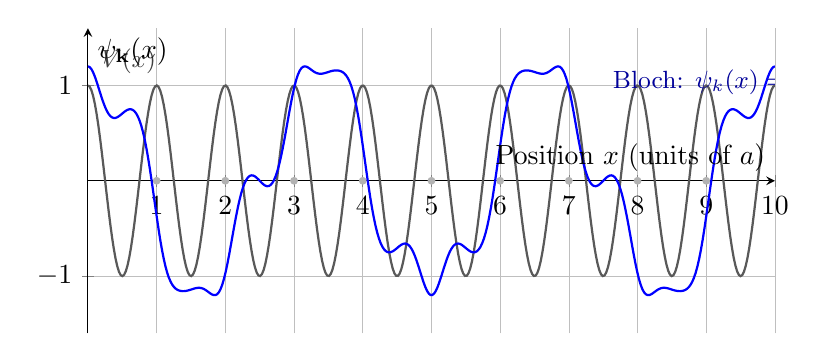
\begin{tikzpicture}
\begin{axis}[
    width=0.85\textwidth,
    height=0.45\textwidth,
    xlabel={Position $x$ (units of $a$)},
    ylabel={$\psi_{\vb{k}}(x)$},
    xmin=0, xmax=10,
    ymin=-1.6, ymax=1.6,
    grid=both,
    grid style={line width=.1pt, draw=gray!20},
    major grid style={line width=.2pt,draw=gray!50},
    axis lines=middle,
    samples=400,
]
% Lattice sites
\pgfplotsinvokeforeach{1,2,...,9}{
    \node[circle,fill=gray!60,inner sep=1.0pt] at (axis cs:#1, 0) {};
}
% Periodic potential
\addplot[gray!70!black, thick, domain=0:10, samples=400] {1.0*cos(deg(2*pi*x))};
\node[anchor=west, gray!50!black, font=\small] at (axis cs:0.05, 1.25) {$V(x)$};
% Bloch wave (real part) - k not at zone boundary (k=0.3 pi/a)
\addplot[blue, thick, domain=0:10, samples=400] {1.2*cos(deg(0.3*2*pi*x + 0.4*sin(deg(2*pi*x))))};
\node[anchor=west, blue!60!black, font=\small] at (axis cs:7.5, 1.05) {Bloch: $\psi_k(x)=e^{ikx}u_k(x)$};
\end{axis}
\end{tikzpicture}
\caption{Real part of a 1D Bloch wave (blue) in a weak periodic potential $V(x)$ (gray). The wave is a plane wave $e^{ikx}$ modulated by a lattice-periodic function $u_k(x)$ with the same period $a$ as the potential. This is the general form of eigenstates in a crystal.}
\label{fig:bloch}
\end{figure}

\subsection{Physical Nature of Crystal Momentum $\hbar\vb{k}$}
In free space, an electron with wavefunction $\psi = e^{i\vb{k}\cdot\vb{r}}$ has a definite kinematic momentum $\hat{\vb{p}}\psi = -i\hbar\nabla\psi = \hbar\vb{k}\psi$.

In a crystalline potential, however, a Bloch wave is NOT an eigenstate of true momentum $\hat{\vb{p}}$:
\begin{equation}
-i\hbar\nabla \psi_{n\vb{k}}(\vb{r}) = -i\hbar\nabla\left[ e^{i\vb{k}\cdot\vb{r}}u_{n\vb{k}}(\vb{r}) \right] = \hbar\vb{k}\psi_{n\vb{k}}(\vb{r}) + e^{i\vb{k}\cdot\vb{r}}(-i\hbar\nabla u_{n\vb{k}}(\vb{r})) \neq \text{const} \times \psi_{n\vb{k}}(\vb{r})
\end{equation}
The electron continuously exchanges linear momentum with the periodic array of ion cores. The vector $\hbar\vb{k}$ is called the \textbf{crystal momentum}. It acts as an effective quantum number governing the translational symmetry of the wavepacket.

\paragraph{Conservation Modulo Reciprocal Lattice Vectors:}
Let $\vb{G}$ be any reciprocal lattice vector satisfying $e^{i\vb{G}\cdot\vb{R}} = 1$ for all direct lattice vectors $\vb{R}$. Under lattice translation:
\begin{equation}
\psi_{\vb{k}+\vb{G}}(\vb{r}+\vb{R}) = e^{i(\vb{k}+\vb{G})\cdot\vb{R}}\psi_{\vb{k}+\vb{G}}(\vb{r}) = e^{i\vb{k}\cdot\vb{R}}e^{i\vb{G}\cdot\vb{R}}\psi_{\vb{k}+\vb{G}}(\vb{r}) = e^{i\vb{k}\cdot\vb{R}}\psi_{\vb{k}+\vb{G}}(\vb{r})
\end{equation}
The phase factor $e^{i\vb{k}\cdot\vb{R}}$ is completely unchanged if $\vb{k}$ is replaced by $\vb{k} + \vb{G}$! 

Therefore, wavevectors that differ by a reciprocal lattice vector are physically equivalent:
\begin{equation}
\boxed{\vb{k} \equiv \vb{k} + \vb{G}}
\end{equation}
In all quantum scattering events in crystals (such as electron--phonon or electron--photon collisions), total crystal momentum is conserved \textbf{modulo $\vb{G}$}:
\begin{equation}
\vb{k}_1 + \vb{k}_2 = \vb{k}_3 + \vb{k}_4 + \vb{G}
\end{equation}
When $\vb{G} = \vb{0}$, the event is a \emph{Normal process} ($N$-process). When $\vb{G} \neq \vb{0}$, the event is an \emph{Umklapp process} ($U$-process), where the crystal lattice as a whole recoils by momentum $\hbar\vb{G}$.

\subsection{Born--von Karman Boundary Conditions and State Counting}
To enumerate allowed $\vb{k}$-states, we apply Born--von Karman periodic boundary conditions across a macroscopic crystal containing $N_1 \times N_2 \times N_3 = N_c$ unit cells:
\begin{equation}
\psi(\vb{r} + N_i \vb{a}_i) = \psi(\vb{r}) \implies e^{i N_i \vb{k}\cdot\vb{a}_i} = 1 \implies \vb{k}\cdot\vb{a}_i = \frac{2\pi m_i}{N_i}, \quad m_i \in \mathbb{Z}
\end{equation}
Expanding $\vb{k}$ in the primitive reciprocal basis vectors $\vb{b}_1, \vb{b}_2, \vb{b}_3$ (where $\vb{a}_i \cdot \vb{b}_j = 2\pi\delta_{ij}$):
\begin{equation}
\vb{k} = \frac{m_1}{N_1}\vb{b}_1 + \frac{m_2}{N_2}\vb{b}_2 + \frac{m_3}{N_3}\vb{b}_3
\label{eq:k_grid_bvk}
\end{equation}
The volume occupied by a single $\vb{k}$-state in reciprocal space is:
\begin{equation}
\Delta V_k = \frac{\vb{b}_1 \cdot (\vb{b}_2 \times \vb{b}_3)}{N_1 N_2 N_3} = \frac{V_{\mathrm{BZ}}}{N_c}
\end{equation}
where $V_{\mathrm{BZ}} = \frac{(2\pi)^3}{V_{\mathrm{cell}}}$ is the total volume of the \textbf{first Brillouin zone}.

Consequently, the total number of distinct allowed wavevector states within the first Brillouin zone is:
\begin{equation}
\frac{V_{\mathrm{BZ}}}{\Delta V_k} = N_c
\end{equation}
Each orbital state accommodates two electrons of opposite spin ($g_s = 2$). We arrive at a central theorem of solid-state physics:
\begin{equation}
\boxed{\text{Each non-degenerate energy band can accommodate at most } 2N_c \text{ electrons}}
\label{eq:band_capacity_2Nc}
\end{equation}

\subsection{The Three Zone Schemes}
Because $E_n(\vb{k} + \vb{G}) = E_n(\vb{k})$, the band dispersion $E(\vb{k})$ can be graphically represented in three standard schemes:
\begin{enumerate}[leftmargin=*]
    \item \textbf{Extended Zone Scheme}: Different energy bands are plotted in different Brillouin zones. Band $1$ is plotted in the 1st BZ ($|k| \le \pi/a$), Band $2$ in the 2nd BZ ($\pi/a < |k| \le 2\pi/a$), Band $3$ in the 3rd BZ, and so on. In the limit of zero crystal potential ($V \to 0$), the dispersion forms a continuous free-electron parabola $E = \hbar^2 k^2 / 2m_e$.
    \item \textbf{Reduced Zone Scheme}: All energy bands are mapped back into the first Brillouin zone ($-\pi/a \le k \le \pi/a$) by translating wavevectors by appropriate reciprocal lattice vectors $\vb{G}$. In this scheme, the energy dispersion is multi-valued: for each $\vb{k}$ in the 1st BZ, there exists an infinite ladder of discrete energy eigenvalues $E_n(\vb{k})$ labeled by band index $n = 1, 2, 3, \dots$.
    \item \textbf{Periodic (Repeated) Zone Scheme}: The energy bands in the first Brillouin zone are repeated periodically throughout all reciprocal space by adding $\vb{G}$ in all directions. This scheme is particularly useful for visualizing electron orbits and cyclotron trajectories across multiple zones in magnetic fields.
\end{enumerate}

\begin{figure}[h]
\centering
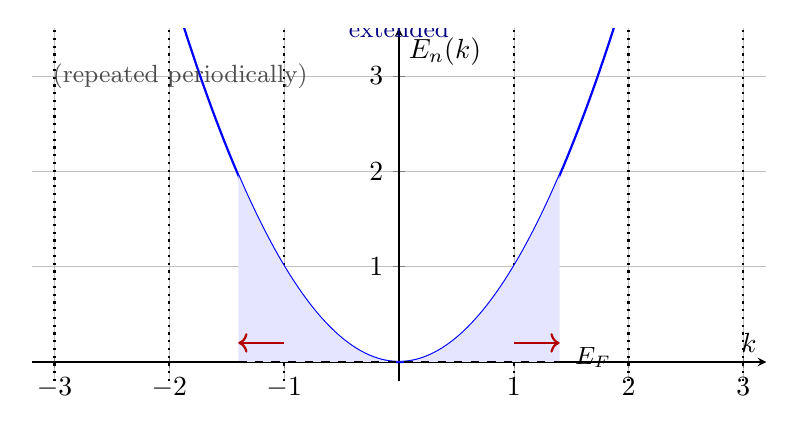
\begin{tikzpicture}
% Three identical panels: extended / reduced / repeated zones, schematic E(k)
% Draw a 1D parabolic band in each zone piece
\begin{axis}[
    width=0.9\textwidth,
    height=0.5\textwidth,
    xlabel={$k$},
    ylabel={$E_n(k)$},
    xmin=-3.2, xmax=3.2,
    ymin=-0.2, ymax=3.5,
    grid=both,
    grid style={line width=.1pt, draw=gray!20},
    major grid style={line width=.2pt,draw=gray!50},
    axis lines=middle,
    samples=200,
]
% Zone boundaries
\foreach \xb in {-3,-2,-1,1,2,3}{
    \addplot[black, dotted, thick] coordinates {(\xb, -0.2) (\xb, 3.5)};
}
% Extended-zone: 3 parabolas centered at k=0, +/-2
\addplot[blue, thick, domain=-3.2:3.2] {x^2};
\addplot[blue, thick, domain=-1:1] {4 + 0.6*(x-1)^2};
\node[anchor=south, blue!50!black, font=\small] at (axis cs:0, 3.3) {extended};

% Filled lower band (extended) up to EF
\addplot[blue, fill=blue!10, draw=none, domain=-1.4:1.4, samples=100] {x^2} \closedcycle;
\addplot[black, dashed] coordinates {(-1.4, 0) (1.4, 0)};
\node[anchor=west, font=\small] at (axis cs:1.45, 0.05) {$E_F$};

% Highlight 1st BZ
\draw[red!70!black, thick, ->] (axis cs:-1, 0.2) -- (axis cs:-1.4, 0.2);
\draw[red!70!black, thick, ->] (axis cs:1, 0.2) -- (axis cs:1.4, 0.2);
\node[red!70!black, font=\small\bfseries] at (axis cs:0, -0.6) {1st Brillouin zone};

% Repeated-zone indicator: 3 copies
\node[anchor=west, font=\small, gray!60!black] at (axis cs:-3.1, 3.0) {(repeated periodically)};
\end{axis}
\end{tikzpicture}
\caption{Extended-zone scheme: the free-electron parabola $E=\hbar^2k^2/2m_e$ is plotted for all $k$. Allowed $k$ values from Born--von Karman BCs, the first Brillouin zone, and the filled states up to $E_F$ are shown. The same dispersion can be folded into the first BZ (reduced zone) or copied periodically (repeated zone).}
\label{fig:zone_schemes}
\end{figure}

\begin{checkpointbox}{Why Crystal Momentum $\hbar\vb{k}$ is Not True Momentum}
True momentum is a continuous translation generator; crystal momentum is a discrete translation generator. 

When an external force $\vb{F}_{\mathrm{ext}}$ acts on a Bloch electron, the semiclassical equation of motion is $\hbar \frac{d\vb{k}}{dt} = \vb{F}_{\mathrm{ext}}$. Although this equation mirrors Newton's second law, $\hbar\vb{k}$ is NOT the mechanical momentum of the electron. The actual physical momentum of the electron is continuously modulated by the periodic forces exerted by the lattice ions. When an electron is accelerated to a Brillouin zone boundary $k = \pi/a$, it undergoes Bragg reflection back to $-\pi/a$, transferring an impulse of $\hbar G = 2\pi\hbar/a$ directly to the entire crystal lattice.
\end{checkpointbox}

\begin{takeawaybox}{State Counting in Brillouin Zones}
The fact that each energy band accommodates exactly $2N_c$ electrons (with spin) leads directly to the fundamental classification of solids:
\begin{itemize}
    \item \textbf{Odd Valency}: If a crystal has an \emph{odd} number of valence electrons per primitive unit cell (e.g., alkali metals Li, Na, K with $1$, or noble metals Cu, Ag, Au with $1$), the highest occupied band can be at most half-filled. The material \textbf{must be a metal}!
    \item \textbf{Even Valency}: If a crystal has an \emph{even} number of valence electrons per unit cell (e.g., diamond with $8$ electrons per primitive cell), bands can be completely filled. If a finite energy gap $E_g$ separates the highest filled band (valence band) from the lowest empty band (conduction band), the material is an \textbf{insulator} or \textbf{semiconductor}.
\end{itemize}
\end{takeawaybox}

\vspace{0.4cm}

% -------------------------------------------------------------------------
% SOLVED EXAMPLE FOR CHAPTER 8
% -------------------------------------------------------------------------
\begin{examplebox}{Free Electron Plane Wave as a Trivial Bloch State}{ex:free_plane_bloch}
\textbf{Problem Statement:}
Show that a standard free-electron plane wave $\psi_{\vb{k}}(\vb{r}) = \frac{1}{\sqrt{V}}e^{i\vb{k}\cdot\vb{r}}$ satisfies Bloch's theorem for an arbitrary periodic lattice with translation vector $\vb{R}$. Identify the cell-periodic function $u_{\vb{k}}(\vb{r})$ and verify that it possesses the required lattice periodicity.

\vspace{0.2cm}\hrule\vspace{0.2cm}
\textbf{Step-by-Step Solution:}

\textbf{1. Verification of the First Bloch Formulation:}
Evaluate $\psi_{\vb{k}}(\vb{r} + \vb{R})$:
\[
\psi_{\vb{k}}(\vb{r} + \vb{R}) = \frac{1}{\sqrt{V}}e^{i\vb{k}\cdot(\vb{r}+\vb{R})} = e^{i\vb{k}\cdot\vb{R}}\left[ \frac{1}{\sqrt{V}}e^{i\vb{k}\cdot\vb{r}} \right] = e^{i\vb{k}\cdot\vb{R}}\psi_{\vb{k}}(\vb{r})
\]
This satisfies equation~\eqref{eq:bloch_statement_1} identically!

\textbf{2. Identification of $u_{\vb{k}}(\vb{r})$:}
Comparing $\psi_{\vb{k}}(\vb{r}) = e^{i\vb{k}\cdot\vb{r}}u_{\vb{k}}(\vb{r})$ with the plane wave:
\[
e^{i\vb{k}\cdot\vb{r}}u_{\vb{k}}(\vb{r}) = \frac{1}{\sqrt{V}}e^{i\vb{k}\cdot\vb{r}} \implies u_{\vb{k}}(\vb{r}) = \frac{1}{\sqrt{V}} = \mathrm{constant}
\]

\textbf{3. Verification of Cell Periodicity:}
Since $u_{\vb{k}}(\vb{r})$ is a spatially uniform constant:
\[
u_{\vb{k}}(\vb{r} + \vb{R}) = \frac{1}{\sqrt{V}} = u_{\vb{k}}(\vb{r})
\]
A spatially constant function trivially satisfies the lattice periodicity requirement $u(\vb{r}+\vb{R}) = u(\vb{r})$ for any arbitrary lattice vector $\vb{R}$. Thus, free electrons are merely the special limiting case of Bloch electrons in a vanishing crystal potential ($V(\vb{r}) \to 0$).
\end{examplebox}

\clearpage


% =========================================================================
% CHAPTER 9: NEARLY FREE ELECTRON MODEL & ENERGY GAPS
% =========================================================================
\section{Nearly Free Electron Model and Energy Gaps}
\label{sec:nearly_free_electron}

\subsection{Perturbation Theory for a Weak Periodic Potential}
In the \textbf{Nearly Free Electron} (NFE) model, we treat the lattice-periodic potential $V(\vb{r})$ as a weak perturbation on an otherwise free electron gas:
\begin{equation}
\hat{H} = \hat{H}_0 + V(\vb{r}) = -\frac{\hbar^2}{2m_e}\nabla^2 + V(\vb{r})
\end{equation}
Because $V(\vb{r} + \vb{R}) = V(\vb{r})$, it can be expanded in a three-dimensional complex Fourier series over all reciprocal lattice vectors $\vb{G}$:
\begin{equation}
V(\vb{r}) = \sum_{\vb{G}} V_{\vb{G}} e^{i\vb{G}\cdot\vb{r}}
\label{eq:fourier_potential}
\end{equation}
where the Fourier coefficients $V_{\vb{G}}$ are given by the unit cell integral:
\begin{equation}
V_{\vb{G}} = \frac{1}{V_{\mathrm{cell}}}\int_{\mathrm{cell}} V(\vb{r}) e^{-i\vb{G}\cdot\vb{r}}\,d^3r
\end{equation}
Because $V(\vb{r})$ is real ($V^*(\vb{r}) = V(\vb{r})$), the Fourier amplitudes satisfy $V_{-\vb{G}} = V_{\vb{G}}^*$. We can choose the arbitrary reference zero of potential energy such that the spatial average vanishes: $V_0 = 0$.

\subsection{Matrix Elements and Selection Rules}
Using normalized free-electron plane waves $|\vb{k}\rangle = \frac{1}{\sqrt{V}}e^{i\vb{k}\cdot\vb{r}}$ as the unperturbed basis:
\begin{align}
\langle \vb{k}' | V | \vb{k} \rangle &= \frac{1}{V}\int_V e^{-i\vb{k}'\cdot\vb{r}} \left[ \sum_{\vb{G}} V_{\vb{G}} e^{i\vb{G}\cdot\vb{r}} \right] e^{i\vb{k}\cdot\vb{r}}\,d^3r \nonumber \\
&= \sum_{\vb{G}} V_{\vb{G}} \left[ \frac{1}{V}\int_V e^{i(\vb{k} - \vb{k}' + \vb{G})\cdot\vb{r}}\,d^3r \right] = \sum_{\vb{G}} V_{\vb{G}} \delta_{\vb{k}',\vb{k}+\vb{G}}
\label{eq:matrix_element_selection}
\end{align}
This is a powerful selection rule: \textbf{the periodic potential couples only plane-wave states whose wavevectors differ by a reciprocal lattice vector $\vb{G}$}.

\subsection{Non-Degenerate Perturbation Theory and its Breakdown}
In standard Rayleigh--Schrödinger non-degenerate perturbation theory, the energy of state $|\vb{k}\rangle$ to second order is:
\begin{equation}
E(\vb{k}) = E^{(0)}(\vb{k}) + \langle \vb{k}|V|\vb{k}\rangle + \sum_{\vb{k}' \neq \vb{k}} \frac{|\langle \vb{k}'|V|\vb{k}\rangle|^2}{E^{(0)}(\vb{k}) - E^{(0)}(\vb{k}')}
\end{equation}
Applying the selection rule~\eqref{eq:matrix_element_selection} and setting $\langle\vb{k}|V|\vb{k}\rangle = V_0 = 0$:
\begin{equation}
E(\vb{k}) = E^{(0)}(\vb{k}) + \sum_{\vb{G} \neq \vb{0}} \frac{|V_{\vb{G}}|^2}{E^{(0)}(\vb{k}) - E^{(0)}(\vb{k}+\vb{G})}
\label{eq:second_order_pt}
\end{equation}
where $E^{(0)}(\vb{k}) = \frac{\hbar^2 k^2}{2m_e}$.

\paragraph{Breakdown at Zone Boundaries:}
Equation~\eqref{eq:second_order_pt} is valid as long as the denominator is large: $|E^{(0)}(\vb{k}) - E^{(0)}(\vb{k}+\vb{G})| \gg |V_{\vb{G}}|$. 

However, whenever the unperturbed energies of $|\vb{k}\rangle$ and $|\vb{k}+\vb{G}\rangle$ become equal:
\begin{equation}
E^{(0)}(\vb{k}) = E^{(0)}(\vb{k}+\vb{G}) \iff k^2 = |\vb{k}+\vb{G}|^2 = k^2 + 2\vb{k}\cdot\vb{G} + G^2
\end{equation}
the denominator vanishes ($E^{(0)}(\vb{k}) - E^{(0)}(\vb{k}+\vb{G}) = 0$) and the energy correction diverges to infinity! 

Canceling $k^2$ gives the geometric condition for degeneracy:
\begin{equation}
2\vb{k}\cdot\vb{G} + G^2 = 0 \iff \boxed{\vb{k}\cdot\left(\frac{1}{2}\vb{G}\right) = -\frac{1}{4}G^2 \iff \vb{G}\cdot\left(\vb{k} + \frac{1}{2}\vb{G}\right) = 0}
\label{eq:bragg_condition}
\end{equation}
Equation~\eqref{eq:bragg_condition} is the exact mathematical definition of the \textbf{Brillouin zone boundary}! It is precisely the Laue condition for the constructive Bragg reflection of an electron de Broglie wave by the crystal planes perpendicular to $\vb{G}$.

\subsection{Degenerate Perturbation Theory and the $2\times 2$ Secular Equation}
Near a Brillouin zone boundary where $|\vb{k}\rangle$ and $|\vb{k}+\vb{G}\rangle$ are nearly degenerate, non-degenerate perturbation theory must be replaced by \textbf{degenerate perturbation theory}. We construct a trial Bloch wavefunction as a linear superposition of the two strongly coupled states:
\begin{equation}
\psi(\vb{r}) = c_1 |\vb{k}\rangle + c_2 |\vb{k}+\vb{G}\rangle = c_1 \frac{1}{\sqrt{V}}e^{i\vb{k}\cdot\vb{r}} + c_2 \frac{1}{\sqrt{V}}e^{i(\vb{k}+\vb{G})\cdot\vb{r}}
\label{eq:two_wave_superposition}
\end{equation}
Substituting this trial function into the Schrödinger equation $\hat{H}\psi = E\psi$:
\begin{equation}
(\hat{H}_0 + V) \left( c_1 |\vb{k}\rangle + c_2 |\vb{k}+\vb{G}\rangle \right) = E \left( c_1 |\vb{k}\rangle + c_2 |\vb{k}+\vb{G}\rangle \right)
\end{equation}
Projecting successively onto $\langle \vb{k}|$ and $\langle \vb{k}+\vb{G}|$:
\begin{align}
\left( E^{(0)}(\vb{k}) - E \right) c_1 + V_{\vb{G}}^* c_2 &= 0 \\
V_{\vb{G}} c_1 + \left( E^{(0)}(\vb{k}+\vb{G}) - E \right) c_2 &= 0
\end{align}
For non-trivial coefficients $(c_1, c_2) \neq (0, 0)$, the determinant of the coefficients must vanish, yielding the fundamental \textbf{$2\times 2$ Secular Equation}:
\begin{equation}
\begin{vmatrix}
E^{(0)}(\vb{k}) - E & V_{\vb{G}}^* \\
V_{\vb{G}} & E^{(0)}(\vb{k}+\vb{G}) - E
\end{vmatrix} = 0
\label{eq:secular_determinant}
\end{equation}
Expanding the determinant:
\begin{equation}
\left( E^{(0)}(\vb{k}) - E \right)\left( E^{(0)}(\vb{k}+\vb{G}) - E \right) - |V_{\vb{G}}|^2 = 0
\label{eq:secular_quadratic}
\end{equation}
Solving this quadratic equation for the two energy eigenvalues $E_\pm$:
\begin{equation}
E_\pm(\vb{k}) = \frac{E^{(0)}(\vb{k}) + E^{(0)}(\vb{k}+\vb{G})}{2} \pm \sqrt{ \left( \frac{E^{(0)}(\vb{k}) - E^{(0)}(\vb{k}+\vb{G})}{2} \right)^2 + |V_{\vb{G}}|^2 }
\label{eq:nfe_eigenvalues_full}
\end{equation}

\subsection{Energy Band Gap at the Brillouin Zone Boundary}
Directly at the Brillouin zone boundary, the two unperturbed plane-wave energies are degenerate:
\begin{equation}
E^{(0)}(\vb{k}) = E^{(0)}(\vb{k}+\vb{G}) \equiv E_0 = \frac{\hbar^2 k_0^2}{2m_e} = \frac{\hbar^2 (G/2)^2}{2m_e}
\end{equation}
The square root in equation~\eqref{eq:nfe_eigenvalues_full} simplifies cleanly:
\begin{equation}
E_\pm = E_0 \pm \sqrt{0 + |V_{\vb{G}}|^2} = E_0 \pm |V_{\vb{G}}|
\end{equation}
The single unperturbed energy level $E_0$ splits into two separate energy levels:
\begin{itemize}
    \item Lower band energy: $E_- = E_0 - |V_{\vb{G}}|$
    \item Upper band energy: $E_+ = E_0 + |V_{\vb{G}}|$
\end{itemize}
The forbidden \textbf{energy band gap} $\Delta E = E_g$ opened by the periodic potential is:
\begin{equation}
\boxed{E_g = \Delta E = E_+ - E_- = 2|V_{\vb{G}}|}
\label{eq:band_gap_formula}
\end{equation}
The magnitude of the energy band gap at any Brillouin zone boundary is \textbf{exactly twice the absolute value of the corresponding Fourier component of the crystal potential}!

\begin{figure}[h]
\centering
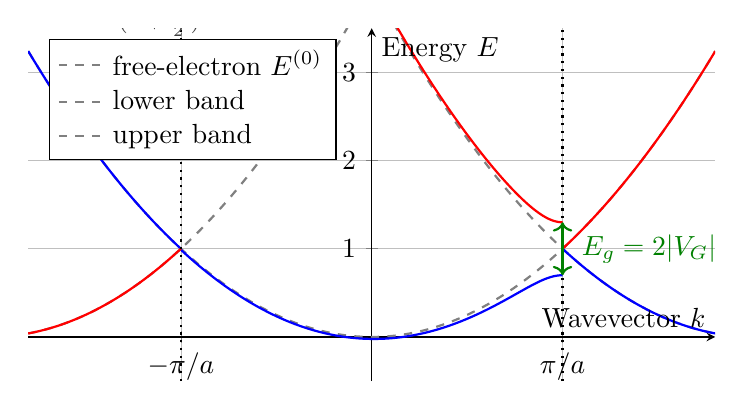
\begin{tikzpicture}
\begin{axis}[
    width=0.85\textwidth,
    height=0.5\textwidth,
    xlabel={Wavevector $k$},
    ylabel={Energy $E$},
    xmin=-1.8, xmax=1.8,
    ymin=-0.5, ymax=3.5,
    legend pos=north west,
    legend cell align=left,
    grid=both,
    grid style={line width=.1pt, draw=gray!20},
    major grid style={line width=.2pt,draw=gray!50},
    axis lines=middle,
    xtick={-1, 1},
    xticklabels={$-\pi/a$, $\pi/a$},
    samples=200,
]
% Free electron parabolas
\addplot[gray, dashed, thick, domain=-1.8:1.8] {x^2};
\addplot[gray, dashed, thick, domain=-1.8:1.8] {(x-2)^2};
\addplot[gray, dashed, thick, domain=-1.8:1.8] {(x+2)^2};
\addlegendentry{free-electron $E^{(0)}$}

% NFE bands with gap (Lower band)
\addplot[blue, thick, domain=-1.8:-1, samples=50] {x^2};
\addplot[blue, thick, domain=-1:1] { (x^2 + (x-2)^2)/2 - sqrt( ((x^2 - (x-2)^2)/2)^2 + 0.09 ) };
\addplot[blue, thick, domain=1:1.8, samples=50] {(x-2)^2};
\addlegendentry{lower band}

% NFE bands with gap (Upper band)
\addplot[red, thick, domain=-1.8:-1, samples=50] {(x+2)^2};
\addplot[red, thick, domain=-1:1] { (x^2 + (x-2)^2)/2 + sqrt( ((x^2 - (x-2)^2)/2)^2 + 0.09 ) };
\addplot[red, thick, domain=1:1.8, samples=50] {x^2};
\addlegendentry{upper band}

% Zone boundary lines
\addplot[black, dotted, thick] coordinates {(-1, -0.5) (-1, 3.5)};
\addplot[black, dotted, thick] coordinates {(1, -0.5) (1, 3.5)};
\node[anchor=south, font=\small] at (axis cs:1, 3.4) {BZ boundary};

% Gap annotation
\draw[<->, thick, green!50!black] (axis cs: 1, 0.7) -- (axis cs: 1, 1.3);
\node[anchor=west, font=\bfseries, green!50!black] at (axis cs: 1.05, 1.0) {$E_g = 2|V_G|$};

% Bragg condition label
\node[anchor=south east, font=\small, gray!50!black] at (axis cs:-0.6, 3.3) {$\vb{G}\!\cdot\!(\vb{k}\!+\!\tfrac{\vb{G}}{2})=0$};
\end{axis}
\end{tikzpicture}
\caption{Nearly free electron band structure near the first Brillouin-zone boundary ($k = \pm \pi/a$). The dashed gray lines show the free-electron parabolas $E^{(0)}$, and the solid blue/red curves show the avoided crossing that opens an energy gap $E_g = 2|V_G|$ at the Bragg condition $\vb{G}\cdot(\vb{k}+\vb{G}/2)=0$.}
\label{fig:nfe_band}
\end{figure}

\subsection{Physical Origin of the Band Gap: Standing Wave Electrostatics}
Why does a weak periodic potential split the energy spectrum into allowed bands and forbidden band gaps? 

At the zone boundary in 1D ($k = \pm \pi/a$ with $G = -2\pi/a$), the forward-traveling wave $e^{i\pi x/a}$ and backward-traveling wave $e^{-i\pi x/a}$ have identical amplitudes. Instead of traveling waves, Bragg reflection locks them into two orthogonal \textbf{stationary standing waves}:
\begin{align}
\psi_+(x) &= \frac{1}{\sqrt{2}}\left( e^{i\pi x/a} + e^{-i\pi x/a} \right) = \sqrt{2}\cos\left(\frac{\pi x}{a}\right) \label{eq:psi_plus} \\
\psi_-(x) &= \frac{1}{\sqrt{2}i}\left( e^{i\pi x/a} - e^{-i\pi x/a} \right) = \sqrt{2}\sin\left(\frac{\pi x}{a}\right) \label{eq:psi_minus}
\end{align}
Now examine the spatial probability densities of these two standing waves:
\begin{align}
\rho_+(x) &= |\psi_+(x)|^2 = 2\cos^2\left(\frac{\pi x}{a}\right) = 1 + \cos\left(\frac{2\pi x}{a}\right) \label{eq:rho_plus} \\
\rho_-(x) &= |\psi_-(x)|^2 = 2\sin^2\left(\frac{\pi x}{a}\right) = 1 - \cos\left(\frac{2\pi x}{a}\right) \label{eq:rho_minus}
\end{align}
Assume the positive ion cores are located at lattice sites $x = 0, \pm a, \pm 2a, \dots$, where the attractive potential energy $V(x) \approx -V_0\cos(2\pi x/a)$ is at its most negative:
\begin{enumerate}
    \item \textbf{Wavefunction $\psi_+$}: The charge density $\rho_+(x)$ peaks at $x = 0, \pm a, \dots$, concentrating the negative electron charge \textbf{directly on top of the positive ion cores}. The attractive Coulomb interaction is maximized, \textbf{lowering the potential energy}:
    \begin{equation}
    \langle V \rangle_+ = \int_0^a \rho_+(x) V(x)\,dx = \int_0^a \left[1 + \cos\left(\frac{2\pi x}{a}\right)\right]\left[-V_0\cos\left(\frac{2\pi x}{a}\right)\right]dx = -\frac{V_0}{2}
    \end{equation}
    \item \textbf{Wavefunction $\psi_-$}: The charge density $\rho_-(x)$ vanishes at the ion cores ($x=0$) and peaks midway between the cores ($x = \pm a/2$), piling electron charge in the regions of weakest attraction, \textbf{raising the potential energy}:
    \begin{equation}
    \langle V \rangle_- = \int_0^a \rho_-(x) V(x)\,dx = \int_0^a \left[1 - \cos\left(\frac{2\pi x}{a}\right)\right]\left[-V_0\cos\left(\frac{2\pi x}{a}\right)\right]dx = +\frac{V_0}{2}
    \end{equation}
\end{enumerate}
The difference in electrostatic potential energy between these two charge distributions is:
\begin{equation}
\Delta E = \langle V \rangle_- - \langle V \rangle_+ = +\frac{V_0}{2} - \left(-\frac{V_0}{2}\right) = V_0 = 2|V_G|
\end{equation}
The energy band gap is not an abstract mathematical artifact: \textbf{it is the electrostatic potential energy difference between an electron cloud that clusters on positive ion cores versus an electron cloud that clusters between them!}

\begin{checkpointbox}{Physical Intuition for Energy Gap Formation}
At any wavevector $k$ far from zone boundaries, an electron wavepacket travels smoothly through the crystal with uniform probability density $|\psi|^2 = 1/V$, sampling the attractive and repulsive regions equally. 

At the zone boundary, Bragg reflection creates stationary nodes. If the electron puts its charge antinodes on the positive ions, its energy drops; if it puts its antinodes between the ions, its energy rises. No stationary quantum state can exist with an energy intermediate between these two configurations: hence, an energy gap opens!
\end{checkpointbox}

\begin{methodbox}{Setting Up the Secular Determinant at Zone Boundaries}
For any weak crystal potential $V(\vb{r})$:
\begin{enumerate}
    \item Identify the Brillouin zone boundary of interest (e.g., $k = \pm \pi/a$ with $G = 2\pi/a$).
    \item Compute the Fourier transform of the crystal potential for that reciprocal lattice vector:
    \[
    V_{\vb{G}} = \frac{1}{V_{\mathrm{cell}}}\int_{\mathrm{cell}} V(\vb{r}) e^{-i\vb{G}\cdot\vb{r}}\,d^3r
    \]
    \item The band gap opened at that specific zone boundary is immediately given by $\Delta E = 2|V_{\vb{G}}|$.
    \item The unperturbed kinetic energy at the boundary is $E_0 = \frac{\hbar^2 (G/2)^2}{2m_e}$.
    \item The band edges are $E_{\mathrm{lower}} = E_0 - |V_{\vb{G}}|$ and $E_{\mathrm{upper}} = E_0 + |V_{\vb{G}}|$.
\end{enumerate}
\end{methodbox}

\vspace{0.4cm}

% -------------------------------------------------------------------------
% SOLVED EXAMPLES FOR CHAPTER 9
% -------------------------------------------------------------------------
\begin{examplebox}{Exact Solution of the $2\times 2$ Zone-Boundary Secular Equation}{ex:secular_solution}
\textbf{Problem Statement:}
Consider a 1D lattice with potential $V(x) = V_0 \cos(2\pi x/a)$ where $V_0 = 1.20\ \mathrm{eV}$ and lattice constant $a = 3.00\ \text{\AA}$.
\begin{enumerate}[label=(\alph*)]
    \item Find the Fourier components $V_G$ for $G = \pm 2\pi/a$.
    \item Calculate the unperturbed kinetic energy $E_0$ at the zone boundary $k = \pi/a$.
    \item Determine the upper and lower band edge energies and the band gap $\Delta E$.
\end{enumerate}

\vspace{0.2cm}\hrule\vspace{0.2cm}
\textbf{Step-by-Step Solution:}

\textbf{(a) Fourier components:}
Using Euler's identity:
\[
V(x) = V_0 \cos\left(\frac{2\pi x}{a}\right) = \frac{V_0}{2}e^{i(2\pi/a)x} + \frac{V_0}{2}e^{-i(2\pi/a)x}
\]
Comparing with $V(x) = \sum_G V_G e^{i G x}$, the non-zero Fourier components are:
\[
V_{2\pi/a} = V_{-2\pi/a} = \frac{V_0}{2} = \frac{1.20\ \mathrm{eV}}{2} = \mathbf{0.60\ \mathrm{eV}}
\]

\textbf{(b) Unperturbed energy $E_0$ at $k = \pi/a$:}
\[
k_0 = \frac{\pi}{a} = \frac{\pi}{3.00 \times 10^{-10}\ \mathrm{m}} \approx 1.047 \times 10^{10}\ \mathrm{m^{-1}}
\]
\begin{align*}
E_0 &= \frac{\hbar^2 k_0^2}{2m_e} = \frac{(1.0546 \times 10^{-34}\ \mathrm{J\cdot s})^2 (1.047 \times 10^{10}\ \mathrm{m^{-1}})^2}{2(9.109 \times 10^{-31}\ \mathrm{kg})} \\
&= \frac{1.220 \times 10^{-48}}{1.822 \times 10^{-30}} \approx 6.697 \times 10^{-19}\ \mathrm{J} = \frac{6.697 \times 10^{-19}\ \mathrm{J}}{1.6022 \times 10^{-19}\ \mathrm{J/eV}} \approx \mathbf{4.18\ \mathrm{eV}}
\end{align*}

\textbf{(c) Band edge energies and band gap:}
\begin{align*}
E_- &= E_0 - |V_G| = 4.18\ \mathrm{eV} - 0.60\ \mathrm{eV} = \mathbf{3.58\ \mathrm{eV}} \\
E_+ &= E_0 + |V_G| = 4.18\ \mathrm{eV} + 0.60\ \mathrm{eV} = \mathbf{4.78\ \mathrm{eV}} \\
\Delta E &= 2|V_G| = 2(0.60\ \mathrm{eV}) = \mathbf{1.20\ \mathrm{eV}}
\end{align*}
\end{examplebox}

\vspace{0.4cm}

\begin{examplebox}{Coulomb Energy Difference of Zone-Boundary Standing Waves}{ex:standing_waves_energy}
\textbf{Problem Statement:}
For a 1D lattice potential $V(x) = -V_0 \cos(2\pi x/a)$ with $V_0 > 0$, calculate the first-order perturbation energy shift $\Delta E_\pm = \langle \psi_\pm | V | \psi_\pm \rangle$ for the two normalized standing waves:
\[
\psi_+(x) = \sqrt{\frac{2}{L}}\cos\left(\frac{\pi x}{a}\right), \quad \psi_-(x) = \sqrt{\frac{2}{L}}\sin\left(\frac{\pi x}{a}\right)
\]
and verify that the resulting splitting reproduces the band gap $\Delta E = 2|V_G|$.

\vspace{0.2cm}\hrule\vspace{0.2cm}
\textbf{Step-by-Step Solution:}

The expectation value of the potential energy is:
\[
\langle V \rangle_+ = \int_0^L |\psi_+(x)|^2 V(x)\,dx = \frac{2}{L}\int_0^L \cos^2\left(\frac{\pi x}{a}\right)\left[-V_0 \cos\left(\frac{2\pi x}{a}\right)\right]dx
\]
Using the trigonometric identity $\cos^2\theta = \frac{1 + \cos(2\theta)}{2}$:
\begin{align*}
\langle V \rangle_+ &= -\frac{V_0}{L}\int_0^L \left[1 + \cos\left(\frac{2\pi x}{a}\right)\right]\cos\left(\frac{2\pi x}{a}\right)dx \\
&= -\frac{V_0}{L}\left[ \int_0^L \cos\left(\frac{2\pi x}{a}\right)dx + \int_0^L \cos^2\left(\frac{2\pi x}{a}\right)dx \right]
\end{align*}
Over an integer number of unit cells ($L = N a$), $\int_0^L \cos(2\pi x/a)dx = 0$, and $\int_0^L \cos^2(2\pi x/a)dx = L/2$.
Thus:
\[
\langle V \rangle_+ = -\frac{V_0}{L}\left( 0 + \frac{L}{2} \right) = \mathbf{-\frac{V_0}{2}}
\]
Similarly for $\psi_-(x)$, using $\sin^2\theta = \frac{1 - \cos(2\theta)}{2}$:
\begin{align*}
\langle V \rangle_- &= \frac{2}{L}\int_0^L \sin^2\left(\frac{\pi x}{a}\right)\left[-V_0 \cos\left(\frac{2\pi x}{a}\right)\right]dx \\
&= -\frac{V_0}{L}\int_0^L \left[1 - \cos\left(\frac{2\pi x}{a}\right)\right]\cos\left(\frac{2\pi x}{a}\right)dx = -\frac{V_0}{L}\left( 0 - \frac{L}{2} \right) = \mathbf{+\frac{V_0}{2}}
\end{align*}
The total energy splitting between the two standing waves is:
\[
\Delta E = \langle V \rangle_- - \langle V \rangle_+ = +\frac{V_0}{2} - \left(-\frac{V_0}{2}\right) = V_0
\]
Since the Fourier expansion of $V(x) = -V_0\cos(2\pi x/a)$ gives $|V_G| = V_0/2$, this exactly yields $\Delta E = 2|V_G|$, confirming the electrostatic standing-wave origin of the energy gap.
\end{examplebox}

\clearpage


% =========================================================================
% CHAPTER 10: FERMI SURFACES & EXPERIMENTAL PROBES
% =========================================================================
\section{Fermi Surfaces and Experimental Probes}
\label{sec:fermi_surfaces}

\subsection{Geometry of the Fermi Surface in Brillouin Zones}
The \textbf{Fermi surface} is the constant-energy surface in reciprocal space that separates occupied electronic states from unoccupied states at absolute zero:
\begin{equation}
E_n(\vb{k}) = E_F
\end{equation}
In a pure free-electron gas, the Fermi surface is an exact sphere of radius $k_F = (3\pi^2 n)^{1/3}$. In a crystalline lattice, however, the presence of Brillouin zone boundaries distort this sphere.

\paragraph{Harrison's Free-Electron Construction:}
To visualize the Fermi surface in a crystalline lattice within the nearly free electron approximation, Walter Harrison developed a simple geometric recipe:
\begin{enumerate}
    \item Draw reciprocal lattice points $\vb{G}$ and construct the Brillouin zone boundaries (the perpendicular bisector Bragg planes).
    \item Center a free-electron sphere of radius $k_F$ at every reciprocal lattice point.
    \item Points in $k$-space that lie inside at least one sphere belong to the \textbf{first band}; points inside at least two spheres belong to the \textbf{second band}; points inside at least three spheres belong to the \textbf{third band}, and so forth.
    \item Translate the segments of each band back into the first Brillouin zone using reciprocal lattice vectors $\vb{G}$ to obtain the Fermi surface in the \textbf{reduced zone scheme}.
\end{enumerate}

\begin{figure}[h]
\centering
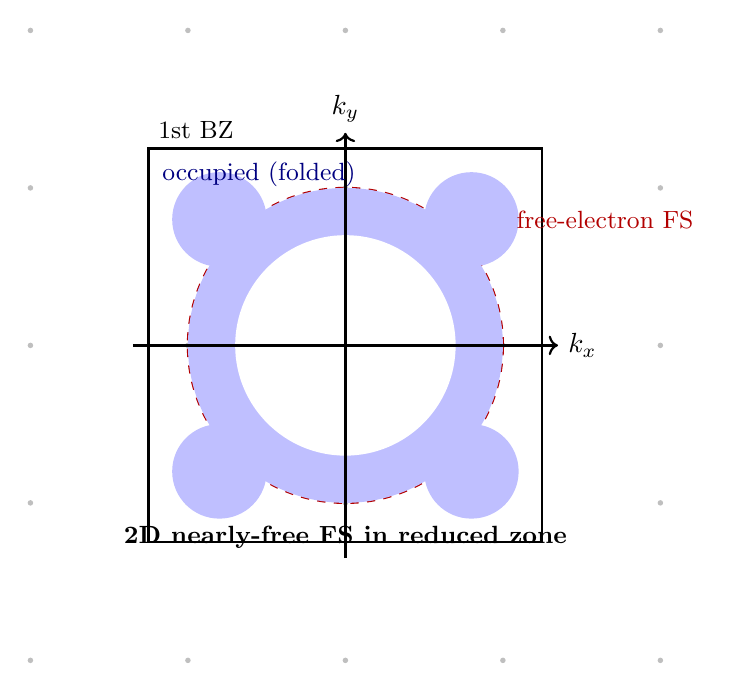
\begin{tikzpicture}
% Square 1st Brillouin zone
\draw[thick, black] (-2.5,-2.5) rectangle (2.5,2.5);
% Reciprocal lattice points
\foreach \x in {-4,-2,...,4}{
    \foreach \y in {-4,-2,...,4}{
        \fill[gray!50] (\x,\y) circle (1.0pt);
    }
}
% BZ center
\node[anchor=south west, font=\small] at (-2.5,2.5) {1st BZ};

% Free-electron circle (radius 2)
\draw[red!70!black, thick, dashed] (0,0) circle (2.0);
% Central occupied
\fill[blue!25] (0,0) circle (1.4);
% Corner pockets (translated)
\fill[blue!25] (1.6,1.6) circle (0.6);
\fill[blue!25] (-1.6,-1.6) circle (0.6);
\fill[blue!25] (1.6,-1.6) circle (0.6);
\fill[blue!25] (-1.6,1.6) circle (0.6);
% Show overlapping piece
\begin{scope}
    \clip (-2.5,-2.5) rectangle (2.5,2.5);
    \fill[blue!25] (0,0) circle (2.0);
    \fill[white] (0,0) circle (1.4);
\end{scope}
% Axes
\draw[->, thick] (-2.7,0) -- (2.7,0) node[right] {$k_x$};
\draw[->, thick] (0,-2.7) -- (0,2.7) node[above] {$k_y$};

\node[anchor=west, font=\small, red!70!black] at (2.05, 1.6) {free-electron FS};
\node[anchor=north west, font=\small, blue!50!black] at (-2.45, 2.45) {occupied (folded)};
\node[anchor=south, font=\small\bfseries] at (0,-2.7) {2D nearly-free FS in reduced zone};
\end{tikzpicture}
\caption{Construction of the Fermi surface in the reduced zone scheme for a 2D square lattice. The free-electron circle (red dashed) is folded into the first Brillouin zone by reciprocal-lattice translations: the central disk becomes the first-band Fermi surface, while the four corner pieces map to four hole pockets (blue) in the second band.}
\label{fig:fs_reduced}
\end{figure}

\paragraph{Electron vs. Hole Pockets:}
\begin{itemize}
    \item If a band is mostly empty with states occupied near the band bottom, the Fermi surface encloses occupied states, forming an \textbf{electron pocket}.
    \item If a band is mostly full with unoccupied states near the band top, the Fermi surface encloses empty states, forming a \textbf{hole pocket}.
\end{itemize}

\subsection{Semiclassical Electron Dynamics in a Magnetic Field}
When a uniform magnetic field $\vb{B} = B\hat{z}$ is applied to a metal, the Lorentz force governs the time evolution of the wavevector:
\begin{equation}
\hbar \frac{d\vb{k}}{dt} = -e\left( \vb{v}\times\vb{B} \right)
\label{eq:lorentz_k_dot}
\end{equation}
This semiclassical equation leads to two fundamental conservation laws:
\begin{enumerate}
    \item \textbf{Energy Conservation}: The rate of work done by the magnetic force is:
    \begin{equation}
    \frac{dE}{dt} = \nabla_{\vb{k}}E \cdot \frac{d\vb{k}}{dt} = (\hbar\vb{v})\cdot\left[ -\frac{e}{\hbar}(\vb{v}\times\vb{B}) \right] = -e\,\vb{v}\cdot(\vb{v}\times\vb{B}) \equiv 0
    \end{equation}
    The electron energy $E(\vb{k}) = \mathrm{constant}$ is strictly conserved throughout the trajectory.
    \item \textbf{Parallel Wavevector Conservation}: Taking the dot product with $\vb{B}$:
    \begin{equation}
    \hbar \frac{d(\vb{k}\cdot\vb{B})}{dt} = -e(\vb{v}\times\vb{B})\cdot\vb{B} \equiv 0 \implies k_z = \mathrm{constant}
    \end{equation}
\end{enumerate}
\textbf{Geometric Trajectory:} In reciprocal space, electrons traverse closed orbits formed by the \textbf{intersection of a constant-energy surface $E(\vb{k}) = E_F$ with a plane of constant $k_z$ perpendicular to $\vb{B}$}!

\paragraph{Cyclotron Frequency and Effective Mass:}
The time required for an electron to complete one full revolution around the orbit is the cyclotron period $T_c = 2\pi/\omega_c$. Integrating $dt = \frac{\hbar\, dk_\perp}{e B v_\perp}$:
\begin{equation}
T_c = \oint dt = \frac{\hbar}{e B}\oint \frac{dk_\perp}{v_\perp}
\end{equation}
Recognizing that the area element between two adjacent energy contours in the $k_x k_y$-plane is $dA = dk_\perp dk_\parallel = dk_\perp \left( \frac{dE}{\hbar v_\perp} \right)$:
\begin{equation}
\oint \frac{dk_\perp}{v_\perp} = \hbar \frac{\partial}{\partial E}\oint dk_\perp dk_\parallel = \hbar \frac{\partial A(E, k_z)}{\partial E}
\end{equation}
Therefore:
\begin{equation}
T_c = \frac{\hbar^2}{e B}\frac{\partial A}{\partial E} \implies \omega_c = \frac{2\pi}{T_c} = \frac{2\pi e B}{\hbar^2 \left(\frac{\partial A}{\partial E}\right)}
\end{equation}
We define the \textbf{cyclotron effective mass} $m_c$ as:
\begin{equation}
\boxed{m_c \equiv \frac{\hbar^2}{2\pi}\left.\frac{\partial A(E, k_z)}{\partial E}\right|_{E=E_F}} \iff \omega_c = \frac{e B}{m_c}
\label{eq:cyclotron_mass_def}
\end{equation}
For a free-electron circle $A(E) = \pi k^2 = \pi \frac{2m_e E}{\hbar^2} \implies \frac{\partial A}{\partial E} = \frac{2\pi m_e}{\hbar^2}$, which recovers $m_c = m_e$.

\subsection{Landau Level Quantization}
In a quantum mechanical treatment, a perpendicular magnetic field $\vb{B} = B\hat{z}$ breaks the continuous $k_x k_y$ continuum into discrete, highly degenerate harmonic oscillator levels known as \textbf{Landau levels}:
\begin{equation}
E_n(k_z) = \left(n + \frac{1}{2}\right)\hbar\omega_c + \frac{\hbar^2 k_z^2}{2m^*}
\label{eq:landau_levels}
\end{equation}
In reciprocal space, the allowed electronic states condense onto a family of concentric, coaxial \textbf{Landau cylinders} (or Landau tubes) aligned along the $k_z$-axis. 

The $k$-space cross-sectional area enclosed by the $n$-th Landau cylinder is given by the Bohr--Sommerfeld semiclassical \textbf{Onsager relation}:
\begin{equation}
\boxed{A_n = \frac{2\pi e B}{\hbar}\left(n + \frac{1}{2}\right)}
\label{eq:onsager_relation}
\end{equation}
The area spacing between adjacent concentric cylinders in $k$-space is:
\begin{equation}
\Delta A = A_{n+1} - A_n = \frac{2\pi e B}{\hbar}
\label{eq:landau_area_spacing}
\end{equation}
Notice that as the magnetic field $B$ increases, the cylinders expand in radius, and their area spacing $\Delta A \propto B$ increases proportionally!

\begin{figure}[h]
\centering
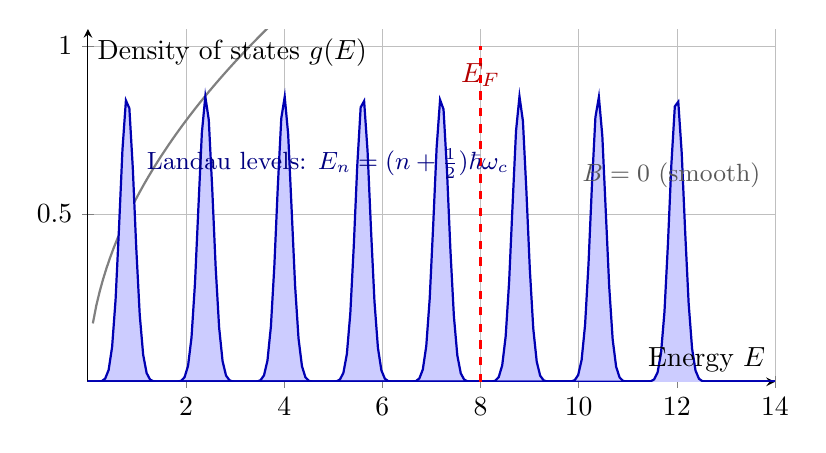
\begin{tikzpicture}
\begin{axis}[
    width=0.85\textwidth,
    height=0.5\textwidth,
    xlabel={Energy $E$},
    ylabel={Density of states $g(E)$},
    xmin=0, xmax=14,
    ymin=0, ymax=1.05,
    grid=both,
    grid style={line width=.1pt, draw=gray!20},
    major grid style={line width=.2pt,draw=gray!50},
    axis lines=middle,
    samples=200,
]
% Smooth free-electron DOS as baseline
\addplot[gray, thick, domain=0.1:14] {0.55*sqrt(x)};

% Landau levels as narrow Gaussians
\foreach \n in {0,1,2,3,4,5,6,7}{
    \pgfmathsetmacro{\xpos}{\n*1.6+0.8}
    \addplot[blue!70!black, thick, fill=blue!20, domain=0:14, samples=200]
        {0.85*exp(-((x-\xpos)^2)/0.045)};
}

% Fermi level
\addplot[red, dashed, thick] coordinates {(8.0, 0) (8.0, 1.0)};
\node[anchor=south, red!70!black, font=\bfseries] at (axis cs:8.0, 0.85) {$E_F$};

% Label one LL
\node[anchor=west, font=\small, blue!50!black] at (axis cs:1.0, 0.65) {Landau levels: $E_n=(n+\tfrac12)\hbar\omega_c$};

% B = 0 baseline label
\node[anchor=south east, font=\small, gray!70!black] at (axis cs:13.9, 0.55) {$B=0$ (smooth)};
\end{axis}
\end{tikzpicture}
\caption{Landau levels in a magnetic field: the 3D free-electron $g(E)\propto\sqrt{E}$ (gray) splits into equally spaced, highly degenerate Landau levels at $E_n=(n+\tfrac12)\hbar\omega_c$ (blue). As $B$ changes, these peaks sweep through $E_F$, causing the oscillatory density of states at the Fermi level that drives the de Haas--van Alphen signal.}
\label{fig:landau}
\end{figure}

\subsection{The de Haas--van Alphen (dHvA) Effect}
As the magnetic field $B$ is continuously increased, the Landau cylinders expand outwards through the fixed Fermi surface. 

Whenever the outermost occupied Landau cylinder expands to touch the extremal cross-section of the Fermi surface and pops through it into the unoccupied region above $E_F$, all the electrons on that cylinder suddenly depopulate, dropping into lower Landau levels. This sudden, periodic depopulation causes the total thermodynamic free energy $F(B)$, magnetization $M(B)$, and magnetic susceptibility $\chi(B)$ to oscillate as a function of the magnetic field!

This celebrated quantum phenomenon is known as the \textbf{de Haas--van Alphen (dHvA) effect} (discovered in 1930 by Wander Johannes de Haas and Pieter M.~van Alphen).

\begin{figure}[h]
\centering
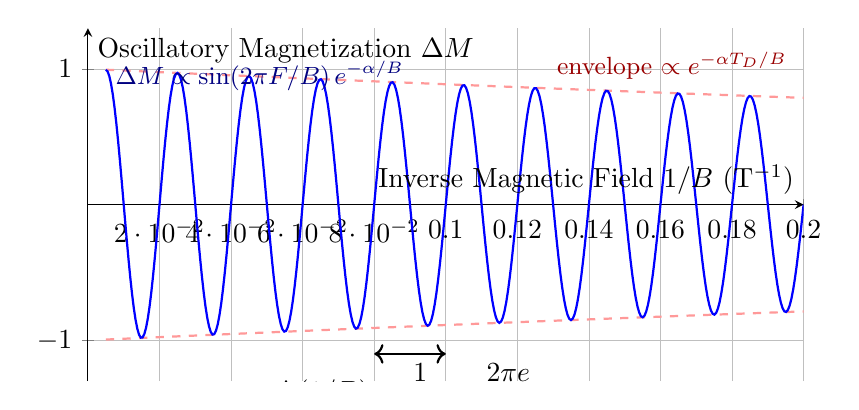
\begin{tikzpicture}
\begin{axis}[
    width=0.88\textwidth,
    height=0.5\textwidth,
    xlabel={Inverse Magnetic Field $1/B$ (T$^{-1}$)},
    ylabel={Oscillatory Magnetization $\Delta M$},
    xmin=0, xmax=0.20,
    ymin=-1.3, ymax=1.3,
    grid=both,
    grid style={line width=.1pt, draw=gray!20},
    major grid style={line width=.2pt,draw=gray!50},
    axis lines=middle,
    samples=400,
]
% Envelope
\addplot[red!40, thick, dashed, domain=0.005:0.2] {exp(-1.2*x)};
\addplot[red!40, thick, dashed, domain=0.005:0.2] {-exp(-1.2*x)};
\node[anchor=south east, red!60!black, font=\small] at (axis cs:0.198, 0.85) {envelope $\propto e^{-\alpha T_D/B}$};

% dHvA oscillation - period 0.02 -> 10 oscillations in [0.005, 0.2]
\addplot[blue, thick, domain=0.005:0.2] {sin(deg(100*pi*x)) * exp(-1.2*x)};
\node[anchor=west, font=\small, blue!50!black] at (axis cs:0.005, 0.95) {$\Delta M\propto\sin(2\pi F/B)\,e^{-\alpha/B}$};

% Period annotation - place at the bottom under two successive peaks
\addplot[black, <->, thick] coordinates {(0.080, -1.10) (0.100, -1.10)};
\node[anchor=north, font=\bfseries] at (axis cs:0.090, -1.10) {$\Delta(1/B)=\dfrac{1}{F}=\dfrac{2\pi e}{\hbar A_{\rm ext}}$};

\end{axis}
\end{tikzpicture}
\caption{Schematic of the de Haas--van Alphen effect, showing oscillations in magnetization periodic in $1/B$. The period is inversely proportional to the extremal cross-sectional area $A_{\rm ext}$ of the Fermi surface. The Dingle factor $e^{-\alpha T_D/B}$ encodes impurity scattering and finite temperature, damping the oscillations at small $B$ (large $1/B$).}
\label{fig:dhva}
\end{figure}

\paragraph{Periodicity in Inverse Field $1/B$:}
A Landau level depopulates whenever its cross-sectional area matches the \textbf{extremal cross-sectional area} $A_{\mathrm{ext}}$ of the Fermi surface:
\begin{equation}
A_{\mathrm{ext}} = \frac{2\pi e B_n}{\hbar}\left(n + \gamma\right) \implies \frac{1}{B_n} = \frac{2\pi e}{\hbar A_{\mathrm{ext}}}(n + \gamma)
\end{equation}
The condition between consecutive oscillation peaks ($n \to n+1$) reveals that dHvA oscillations are strictly \textbf{periodic in inverse magnetic field} $1/B$:
\begin{equation}
\boxed{\Delta\left(\frac{1}{B}\right) = \frac{2\pi e}{\hbar A_{\mathrm{ext}}} = \frac{1}{F}}
\label{eq:dhva_period}
\end{equation}
where $F$ is the \textbf{dHvA oscillation frequency} (measured in Tesla):
\begin{equation}
\boxed{F = \frac{\hbar}{2\pi e}A_{\mathrm{ext}}}
\label{eq:dhva_frequency}
\end{equation}

\begin{takeawaybox}{Why Quantum Oscillations Measure Extremal Cross-Sections}
In three dimensions, the total magnetization involves an integral over all cross-sections along the $k_z$-axis: $M \sim \int dk_z \sin\left(\frac{\hbar A(k_z)}{eB}\right)$. 

For general values of $k_z$, the phase oscillates rapidly, and the contributions from neighboring slices destructively interfere to zero. By the \textbf{principle of stationary phase}, constructive interference occurs exclusively at slices where the cross-sectional area is stationary with respect to $k_z$:
\[
\frac{\partial A(k_z)}{\partial k_z} = 0
\]
These stationary points are precisely the \textbf{extremal cross-sections} (maximal ``belly'' orbits or minimal ``neck'' orbits). Therefore, measuring the dHvA frequency $F$ provides a direct, sub-percent caliper measurement of the extremal cross-sectional dimensions of the Fermi surface!
\end{takeawaybox}

\begin{pitfallbox}{Thermal Washing-Out of Quantum Oscillations}
To observe de Haas--van Alphen oscillations experimentally, two strict physical conditions must be satisfied:
\begin{enumerate}
    \item \textbf{Low Temperature Criterion}: $k_B T \ll \hbar\omega_c$. If the thermal smearing window $k_B T$ is comparable to the Landau level spacing $\hbar\omega_c$, electrons are thermally blurred across multiple levels, completely damping the oscillations. For $B \approx 10\ \mathrm{T}$, $\hbar\omega_c \approx 1\ \mathrm{meV} \sim 10\ \mathrm{K}$, necessitating cryogenic liquid helium temperatures ($T \le 4.2\ \mathrm{K}$).
    \item \textbf{High Purity Criterion}: $\omega_c \tau \gg 1$. Electrons must complete at least one full cyclotron orbit around the Fermi surface before being scattered by impurities ($\tau > T_c$). This requires ultra-high-purity single crystals ($\mathrm{RRR} > 1000$).
\end{enumerate}
\end{pitfallbox}

\vspace{0.4cm}

% -------------------------------------------------------------------------
% SOLVED EXAMPLES FOR CHAPTER 10
% -------------------------------------------------------------------------
\begin{examplebox}{Extremal Area of Copper from dHvA Oscillations}{ex:copper_dhva}
\textbf{Problem Statement:}
In a de Haas--van Alphen experiment on a high-purity single crystal of copper with magnetic field aligned along the $[111]$ crystallographic direction, magnetization oscillations are observed with an inverse field period:
\[
\Delta\left(\frac{1}{B}\right) = 2.18 \times 10^{-5}\ \mathrm{T}^{-1}
\]
Calculate:
\begin{enumerate}[label=(\alph*)]
    \item The extremal cross-sectional area $A_{\mathrm{ext}}$ of the copper Fermi surface in $\mathrm{m}^{-2}$ and in $\text{\AA}^{-2}$.
    \item The fundamental dHvA frequency $F$ in Tesla.
    \item Assuming a spherical Fermi surface, deduce the effective Fermi wavevector $k_F$ and the corresponding Fermi energy $E_F$ in eV.
\end{enumerate}

\vspace{0.2cm}\hrule\vspace{0.2cm}
\textbf{Step-by-Step Solution:}

\textbf{(a) Extremal cross-sectional area $A_{\mathrm{ext}}$:}
From equation~\eqref{eq:dhva_period}:
\begin{align*}
A_{\mathrm{ext}} &= \frac{2\pi e}{\hbar \Delta(1/B)} = \frac{2\pi(1.6022 \times 10^{-19}\ \mathrm{C})}{(1.0546 \times 10^{-34}\ \mathrm{J\cdot s})(2.18 \times 10^{-5}\ \mathrm{T^{-1}})} \\
&= \frac{1.0067 \times 10^{-18}}{2.299 \times 10^{-39}} \approx \mathbf{4.38 \times 10^{20}\ \mathrm{m^{-2}}} = \mathbf{4.38\ \text{\AA}^{-2}}
\end{align*}

\textbf{(b) dHvA frequency $F$:}
\[
F = \frac{1}{\Delta(1/B)} = \frac{1}{2.18 \times 10^{-5}\ \mathrm{T^{-1}}} \approx \mathbf{45{,}870\ \mathrm{T}} \approx 4.59 \times 10^4\ \mathrm{T}
\]

\textbf{(c) Effective Fermi wavevector and Fermi energy:}
For a circular cross-section, $A_{\mathrm{ext}} = \pi k_F^2$:
\[
k_F = \sqrt{\frac{A_{\mathrm{ext}}}{\pi}} = \sqrt{\frac{4.38 \times 10^{20}\ \mathrm{m^{-2}}}{\pi}} = \sqrt{1.394 \times 10^{20}} \approx \mathbf{1.18 \times 10^{10}\ \mathrm{m^{-1}}} = 1.18\ \text{\AA}^{-1}
\]
The corresponding Fermi energy is:
\begin{align*}
E_F &= \frac{\hbar^2 k_F^2}{2m_e} = \frac{(1.0546 \times 10^{-34}\ \mathrm{J\cdot s})^2 (1.181 \times 10^{10}\ \mathrm{m^{-1}})^2}{2(9.109 \times 10^{-31}\ \mathrm{kg})} \\
&= \frac{(1.112 \times 10^{-68})(1.394 \times 10^{20})}{1.822 \times 10^{-30}} \approx 8.51 \times 10^{-19}\ \mathrm{J} = \frac{8.51 \times 10^{-19}\ \mathrm{J}}{1.6022 \times 10^{-19}\ \mathrm{J/eV}} \approx \mathbf{5.31\ \mathrm{eV}}
\end{align*}
(The slight deviation from the belly value $E_F \approx 7.0\ \mathrm{eV}$ reflects the fact that the $[111]$ orbit in copper measures the narrower neck that contacts the Brillouin zone face!).
\end{examplebox}

\vspace{0.4cm}

\begin{examplebox}{Extraction of Fermi Parameters from dHvA Frequency}{ex:dhva_freq_params}
\textbf{Problem Statement:}
A metal displays a dominant dHvA oscillation frequency of $F = 5000\ \mathrm{T}$.
\begin{enumerate}[label=(\alph*)]
    \item Calculate the extremal area $A_{\mathrm{ext}}$ of the Fermi surface in $\mathrm{m}^{-2}$.
    \item Assuming an isotropic spherical Fermi surface, determine the Fermi wavevector $k_F$, the electron density $n$, and the Fermi energy $E_F$ in eV.
\end{enumerate}

\vspace{0.2cm}\hrule\vspace{0.2cm}
\textbf{Step-by-Step Solution:}

\textbf{(a) Extremal cross-sectional area:}
From equation~\eqref{eq:dhva_frequency}:
\begin{align*}
A_{\mathrm{ext}} &= \frac{2\pi e}{\hbar}F = \frac{2\pi(1.6022 \times 10^{-19}\ \mathrm{C})}{1.0546 \times 10^{-34}\ \mathrm{J\cdot s}}(5000\ \mathrm{T}) \\
&= (9.546 \times 10^{15}\ \mathrm{m^{-2}T^{-1}})(5000\ \mathrm{T}) \approx \mathbf{4.77 \times 10^{19}\ \mathrm{m^{-2}}} = 0.477\ \text{\AA}^{-2}
\end{align*}

\textbf{(b) Fermi wavevector, electron density, and Fermi energy:}
For a sphere, $A_{\mathrm{ext}} = \pi k_F^2$:
\[
k_F = \sqrt{\frac{A_{\mathrm{ext}}}{\pi}} = \sqrt{\frac{4.773 \times 10^{19}\ \mathrm{m^{-2}}}{\pi}} \approx \mathbf{3.90 \times 10^9\ \mathrm{m^{-1}}} = 0.390\ \text{\AA}^{-1}
\]
The conduction electron density is:
\[
n = \frac{k_F^3}{3\pi^2} = \frac{(3.898 \times 10^9\ \mathrm{m^{-1}})^3}{3\pi^2} = \frac{5.923 \times 10^{28}}{29.609} \approx \mathbf{2.00 \times 10^{27}\ \mathrm{m^{-3}}}
\]
The Fermi energy is:
\begin{align*}
E_F &= \frac{\hbar^2 k_F^2}{2m_e} = \frac{(1.0546 \times 10^{-34})^2 (3.898 \times 10^9)^2}{2(9.109 \times 10^{-31})} = \frac{1.690 \times 10^{-49}}{1.822 \times 10^{-30}} \approx 9.276 \times 10^{-20}\ \mathrm{J} \\
E_F &= \frac{9.276 \times 10^{-20}\ \mathrm{J}}{1.6022 \times 10^{-19}\ \mathrm{J/eV}} \approx \mathbf{0.579\ \mathrm{eV}} \approx \mathbf{0.58\ \mathrm{eV}}
\end{align*}
\end{examplebox}

\clearpage


% =========================================================================
% CHAPTER 11: COMPREHENSIVE SOLVED PROBLEMS & TUTORIAL SOLUTIONS
% =========================================================================
\section{Comprehensive Solved Problems and Tutorial Solutions}
\label{sec:capstone_problems}

\noindent This chapter provides complete, multi-part, step-by-step solutions to advanced tutorial problems that synthesize thermodynamics, transport, band theory, and quantum oscillations across Module 3.

\vspace{0.3cm}

\subsection{Problem 11.1: Complete Electronic Ground State of Monovalent Noble Metals}
\textbf{Problem Statement:}
Silver (Ag) crystallizes in a face-centered cubic (FCC) structure with a conventional lattice parameter $a = 4.09\ \text{\AA}$. Silver has atomic mass $A = 107.87\ \mathrm{g/mol}$, mass density $\rho_m = 10.50 \times 10^3\ \mathrm{kg/m^3}$, and each atom contributes exactly one valence electron ($Z_v = 1$).
\begin{enumerate}[label=(\alph*)]
    \item Calculate the conduction electron density $n$ independently via: (i) the crystallographic FCC unit cell volume, and (ii) macroscopic mass density. Compare the two results.
    \item Determine the Fermi wavevector $k_F$, the radius of the Fermi sphere, and verify that the Fermi sphere does not intersect the first Brillouin zone boundary along the $[100]$ direction ($k_{\mathrm{BZ}} = 2\pi/a$).
    \item Calculate the Fermi energy $E_F$ (in eV), the Fermi velocity $v_F$, and the Fermi temperature $T_F$.
    \item Compute the zero-point ground-state internal energy $U_0$ and the degeneracy pressure $P_0$ exerted by the conduction electrons.
\end{enumerate}

\vspace{0.2cm}\hrule\vspace{0.2cm}
\textbf{Step-by-Step Solution:}

\textbf{(a) Conduction electron concentration $n$:}
\begin{enumerate}[label=(\roman*)]
    \item \emph{From crystallographic unit cell}: In an FCC Bravais lattice, there are $4$ atoms per cubic unit cell ($8 \times \frac{1}{8} + 6 \times \frac{1}{2} = 4$). Since each atom donates $1$ electron:
    \[
    n = \frac{4 Z_v}{a^3} = \frac{4 \times 1}{(4.09 \times 10^{-10}\ \mathrm{m})^3} = \frac{4}{6.842 \times 10^{-29}\ \mathrm{m^3}} \approx \mathbf{5.846 \times 10^{28}\ \mathrm{m^{-3}}}
    \]
    \item \emph{From macroscopic mass density}:
    \[
    n = \frac{Z_v N_A \rho_m}{A} = \frac{(1)(6.0221 \times 10^{23}\ \mathrm{mol^{-1}})(10.50 \times 10^3\ \mathrm{kg/m^3})}{107.87 \times 10^{-3}\ \mathrm{kg/mol}} = \frac{6.323 \times 10^{27}}{0.10787} \approx \mathbf{5.862 \times 10^{28}\ \mathrm{m^{-3}}}
    \]
    The two independent methods agree to within $0.27\%$! We adopt $n = 5.86 \times 10^{28}\ \mathrm{m^{-3}}$.
\end{enumerate}

\textbf{(b) Fermi wavevector and Brillouin zone geometry:}
\[
k_F = (3\pi^2 n)^{1/3} = \left[ 3\pi^2 (5.86 \times 10^{28}\ \mathrm{m^{-3}}) \right]^{1/3} = (1.735 \times 10^{30})^{1/3} \approx \mathbf{1.202 \times 10^{10}\ \mathrm{m^{-1}}} = 1.202\ \text{\AA}^{-1}
\]
For an FCC lattice, the shortest distance from the zone center $\Gamma$ to the square face of the first Brillouin zone ($X$-point along $[100]$) is:
\[
k_X = \frac{2\pi}{a} = \frac{2\pi}{4.09 \times 10^{-10}\ \mathrm{m}} \approx \mathbf{1.536 \times 10^{10}\ \mathrm{m^{-1}}} = 1.536\ \text{\AA}^{-1}
\]
Comparing the radii:
\[
\frac{k_F}{k_X} = \frac{1.202}{1.536} \approx 0.783 < 1
\]
The Fermi sphere lies well inside the first Brillouin zone along $[100]$. (Along $[111]$, the distance to the hexagonal face is $k_L = \sqrt{3}\pi/a \approx 1.330\ \text{\AA}^{-1}$, where the neck of the silver Fermi surface pulls out and contacts the zone face).

\textbf{(c) Fermi energy, velocity, and temperature:}
\begin{align*}
E_F &= \frac{\hbar^2 k_F^2}{2m_e} = \frac{(1.0546 \times 10^{-34}\ \mathrm{J\cdot s})^2 (1.202 \times 10^{10}\ \mathrm{m^{-1}})^2}{2(9.1094 \times 10^{-31}\ \mathrm{kg})} \approx 8.816 \times 10^{-19}\ \mathrm{J} = \mathbf{5.50\ \mathrm{eV}} \\
v_F &= \frac{\hbar k_F}{m_e} = \frac{(1.0546 \times 10^{-34})(1.202 \times 10^{10})}{9.1094 \times 10^{-31}} \approx \mathbf{1.39 \times 10^6\ \mathrm{m/s}} \\
T_F &= \frac{E_F}{k_B} = \frac{8.816 \times 10^{-19}\ \mathrm{J}}{1.3807 \times 10^{-23}\ \mathrm{J/K}} \approx \mathbf{6.38 \times 10^4\ \mathrm{K}} \approx 63{,}800\ \mathrm{K}
\end{align*}

\textbf{(d) Ground-state energy density and degeneracy pressure:}
\begin{align*}
u_0 &= \frac{U_0}{V} = \frac{3}{5}n E_F = \frac{3}{5}(5.86 \times 10^{28}\ \mathrm{m^{-3}})(8.816 \times 10^{-19}\ \mathrm{J}) \approx \mathbf{3.10 \times 10^{10}\ \mathrm{J/m^3}} \\
P_0 &= \frac{2}{3}u_0 = \frac{2}{3}(3.10 \times 10^{10}\ \mathrm{J/m^3}) \approx \mathbf{2.07 \times 10^{10}\ \mathrm{Pa}} \approx \mathbf{204{,}000\ \mathrm{atm}}
\end{align*}

\vspace{0.4cm}

\subsection{Problem 11.2: Quantum Degeneracy Pressure and White Dwarf Collapse}
\textbf{Problem Statement:}
In a white dwarf star, matter is completely ionized into helium or carbon/oxygen nuclei and a dense, degenerate electron gas. Consider a white dwarf of mass $M$ and radius $R$ with uniform mass density $\rho_m = \frac{M}{\frac{4}{3}\pi R^3}$. Let the number of nucleons per electron be $\mu_e = 2$ (e.g., $^{12}\mathrm{C}$ has $6$ protons, $6$ neutrons, and $6$ electrons, so $\mu_e = 12/6 = 2$).
\begin{enumerate}[label=(\alph*)]
    \item Express the electron number density $n$ in terms of mass density $\rho_m$ and proton mass $m_p$.
    \item Derive the non-relativistic degeneracy pressure $P_{\mathrm{NR}}$ as a function of $\rho_m$.
    \item In the ultra-relativistic limit ($E \approx p c \gg m_e c^2$), show that the degeneracy pressure scales as $P_{\mathrm{UR}} \propto \rho_m^{4/3}$.
    \item Explain physically why this transition from $P \propto \rho^{5/3}$ to $P \propto \rho^{4/3}$ leads directly to the Chandrasekhar mass limit ($M_{\mathrm{Ch}} \approx 1.44 M_\odot$).
\end{enumerate}

\vspace{0.2cm}\hrule\vspace{0.2cm}
\textbf{Step-by-Step Solution:}

\textbf{(a) Electron concentration $n$:}
The mass of the star is overwhelmingly carried by the nucleons: $M \approx N_{\mathrm{nucleons}} m_p$. Because there is $1$ electron for every $\mu_e$ nucleons:
\[
n = \frac{N_e}{V} = \frac{N_{\mathrm{nucleons}}}{\mu_e V} = \frac{\rho_m}{\mu_e m_p}
\]

\textbf{(b) Non-relativistic degeneracy pressure:}
From equation~\eqref{eq:fermi_pressure}, $P_0 = \frac{2}{5}n E_F = \frac{\hbar^2}{5m_e}(3\pi^2)^{2/3} n^{5/3}$. Substituting $n = \rho_m / (\mu_e m_p)$:
\[
P_{\mathrm{NR}} = \frac{\hbar^2}{5m_e}(3\pi^2)^{2/3} \left( \frac{\rho_m}{\mu_e m_p} \right)^{5/3} \propto \rho_m^{5/3} \propto \left(\frac{M}{R^3}\right)^{5/3} = \frac{M^{5/3}}{R^5}
\]

\textbf{(c) Ultra-relativistic degeneracy pressure:}
When density becomes extreme ($\rho_m \gtrsim 10^9\ \mathrm{kg/m^3}$), $p_F \gg m_e c$, and electron dispersion becomes ultra-relativistic: $E(p) \approx p c = \hbar c k$.
The total ground-state internal energy is:
\[
U_{\mathrm{UR}} = 2 \sum_{|\vb{k}| \le k_F} \hbar c k = 2 \frac{V}{(2\pi)^3}\int_0^{k_F} (\hbar c k)(4\pi k^2 dk) = \frac{V \hbar c}{\pi^2}\int_0^{k_F} k^3 dk = \frac{V \hbar c}{4\pi^2}k_F^4
\]
Since $k_F = (3\pi^2 n)^{1/3}$:
\[
U_{\mathrm{UR}} = \frac{V \hbar c}{4\pi^2}(3\pi^2 n)^{4/3} = \frac{3}{4}\hbar c (3\pi^2)^{1/3} n^{4/3} V = \frac{3}{4} N E_F
\]
The relativistic degeneracy pressure is:
\[
P_{\mathrm{UR}} = -\frac{\partial U_{\mathrm{UR}}}{\partial V} = \frac{1}{3}\frac{U_{\mathrm{UR}}}{V} = \frac{1}{4}\hbar c (3\pi^2)^{1/3} n^{4/3}
\]
Substituting $n = \rho_m / (\mu_e m_p)$:
\[
\boxed{P_{\mathrm{UR}} = \frac{\hbar c}{4}(3\pi^2)^{1/3} \left( \frac{\rho_m}{\mu_e m_p} \right)^{4/3} \propto \rho_m^{4/3} \propto \frac{M^{4/3}}{R^4}}
\]

\textbf{(d) Physical origin of the Chandrasekhar Limit:}
Hydrostatic equilibrium requires the internal pressure gradient force to balance gravitational inward pull:
\[
F_{\mathrm{pressure}} \sim P R^2, \quad F_{\mathrm{gravity}} \sim \frac{G M^2}{R^2}
\]
\begin{itemize}
    \item In the non-relativistic regime:
    \[
    P_{\mathrm{NR}} R^2 \sim \frac{M^{5/3}}{R^5} R^2 = \frac{M^{5/3}}{R^3} \sim \frac{G M^2}{R^2} \implies R \propto M^{-1/3}
    \]
    As mass increases, the star contracts to a smaller, stable radius $R$.
    \item In the ultra-relativistic regime:
    \[
    P_{\mathrm{UR}} R^2 \sim \frac{M^{4/3}}{R^4} R^2 = \frac{M^{4/3}}{R^2} \sim \frac{G M^2}{R^2}
    \]
    The radius $R$ cancels out completely from both sides! Gravitational force and degeneracy pressure exhibit the \textbf{identical $1/R^2$ scaling}.
\end{itemize}
Equating the two yields an absolute critical maximum mass:
\[
M_{\mathrm{Ch}} \approx \frac{\omega_3^0}{m_p^2}\left(\frac{\hbar c}{G}\right)^{3/2} \approx 1.44 M_\odot
\]
If a stellar remnant exceeds $1.44 M_\odot$, relativistic electron degeneracy pressure is mathematically incapable of halting gravitational contraction; the star must collapse into a neutron star or black hole.

\vspace{0.4cm}

\subsection{Problem 11.3: Determination of Fermi Energy from Specific Heat}
\textbf{Problem Statement:}
Low-temperature heat capacity measurements on an unknown monovalent metallic element yield an electronic coefficient $C_{el} = 2.50 \times 10^{-4} T\ \mathrm{J\,mol^{-1}\,K^{-1}}$.
\begin{enumerate}[label=(\alph*)]
    \item Calculate the experimental Fermi energy $E_F$ in Joules and in electron-volts.
    \item Determine the density of states at the Fermi energy per mole, $g(E_F)$.
    \item Compute the theoretical Fermi wavevector $k_F$ and the conduction electron concentration $n$.
\end{enumerate}

\vspace{0.2cm}\hrule\vspace{0.2cm}
\textbf{Step-by-Step Solution:}

\textbf{(a) Fermi energy $E_F$:}
The experimental Sommerfeld coefficient is $\gamma = 2.50 \times 10^{-4}\ \mathrm{J\,mol^{-1}\,K^{-2}}$.
Using equation~\eqref{eq:sommerfeld_gamma} for one mole:
\[
\gamma = \frac{\pi^2 R k_B}{2 E_F} \implies E_F = \frac{\pi^2 R k_B}{2\gamma}
\]
Substituting $R = 8.3145\ \mathrm{J/(mol\cdot K)}$ and $k_B = 1.3807 \times 10^{-23}\ \mathrm{J/K}$:
\begin{align*}
E_F &= \frac{\pi^2 (8.3145)(1.3807 \times 10^{-23})}{2(2.50 \times 10^{-4})} = \frac{1.133 \times 10^{-21}}{5.00 \times 10^{-4}} \approx \mathbf{2.266 \times 10^{-18}\ \mathrm{J}} \\
E_F &= \frac{2.266 \times 10^{-18}\ \mathrm{J}}{1.6022 \times 10^{-19}\ \mathrm{J/eV}} \approx \mathbf{14.14\ \mathrm{eV}}
\end{align*}

\textbf{(b) Density of states at $E_F$:}
From equation~\eqref{eq:sommerfeld_gamma}, $\gamma = \frac{\pi^2}{3}k_B^2 g(E_F)$:
\begin{align*}
g(E_F) &= \frac{3\gamma}{\pi^2 k_B^2} = \frac{3(2.50 \times 10^{-4}\ \mathrm{J\,mol^{-1}\,K^{-2}})}{\pi^2 (1.3807 \times 10^{-23}\ \mathrm{J/K})^2} = \frac{7.50 \times 10^{-4}}{\pi^2 (1.906 \times 10^{-45})} \\
&\approx \mathbf{3.99 \times 10^{41}\ \mathrm{states\,J^{-1}\,mol^{-1}}} = \mathbf{6.39 \times 10^{22}\ \mathrm{states\,eV^{-1}\,mol^{-1}}}
\end{align*}

\textbf{(c) Fermi wavevector and electron density:}
From $E_F = \frac{\hbar^2 k_F^2}{2m_e}$:
\begin{align*}
k_F &= \sqrt{\frac{2m_e E_F}{\hbar^2}} = \sqrt{\frac{2(9.1094 \times 10^{-31}\ \mathrm{kg})(2.266 \times 10^{-18}\ \mathrm{J})}{(1.0546 \times 10^{-34}\ \mathrm{J\cdot s})^2}} = \sqrt{\frac{4.128 \times 10^{-48}}{1.112 \times 10^{-68}}} \\
&= \sqrt{3.712 \times 10^{20}} \approx \mathbf{1.927 \times 10^{10}\ \mathrm{m^{-1}}} = 1.927\ \text{\AA}^{-1}
\end{align*}
The electron concentration is:
\[
n = \frac{k_F^3}{3\pi^2} = \frac{(1.927 \times 10^{10}\ \mathrm{m^{-1}})^3}{3\pi^2} = \frac{7.155 \times 10^{30}}{29.609} \approx \mathbf{2.42 \times 10^{29}\ \mathrm{m^{-3}}}
\]

\vspace{0.4cm}

\subsection{Problem 11.4: Band Gaps in a 1D Superlattice Potential}
\textbf{Problem Statement:}
An artificial 1D semiconductor superlattice of period $a = 5.00\ \text{\AA}$ has a crystal potential represented by $V(x) = V_0 \cos(2\pi x/a)$ with $V_0 = 1.00\ \mathrm{eV}$.
\begin{enumerate}[label=(\alph*)]
    \item Determine the non-zero Fourier coefficients $V_G$.
    \item Calculate the energy band gap $\Delta E_1$ at the first Brillouin zone boundary $k = \pi/a$.
    \item Does this potential open an energy gap at the second zone boundary $k = 2\pi/a$ to first order in perturbation theory? What higher-order process opens a gap at $k = 2\pi/a$?
\end{enumerate}

\vspace{0.2cm}\hrule\vspace{0.2cm}
\textbf{Step-by-Step Solution:}

\textbf{(a) Fourier coefficients:}
Expanding $V(x) = \frac{V_0}{2}e^{i(2\pi/a)x} + \frac{V_0}{2}e^{-i(2\pi/a)x}$:
\[
V_{\pm 2\pi/a} = \frac{V_0}{2} = \frac{1.00\ \mathrm{eV}}{2} = \mathbf{0.50\ \mathrm{eV}}
\]
All other Fourier components $V_G$ for $G \neq \pm 2\pi/a$ are identically zero.

\textbf{(b) Band gap at the first zone boundary ($k = \pi/a$):}
At $k = \pi/a$, the state $|k\rangle = |\pi/a\rangle$ is coupled to $|k-G\rangle = |\pi/a - 2\pi/a\rangle = |-\pi/a\rangle$ by $G = 2\pi/a$.
The band gap is:
\[
\Delta E_1 = 2|V_{2\pi/a}| = 2(0.50\ \mathrm{eV}) = \mathbf{1.00\ \mathrm{eV}}
\]

\textbf{(c) Second zone boundary ($k = 2\pi/a$):}
At the second zone boundary $k = 2\pi/a$, coupling to $|k'\rangle = |-2\pi/a\rangle$ requires a reciprocal lattice vector $G' = 4\pi/a$.
Because $V(x)$ is a pure cosine, the Fourier amplitude $V_{4\pi/a} = 0$. 
Therefore, to \textbf{first order} in perturbation theory, the band gap at $k = 2\pi/a$ vanishes: $\Delta E_2^{(1)} = 2|V_{4\pi/a}| = \mathbf{0}$.

However, a non-zero band gap is opened to \textbf{second order} via an intermediate virtual state. The state $|2\pi/a\rangle$ couples to $|0\rangle$ via $V_{-2\pi/a}$, which subsequently couples to $|-2\pi/a\rangle$ via $V_{-2\pi/a}$. The second-order effective matrix element is:
\[
V_{\mathrm{eff}}^{(2)} \sim \frac{|V_{2\pi/a}|^2}{E^{(0)}(2\pi/a) - E^{(0)}(0)} \implies \Delta E_2^{(2)} \approx \frac{2|V_{2\pi/a}|^2}{E^{(0)}(2\pi/a)}
\]
This produces a much narrower second-order band gap at $k = 2\pi/a$.

\vspace{0.4cm}

\subsection{Problem 11.5: Multi-Orbit Fermi Surface Reconstruction in Divalent Metals}
\textbf{Problem Statement:}
In a de Haas--van Alphen oscillation experiment on a divalent hexagonal metal, the magnetic field is oriented along the hexagonal $c$-axis. Two distinct oscillation frequencies are observed in the Fourier spectrum of the magnetization:
\[
F_1 = 1200\ \mathrm{T} \quad \text{and} \quad F_2 = 5600\ \mathrm{T}
\]
\begin{enumerate}[label=(\alph*)]
    \item Calculate the extremal cross-sectional areas $A_1$ and $A_2$ of the two orbits in $\mathrm{m}^{-2}$ and in $\text{\AA}^{-2}$.
    \item Explain physically how a single metal can exhibit two distinct dHvA frequencies for the same field orientation.
    \item Assuming both orbits are circular, compute their effective radii in $k$-space ($k_1$ and $k_2$).
\end{enumerate}

\vspace{0.2cm}\hrule\vspace{0.2cm}
\textbf{Step-by-Step Solution:}

\textbf{(a) Extremal cross-sectional areas:}
Using the Onsager frequency relation $A_{\mathrm{ext}} = \frac{2\pi e}{\hbar}F$:
\begin{align*}
A_1 &= \frac{2\pi(1.6022 \times 10^{-19}\ \mathrm{C})}{1.0546 \times 10^{-34}\ \mathrm{J\cdot s}}(1200\ \mathrm{T}) = (9.546 \times 10^{15})(1200) \approx \mathbf{1.146 \times 10^{19}\ \mathrm{m^{-2}}} = \mathbf{0.115\ \text{\AA}^{-2}} \\
A_2 &= (9.546 \times 10^{15})(5600\ \mathrm{T}) \approx \mathbf{5.346 \times 10^{19}\ \mathrm{m^{-2}}} = \mathbf{0.535\ \text{\AA}^{-2}}
\end{align*}

\textbf{(b) Physical origin of multiple frequencies:}
Multiple dHvA frequencies for a single magnetic field orientation arise from two distinct physical mechanisms:
\begin{enumerate}
    \item \textbf{Multiple Extremal Slices of a Single Surface}: A non-spherical Fermi surface (such as a dumbbell or corrugated cylinder) possesses multiple cross-sections where $\partial A/\partial k_z = 0$. For example, a dumbbell has a maximal cross-section (the wide ``belly'') and a minimal cross-section (the narrow ``neck'').
    \item \textbf{Multiple Separate Fermi Surface Sheets}: In a multiband metal (such as a divalent metal with overlapping bands), the Fermi surface consists of multiple disconnected pieces in different Brillouin zones: small hole pockets in one band (yielding small frequency $F_1$) and large electron pockets in another band (yielding large frequency $F_2$).
\end{enumerate}

\textbf{(c) Effective orbital radii:}
Assuming circular cross-sections ($A = \pi k^2$):
\begin{align*}
k_1 &= \sqrt{\frac{A_1}{\pi}} = \sqrt{\frac{1.146 \times 10^{19}}{\pi}} \approx \mathbf{1.91 \times 10^9\ \mathrm{m^{-1}}} = 0.191\ \text{\AA}^{-1} \\
k_2 &= \sqrt{\frac{A_2}{\pi}} = \sqrt{\frac{5.346 \times 10^{19}}{\pi}} \approx \mathbf{4.13 \times 10^9\ \mathrm{m^{-1}}} = 0.413\ \text{\AA}^{-1}
\end{align*}

\clearpage


% =========================================================================
% APPENDIX A: PYTHON DEMONSTRATION SCRIPTS
% =========================================================================
\clearpage
\appendix
\section{Appendix A: Python Demonstration Scripts}
\label{sec:appendix_python}

\noindent\textit{The following standalone Python scripts provide interactive computational implementations of the central theoretical concepts in Module 3. Students are encouraged to execute, modify, and explore these scripts to deepen their physical and numerical intuition.}

\subsection{Fermi Energy Calculator}

\begin{lstlisting}
import numpy as np

# Physical constants
hbar = 1.055e-34   # J s
m_e = 9.11e-31     # kg
eV = 1.602e-19     # J

# Typical electron densities in m^-3
metals = {
    "Cu": 8.5e28,
    "Ag": 5.86e28,
    "Al": 18.1e28,
    "Na": 2.65e28,
    "Fe": 17.0e28,
    "Au": 5.90e28
}

def fermi_energy(n):
    """Return Fermi energy in eV."""
    kF = (3.0 * np.pi**2 * n)**(1.0/3.0)
    EF = hbar**2 * kF**2 / (2.0 * m_e)
    return EF / eV

def fermi_velocity(n):
    """Return Fermi velocity in m/s."""
    kF = (3.0 * np.pi**2 * n)**(1.0/3.0)
    return hbar * kF / m_e

print(f"{'Metal':<6} {'n (1e28/m^3)':<16} {'EF (eV)':<10} {'vF (1e6 m/s)':<15}")
print("-" * 55)

for metal, n in metals.items():
    EF = fermi_energy(n)
    vF = fermi_velocity(n) / 1.0e6
    print(f"{metal:<6} {n/1.0e28:<16.2f} {EF:<10.2f} {vF:<15.2f}")
\end{lstlisting}

\subsection{Fermi--Dirac Distribution Visualization}

\begin{lstlisting}
import numpy as np
import matplotlib.pyplot as plt

def fermi_dirac(E, mu, T):
    """Fermi-Dirac distribution. E and mu in eV, T in K."""
    kB = 8.617e-5  # eV/K
    if T == 0:
        return np.where(E < mu, 1.0, 0.0)
    return 1.0 / (np.exp((E - mu) / (kB * T)) + 1.0)

E = np.linspace(-0.5, 0.5, 1000)
mu = 0.0
T_values = [0, 100, 300, 1000, 3000]

plt.figure(figsize=(7, 4))

for T in T_values:
    f = fermi_dirac(E, mu, T)
    plt.plot(E, f, label=f"T = {T} K")

plt.axvline(0, color="gray", linestyle="--", alpha=0.5)
plt.xlabel("E - EF (eV)")
plt.ylabel("f(E)")
plt.title("Fermi-Dirac Distribution")
plt.legend()
plt.grid(True, alpha=0.3)
plt.tight_layout()
plt.show()
\end{lstlisting}

\subsection{Electronic and Phonon Specific Heat}

\begin{lstlisting}
import numpy as np
import matplotlib.pyplot as plt

# Approximate copper parameters
gamma = 0.695   # mJ/mol/K^2
beta = 0.048    # mJ/mol/K^4

T = np.linspace(0.1, 15, 500)

C_el = gamma * T
C_ph = beta * T**3
C_total = C_el + C_ph

plt.figure(figsize=(7, 4))
plt.plot(T, C_el, label="Electronic, gamma*T")
plt.plot(T, C_ph, label="Phonon, beta*T^3")
plt.plot(T, C_total, "k--", label="Total")

plt.xlabel("T (K)")
plt.ylabel("C_V (mJ/mol/K)")
plt.title("Low-T Specific Heat of Copper")
plt.legend()
plt.grid(True, alpha=0.3)
plt.tight_layout()
plt.show()

# Temperature where electronic and phonon parts are equal
T_eq = np.sqrt(gamma / beta)
print(f"Crossover temperature = {T_eq:.2f} K")
\end{lstlisting}

\subsection{Nearly Free Electron Gap Illustration}

\begin{lstlisting}
import numpy as np
import matplotlib.pyplot as plt

# 1D nearly-free-electron illustration
a = 1.0
G = 2.0 * np.pi / a
VG = 0.3

k = np.linspace(-1.8, 1.8, 2000)
E_free = k**2

# Two-band avoided-crossing model near k = +/- 1 (which is +/- pi/a for a=2)
# Using the exact secular equation solution
E_lower = (k**2 + (k-2)**2)/2 - np.sqrt(((k**2 - (k-2)**2)/2)**2 + VG**2)
E_upper = (k**2 + (k-2)**2)/2 + np.sqrt(((k**2 - (k-2)**2)/2)**2 + VG**2)

plt.figure(figsize=(8, 4.5))
plt.plot(k, E_free, "k--", alpha=0.5, label="Free electron")
plt.plot(k, (k-2)**2, "k--", alpha=0.5)
plt.plot(k, E_lower, "b", linewidth=2, label="Lower band")
plt.plot(k, E_upper, "r", linewidth=2, label="Upper band")

plt.axvline(1, color="gray", linestyle=":")
plt.axvline(-1, color="gray", linestyle=":")

plt.xlabel("k")
plt.ylabel("E (arbitrary units)")
plt.title("Nearly Free Electron Band Gap at Zone Boundary")
plt.legend()
plt.grid(True, alpha=0.3)
plt.tight_layout()
plt.show()
\end{lstlisting}

\subsection{de Haas--van Alphen Oscillation Model}

\begin{lstlisting}
import numpy as np
import matplotlib.pyplot as plt

B = np.linspace(1.0, 20.0, 2000)
F = 50.0       # dHvA frequency factor
T = 1.0        # temperature in K

# Simplified oscillation with damping
invB = 1.0 / B
chi = np.sin(2.0 * np.pi * F * invB) * np.exp(-2.0 * invB)

fig, axes = plt.subplots(1, 2, figsize=(11, 4))

axes[0].plot(B, chi)
axes[0].set_xlabel("B (T)")
axes[0].set_ylabel("Oscillatory susceptibility")
axes[0].set_title("dHvA oscillations vs B")
axes[0].grid(True, alpha=0.3)

axes[1].plot(invB, chi)
axes[1].set_xlabel("1/B (1/T)")
axes[1].set_ylabel("Oscillatory susceptibility")
axes[1].set_title("Periodic in 1/B")
axes[1].grid(True, alpha=0.3)

plt.tight_layout()
plt.show()
\end{lstlisting}

\clearpage

% =========================================================================
% APPENDIX B: MASTER FORMULA REFERENCE TABLE
% =========================================================================
\section{Appendix B: Master Formula Reference Table}
\label{sec:appendix_formulas}

\noindent A comprehensive analytical reference guide summarizing the 26 central formulas across Module 3:

\begin{longtable}{p{0.32\textwidth} p{0.44\textwidth} p{0.18\textwidth}}
\toprule
\textbf{Physical Quantity} & \textbf{Mathematical Formula} & \textbf{Chapter Reference} \\
\midrule
\endfirsthead
\toprule
\textbf{Physical Quantity} & \textbf{Mathematical Formula} & \textbf{Chapter Reference} \\
\midrule
\endhead
\bottomrule
\endfoot

\textbf{Drude DC Conductivity} & $\sigma_0 = \dfrac{n e^2 \tau}{m_e}$ & Chapter~\ref{sec:drude_theory} \\
\textbf{Electron Mobility} & $\mu = \dfrac{|\vb{v}_d|}{E} = \dfrac{e\tau}{m_e}$ & Chapter~\ref{sec:drude_theory} \\
\textbf{AC Optical Conductivity} & $\sigma(\omega) = \dfrac{\sigma_0}{1 - i\omega\tau}$ & Chapter~\ref{sec:drude_theory} \\
\textbf{Electron Plasma Frequency} & $\omega_p = \sqrt{\dfrac{n e^2}{\epsilon_0 m_e}}$ & Chapter~\ref{sec:drude_theory} \\
\textbf{Classical Hall Coefficient} & $R_H = \dfrac{E_y}{j_x B} = -\dfrac{1}{n e}$ & Chapter~\ref{sec:drude_theory} \\
\textbf{Empirical Electron Density} & $n = \dfrac{Z_v N_A \rho_m}{A} = \dfrac{Z_v N_c}{a^3}$ & Chapter~\ref{sec:sommerfeld_model} \\
\textbf{Fermi Wavevector} & $k_F = (3\pi^2 n)^{1/3}$ & Chapter~\ref{sec:sommerfeld_model} \\
\textbf{Fermi Momentum} & $p_F = \hbar k_F = \hbar(3\pi^2 n)^{1/3}$ & Chapter~\ref{sec:sommerfeld_model} \\
\textbf{Fermi Energy} & $E_F = \dfrac{\hbar^2 k_F^2}{2m_e} = \dfrac{\hbar^2}{2m_e}(3\pi^2 n)^{2/3}$ & Chapter~\ref{sec:sommerfeld_model} \\
\textbf{Fermi Velocity} & $v_F = \dfrac{\hbar k_F}{m_e} = \sqrt{\dfrac{2E_F}{m_e}}$ & Chapter~\ref{sec:sommerfeld_model} \\
\textbf{Fermi Temperature} & $T_F = \dfrac{E_F}{k_B}$ & Chapter~\ref{sec:sommerfeld_model} \\
\textbf{3D Density of States} & $g(E) = \dfrac{V}{2\pi^2}\left(\dfrac{2m_e}{\hbar^2}\right)^{3/2} E^{1/2}$ & Chapter~\ref{sec:density_of_states} \\
\textbf{Normalized 3D DOS} & $D(E) = \dfrac{3n}{2E_F}\left(\dfrac{E}{E_F}\right)^{1/2}$ & Chapter~\ref{sec:density_of_states} \\
\textbf{DOS at Fermi Level} & $D(E_F) = \dfrac{3n}{2E_F}, \quad g(E_F) = \dfrac{3N}{2E_F}$ & Chapter~\ref{sec:density_of_states} \\
\textbf{2D Density of States} & $g_{\mathrm{2D}}(E) = \dfrac{A m_e}{\pi\hbar^2} = \mathrm{constant}$ & Chapter~\ref{sec:density_of_states} \\
\textbf{Ground-State Energy} & $U_0 = \dfrac{3}{5}N E_F, \quad \langle E \rangle_0 = \dfrac{3}{5}E_F$ & Chapter~\ref{sec:density_of_states} \\
\textbf{Fermi Degeneracy Pressure} & $P_0 = \dfrac{2}{5}n E_F = \dfrac{2}{3}\left(\dfrac{U_0}{V}\right)$ & Chapter~\ref{sec:density_of_states} \\
\textbf{Electronic Bulk Modulus} & $B = \dfrac{5}{3}P_0 = \dfrac{2}{3}n E_F$ & Chapter~\ref{sec:density_of_states} \\
\textbf{Fermi--Dirac Distribution} & $f(E) = \dfrac{1}{\exp\left(\dfrac{E-\mu}{k_BT}\right) + 1}$ & Chapter~\ref{sec:heat_capacity} \\
\textbf{Sommerfeld Expansion} & $\int_0^\infty \phi(E)f(E)dE = \int_0^\mu \phi dE + \dfrac{\pi^2}{6}(k_BT)^2 \phi'(\mu)$ & Chapter~\ref{sec:heat_capacity} \\
\textbf{Chemical Potential $\mu(T)$} & $\mu(T) \approx E_F\left[ 1 - \dfrac{\pi^2}{12}\left(\dfrac{T}{T_F}\right)^2 \right]$ & Chapter~\ref{sec:heat_capacity} \\
\textbf{Electronic Specific Heat} & $C_{el} = \dfrac{\pi^2}{3}g(E_F) k_B^2 T = \dfrac{\pi^2}{2}Nk_B\left(\dfrac{T}{T_F}\right) = \gamma T$ & Chapter~\ref{sec:heat_capacity} \\
\textbf{Total Metal Heat Capacity} & $C = \gamma T + \beta T^3 \implies \dfrac{C}{T} = \gamma + \beta T^2$ & Chapter~\ref{sec:heat_capacity} \\
\textbf{Pauli Paramagnetism} & $\chi_{\mathrm{Pauli}} = \mu_0 \mu_B^2 g(E_F) = \dfrac{3\mu_0 n \mu_B^2}{2E_F}$ & Chapter~\ref{sec:heat_capacity} \\
\textbf{BTE Current Perturbation} & $f_1(\vb{k}) = e\tau(\vb{v}\cdot\vb{E})\left(-\dfrac{\partial f_0}{\partial E}\right)$ & Chapter~\ref{sec:transport_phenomena} \\
\textbf{Matthiessen's Rule} & $\rho(T) = \rho_0 + \rho_{\mathrm{ph}}(T)$ & Chapter~\ref{sec:transport_phenomena} \\
\textbf{Electronic Thermal Cond.} & $K_{el} = \dfrac{1}{3}C_{el}v_F^2\tau = \dfrac{\pi^2 n k_B^2 \tau T}{3m_e}$ & Chapter~\ref{sec:transport_phenomena} \\
\textbf{Wiedemann--Franz Law} & $\dfrac{K}{\sigma T} = \dfrac{\pi^2}{3}\left(\dfrac{k_B}{e}\right)^2 \equiv L \approx 2.44 \times 10^{-8}\ \mathrm{W\,\Omega\,K^{-2}}$ & Chapter~\ref{sec:transport_phenomena} \\
\textbf{Mott Thermopower Formula} & $S = -\dfrac{\pi^2 k_B^2 T}{3e}\left[\dfrac{d\ln\sigma}{dE}\right]_{E_F} \approx -\dfrac{\pi^2 k_B}{2e}\left(\dfrac{T}{T_F}\right)$ & Chapter~\ref{sec:thermoelectricity} \\
\textbf{First Kelvin Relation} & $\Pi = T S$ & Chapter~\ref{sec:thermoelectricity} \\
\textbf{Bloch Wavefunction} & $\psi_{n\vb{k}}(\vb{r}) = e^{i\vb{k}\cdot\vb{r}}u_{n\vb{k}}(\vb{r}), \quad u(\vb{r}+\vb{R}) = u(\vb{r})$ & Chapter~\ref{sec:bloch_theorem} \\
\textbf{Bragg Zone Boundary} & $\vb{G}\cdot\left(\vb{k} + \dfrac{1}{2}\vb{G}\right) = 0$ & Chapter~\ref{sec:nearly_free_electron} \\
\textbf{NFE Energy Band Gap} & $\Delta E = E_g = 2|V_{\vb{G}}|$ & Chapter~\ref{sec:nearly_free_electron} \\
\textbf{Semiclassical Onsager Rel.} & $A_n = \dfrac{2\pi e B}{\hbar}\left(n + \dfrac{1}{2}\right)$ & Chapter~\ref{sec:fermi_surfaces} \\
\textbf{dHvA Oscillation Period} & $\Delta\left(\dfrac{1}{B}\right) = \dfrac{2\pi e}{\hbar A_{\mathrm{ext}}} = \dfrac{1}{F}$ & Chapter~\ref{sec:fermi_surfaces} \\
\textbf{Cyclotron Effective Mass} & $m_c = \dfrac{\hbar^2}{2\pi}\left.\dfrac{\partial A}{\partial E}\right|_{E_F}$ & Chapter~\ref{sec:fermi_surfaces} \\
\bottomrule
\end{longtable}

\clearpage

% =========================================================================
% MODULE SUMMARY & BRIDGE TO BAND THEORY
% =========================================================================
\section*{Module 3 Summary: Key Takeaways \& Bridge to Band Theory}
\addcontentsline{toc}{section}{Module 3 Summary: Key Takeaways \& Bridge to Band Theory}

As we conclude Module 3, it is vital to synthesize the central pedagogical journey that spans classical mechanics, quantum statistics, and modern solid-state band theory:

\begin{enumerate}[leftmargin=*]
    \item \textbf{The Drude Baseline}: Drude's classical model established that electrical and thermal transport in metals are driven by mobile valence electrons. However, classical Maxwell--Boltzmann equipartition led to disastrous failures in specific heat ($C_V = \frac{3}{2}R$) and low-temperature mean free paths ($l \sim 3\ \text{\AA}$).
    \item \textbf{The Quantum Sommerfeld Revolution}: By treating electrons as indistinguishable fermions obeying the Pauli exclusion principle and Fermi--Dirac statistics, Arnold Sommerfeld demonstrated that only electrons in an active thermal skin of width $\sim k_B T$ around the Fermi energy can participate in thermal absorption ($C_{el} = \gamma T$) and magnetic response ($\chi_{\mathrm{Pauli}} = \mu_0 \mu_B^2 g(E_F)$). 
    \item \textbf{Transport Reconciled}: Semiclassical Boltzmann transport theory rigorously resolved the velocity hierarchy paradox: although only a tiny fraction ($T/T_F \sim 10^{-2}$) of electrons carry net current, they move at the immense quantum Fermi velocity ($v_F \sim 10^6\ \mathrm{m/s}$). This reconciled Drude's empirical conductivity with quantum mechanics and yielded the exact universal Lorenz number $L = \frac{\pi^2}{3}(k_B/e)^2$.
    \item \textbf{Thermoelectric Probes}: The coupling of thermal and electrical currents gives rise to the Seebeck, Peltier, and Thomson effects, unified by Kelvin's relations and Mott's formula. The sign of the Seebeck coefficient provides an indispensable diagnostic tool for carrier polarity.
    \item \textbf{The Need for Band Theory}: The failure of free electron theory to account for positive Hall coefficients ($R_H > 0$), divalent metal conduction, and the fundamental distinction between metals, semiconductors, and insulators proved that the periodic lattice potential cannot be ignored.
    \item \textbf{Bloch Waves and Energy Gaps}: In a periodic crystal potential $V(\vb{r}+\vb{R}) = V(\vb{r})$, electron wavepackets take the form of modulated Bloch waves $\psi = e^{i\vb{k}\cdot\vb{r}}u_{\vb{k}}(\vb{r})$ characterized by conserved crystal momentum $\hbar\vb{k}$. Constructive Bragg reflection at Brillouin zone boundaries creates standing waves whose electrostatic potential energy difference produces forbidden energy band gaps $\Delta E = 2|V_{\vb{G}}|$.
    \item \textbf{Fermi Surface Topology}: The geometry of the Fermi surface in reciprocal space governs all electronic properties of metals, and can be measured with extraordinary sub-percent precision through quantum oscillations such as the de Haas--van Alphen effect.
\end{enumerate}

\paragraph{Looking Ahead to Module 4:}
With the foundations of Bloch's theorem, crystal momentum, and band gap formation firmly established, we are now fully prepared to investigate the detailed electronic structure of solids. In Module~4, we will develop the \textbf{Tight-Binding Approximation} (LCAO method), Kronig--Penney model solutions, energy band calculations in semiconductors, and the dynamics of electrons and holes in applied fields.

\clearpage

% --- Bibliography / References ---
\begin{thebibliography}{99}
\addcontentsline{toc}{section}{References and Recommended Reading}

\bibitem{Kittel}
C.~Kittel, \emph{Introduction to Solid State Physics}, 8th ed., John Wiley \& Sons, Hoboken, NJ, 2005. (Chapters 6, 7, and 9).

\bibitem{AshcroftMermin}
N.~W.~Ashcroft and N.~D.~Mermin, \emph{Solid State Physics}, Saunders College Publishing, Philadelphia, 1976. (Chapters 1, 2, 3, 8, 9, 12, and 13).

\bibitem{Ziman}
J.~M.~Ziman, \emph{Principles of the Theory of Solids}, 2nd ed., Cambridge University Press, Cambridge, UK, 1972.

\bibitem{IbachLuth}
H.~Ibach and H.~Lüth, \emph{Solid-State Physics: An Introduction to Principles of Materials Science}, 4th ed., Springer-Verlag, Berlin, 2009.

\bibitem{GrossoParravicini}
G.~Grosso and G.~P.~Parravicini, \emph{Solid State Physics}, 2nd ed., Academic Press, Oxford, 2014.

\bibitem{Marder}
M.~P.~Marder, \emph{Condensed Matter Physics}, 2nd ed., John Wiley \& Sons, Hoboken, NJ, 2010.

\end{thebibliography}

\end{document}
